\documentclass[12pt,english,nohyper]{tufte-handout}\usepackage[]{graphicx}\usepackage[]{color}
%% maxwidth is the original width if it is less than linewidth
%% otherwise use linewidth (to make sure the graphics do not exceed the margin)
\makeatletter
\def\maxwidth{ %
  \ifdim\Gin@nat@width>\linewidth
    \linewidth
  \else
    \Gin@nat@width
  \fi
}
\makeatother

\definecolor{fgcolor}{rgb}{0.345, 0.345, 0.345}
\newcommand{\hlnum}[1]{\textcolor[rgb]{0.686,0.059,0.569}{#1}}%
\newcommand{\hlstr}[1]{\textcolor[rgb]{0.192,0.494,0.8}{#1}}%
\newcommand{\hlcom}[1]{\textcolor[rgb]{0.678,0.584,0.686}{\textit{#1}}}%
\newcommand{\hlopt}[1]{\textcolor[rgb]{0,0,0}{#1}}%
\newcommand{\hlstd}[1]{\textcolor[rgb]{0.345,0.345,0.345}{#1}}%
\newcommand{\hlkwa}[1]{\textcolor[rgb]{0.161,0.373,0.58}{\textbf{#1}}}%
\newcommand{\hlkwb}[1]{\textcolor[rgb]{0.69,0.353,0.396}{#1}}%
\newcommand{\hlkwc}[1]{\textcolor[rgb]{0.333,0.667,0.333}{#1}}%
\newcommand{\hlkwd}[1]{\textcolor[rgb]{0.737,0.353,0.396}{\textbf{#1}}}%

\usepackage{framed}
\makeatletter
\newenvironment{kframe}{%
 \def\at@end@of@kframe{}%
 \ifinner\ifhmode%
  \def\at@end@of@kframe{\end{minipage}}%
  \begin{minipage}{\columnwidth}%
 \fi\fi%
 \def\FrameCommand##1{\hskip\@totalleftmargin \hskip-\fboxsep
 \colorbox{shadecolor}{##1}\hskip-\fboxsep
     % There is no \\@totalrightmargin, so:
     \hskip-\linewidth \hskip-\@totalleftmargin \hskip\columnwidth}%
 \MakeFramed {\advance\hsize-\width
   \@totalleftmargin\z@ \linewidth\hsize
   \@setminipage}}%
 {\par\unskip\endMakeFramed%
 \at@end@of@kframe}
\makeatother

\definecolor{shadecolor}{rgb}{.97, .97, .97}
\definecolor{messagecolor}{rgb}{0, 0, 0}
\definecolor{warningcolor}{rgb}{1, 0, 1}
\definecolor{errorcolor}{rgb}{1, 0, 0}
\newenvironment{knitrout}{}{} % an empty environment to be redefined in TeX

\usepackage{alltt}
\usepackage[T1]{fontenc}
\usepackage[utf8]{inputenc}
\usepackage{longtable}
\usepackage{wrapfig}
\usepackage{hyperref}
\usepackage{graphicx}
\usepackage[space]{grffile}
\usepackage{enumitem}

%\usepackage[letterpaper]{geometry}
%\geometry{verbose,tmargin=4cm,bmargin=4.5cm,lmargin=3.2cm,rmargin=3.5cm}
%\usepackage{setspace}
%\usepackage{fullpage}
%\usepackage{tikz}
%\onehalfspacing

\makeatletter
%%%%%%%%%%%%%%%%%%%%%%%%%%%%%% Textclass specific LaTeX commands.
\newcommand{\Rcode}[1]{{\texttt{#1}}}
\newcommand{\Robject}[1]{{\texttt{#1}}}
\newcommand{\Rcommand}[1]{{\texttt{#1}}}
\newcommand{\Rfunction}[1]{{\texttt{#1}}}
\newcommand{\Rfunarg}[1]{{\textit{#1}}}
\newcommand{\Rpackage}[1]{{\textit{#1}}}
\newcommand{\Rmethod}[1]{{\textit{#1}}}
\newcommand{\Rclass}[1]{{\textit{#1}}}
\makeatother
\IfFileExists{upquote.sty}{\usepackage{upquote}}{}
\begin{document}

% Font of caption must be specified, otherwise gray
\setcaptionfont{
  \normalfont\footnotesize
  \color{black}
}





\centerline{\Large\bf Introductory Statistics Homework Analysis}


\section{Overview}
The file name with student responses and scores is Topic06.AB.csv. 50 students submitted the homework assignment.

Full credit for this homework assignment is 25. Each student was given 25 questions and this homework assignment contains a total of 89 questions.  

The mean score of the 50 students who submited the homework assignment is 6.24. The lowest and highest scores are 0 and 12, respectively.

The histogram and summary statistics for the scores are given by Figure \ref{mar:histScore} and Table \ref{tab:summary}.

\begin{knitrout}
\definecolor{shadecolor}{rgb}{0.969, 0.969, 0.969}\color{fgcolor}\begin{kframe}


{\ttfamily\noindent\color{warningcolor}{\#\# Warning: Removed 2 rows containing missing values (geom\_bar).}}\end{kframe}\begin{marginfigure}
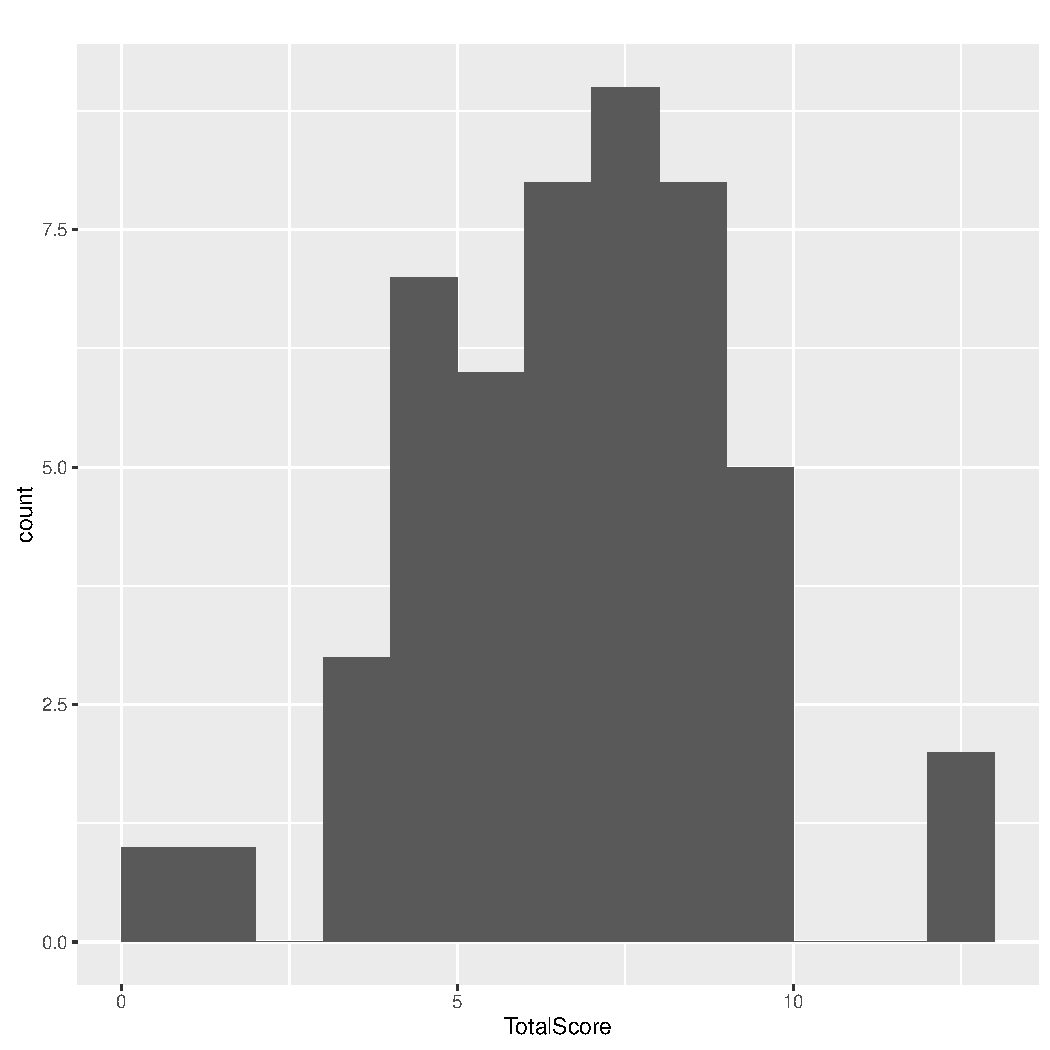
\includegraphics[width=0.98\linewidth]{/Users/lindz/ePort/inst/extdata/OutputFiles/histScore-1} \caption[Histogram of scores]{Histogram of scores.}\label{mar:histScore}
\end{marginfigure}


\end{knitrout}

% latex table generated in R 3.2.2 by xtable 1.8-0 package
% Thu Jan 21 00:33:10 2016
\begin{longtable}{rrlrrrrr}
  \hline
Mean & Std.dev &   & Min & Q1 & Median & Q3 & Max \\ 
  \hline
6.24 & 2.38 &  & 0.00 & 5.00 & 6.00 & 8.00 & 12.00 \\ 
   \hline
\hline
\caption{Summary statistics of the scores} 
\label{tab:summary}
\end{longtable}


\clearpage
\newpage{}
\section{Topic Learning Outcomes}

\bigskip{}

\begin{fullwidth}
\begin{enumerate}[label=\Alph*.,itemsep=-\parsep,leftmargin=*]
  \item
Use standardizing to determine how many standard deviations an observation is away from the mean value.
\item Use z-scores to compare observations for different quantitative variables.
\item Explain how standardizing affects the shape, center, and variability of the distribution of a quantitative variable.
\item Determine which quantitative variables could be modeled using the normal distribution by interpreting graphical representations of the variable.
\item Apply the 68-95-99.
\item Find percentile or area values for any given observation from a normal distribution.
\item Find the value of an observation when given a percentile or area value from the normal distribution.

\end{enumerate}
\end{fullwidth}

\newpage{}

Table \ref{tab:LearningObj_summary} and Figure \ref{mar:LearningObjSummary} show the summary of percentage scores by learning outcome.
Among all learning outcomes, Outcome
D
has the highest correct percentage, while Outcome
E
has the lowest.



\begin{knitrout}
\definecolor{shadecolor}{rgb}{0.969, 0.969, 0.969}\color{fgcolor}\begin{marginfigure}
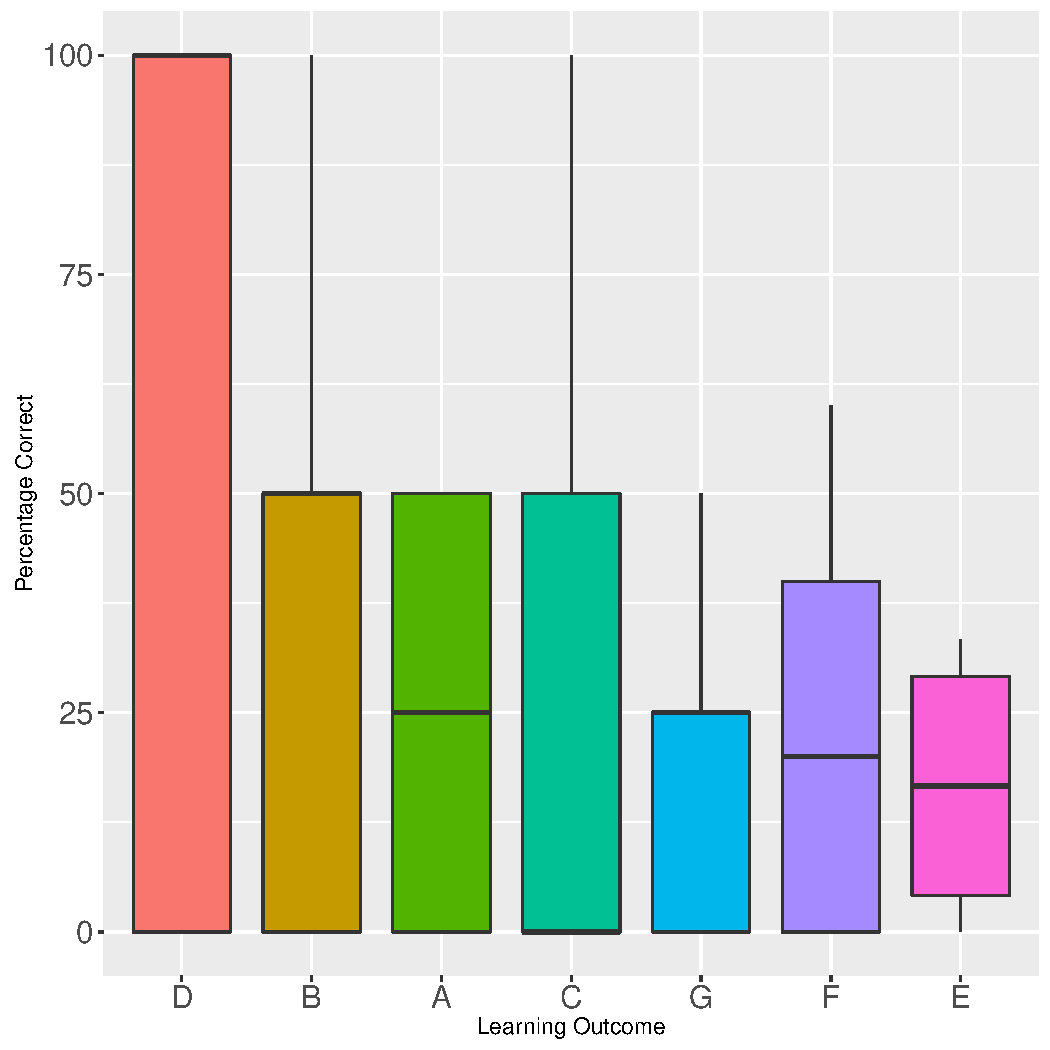
\includegraphics[width=0.98\linewidth]{/Users/lindz/ePort/inst/extdata/OutputFiles/LearningObjSummary-1} \caption[Side-by-side boxplots of the correct percentages by learning outcome]{Side-by-side boxplots of the correct percentages by learning outcome.}\label{mar:LearningObjSummary}
\end{marginfigure}


\end{knitrout}

% latex table generated in R 3.2.2 by xtable 1.8-0 package
% Thu Jan 21 00:33:11 2016
\begin{longtable}{rrrllrrr}
  \hline
 & Mean & Std.dev &   &   & Min & Median & Max \\ 
  \hline
D & 61.00 & 45.50 &  &  & 0.00 & 100.00 & 100.00 \\ 
  B & 38.00 & 37.20 &  &  & 0.00 & 50.00 & 100.00 \\ 
  A & 23.00 & 20.73 &  &  & 0.00 & 25.00 & 50.00 \\ 
  C & 22.00 & 27.03 &  &  & 0.00 & 0.00 & 100.00 \\ 
  G & 21.50 & 18.22 &  &  & 0.00 & 25.00 & 50.00 \\ 
  F & 20.80 & 19.78 &  &  & 0.00 & 20.00 & 60.00 \\ 
  E & 16.67 & 12.14 &  &  & 0.00 & 16.67 & 33.33 \\ 
   \hline
\hline
\caption{Summary statistics of the student percentage correct scores on the topic learning outcomes. The table is sorted from the highest mean to the lowest.} 
\label{tab:LearningObj_summary}
\end{longtable}






To analyze the students' performance on different learning outcomes, we consider the generalized mixed effects model:
\[
g(E[Y_{ij}|u_{j}])= \tau_{i}+u_{j}
\]
where $i=1,...,$7 learning outcomes;
$j=1,...,$50 students. $Y_{ij}$ is the score (scaled in $[0,1]$) of
the $j$th student in the $i$th learning outcome. $\tau_i$ is the fixed effect,
which represents the actual level of the learning outcome $i$.
$u_j$ is the random effect from the students with
$u_{j} \sim N(0,\sigma_{u}^{2})$.

Since $Y_{ij} \in [0,1]$, and most of $y_{ij}$ take the value 1
(see Figure \ref{mar:crtpctHist}), it is not easy to find an appropriate model.
Beta distribution is possible if 0 and 1 are not in the range of $Y_{ij}$.
Binomial distribution is another possibility if we do not scale the scores.
Hence we assume that $Y$ is binomial with the logit link function,
then the results are in Table \ref{tab:lme_fixed} and Figure \ref{mar:lmeCoef}.

\begin{knitrout}
\definecolor{shadecolor}{rgb}{0.969, 0.969, 0.969}\color{fgcolor}\begin{marginfigure}
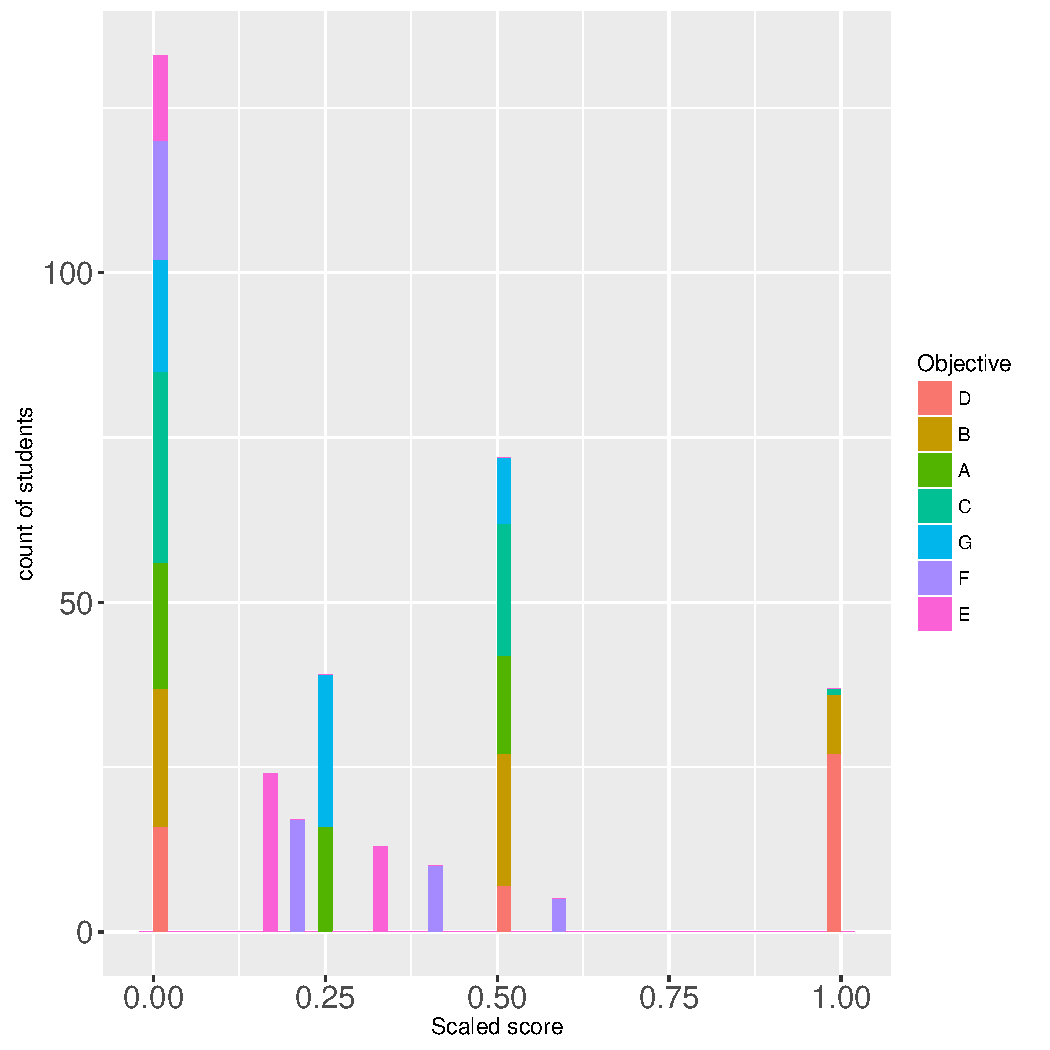
\includegraphics[width=0.99\linewidth]{/Users/lindz/ePort/inst/extdata/OutputFiles/crtpctHist-1} \caption[Histogram of the scaled scores by learning outcome]{Histogram of the scaled scores by learning outcome.}\label{mar:crtpctHist}
\end{marginfigure}


\end{knitrout}

% latex table generated in R 3.2.2 by xtable 1.8-0 package
% Thu Jan 21 00:33:12 2016
\begin{longtable}{rrlrr}
  \hline
 & est. &    & lower & upper \\ 
  \hline
(Intercept) & 0.44 &  & 0.10 & 0.79 \\ 
  ObjectiveB & -0.93 &  & -1.40 & -0.47 \\ 
  ObjectiveA & -1.64 &  & -2.14 & -1.14 \\ 
  ObjectiveC & -1.70 &  & -2.20 & -1.19 \\ 
  ObjectiveG & -1.72 &  & -2.23 & -1.22 \\ 
  ObjectiveF & -1.76 &  & -2.28 & -1.25 \\ 
  ObjectiveE & -2.03 &  & -2.56 & -1.49 \\ 
   \hline
\hline
\caption{95\% confidence intervals of the fixed effects} 
\label{tab:lme_fixed}
\end{longtable}


It shows that D is the best understood learning outcome.
Outcomes E,F,G,C,A,B are
significantly worse than D.



\begin{knitrout}
\definecolor{shadecolor}{rgb}{0.969, 0.969, 0.969}\color{fgcolor}\begin{marginfigure}
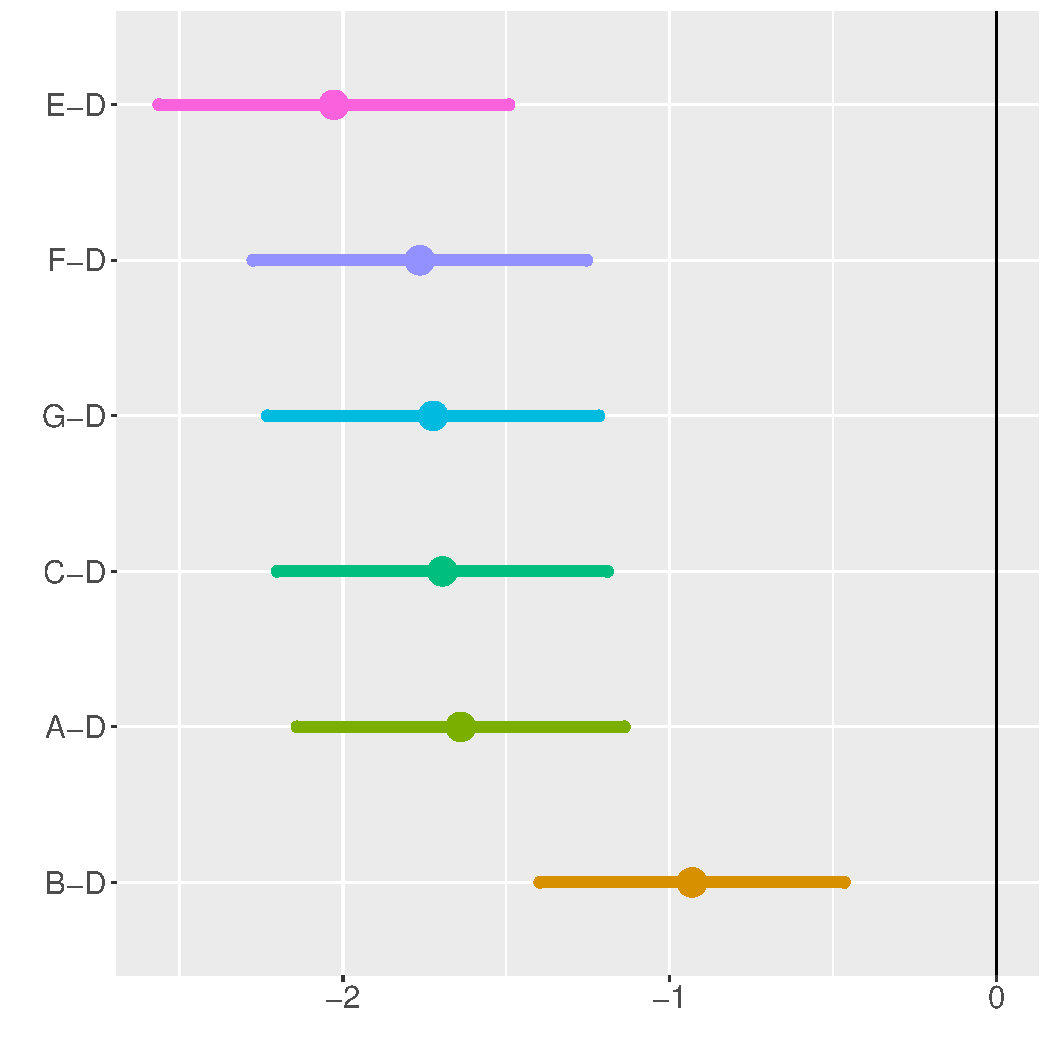
\includegraphics[width=0.99\linewidth]{/Users/lindz/ePort/inst/extdata/OutputFiles/lmeCoef-1} \caption[95\% confidence intervals of the fixed effects coefficients]{95\% confidence intervals of the fixed effects coefficients}\label{mar:lmeCoef}
\end{marginfigure}


\end{knitrout}

Nevertheless, the assumption is probably incorrect, as we could check the residuals in
Figure \ref{fig:lmeQQNorm}.

\begin{knitrout}
\definecolor{shadecolor}{rgb}{0.969, 0.969, 0.969}\color{fgcolor}\begin{figure}

{\centering 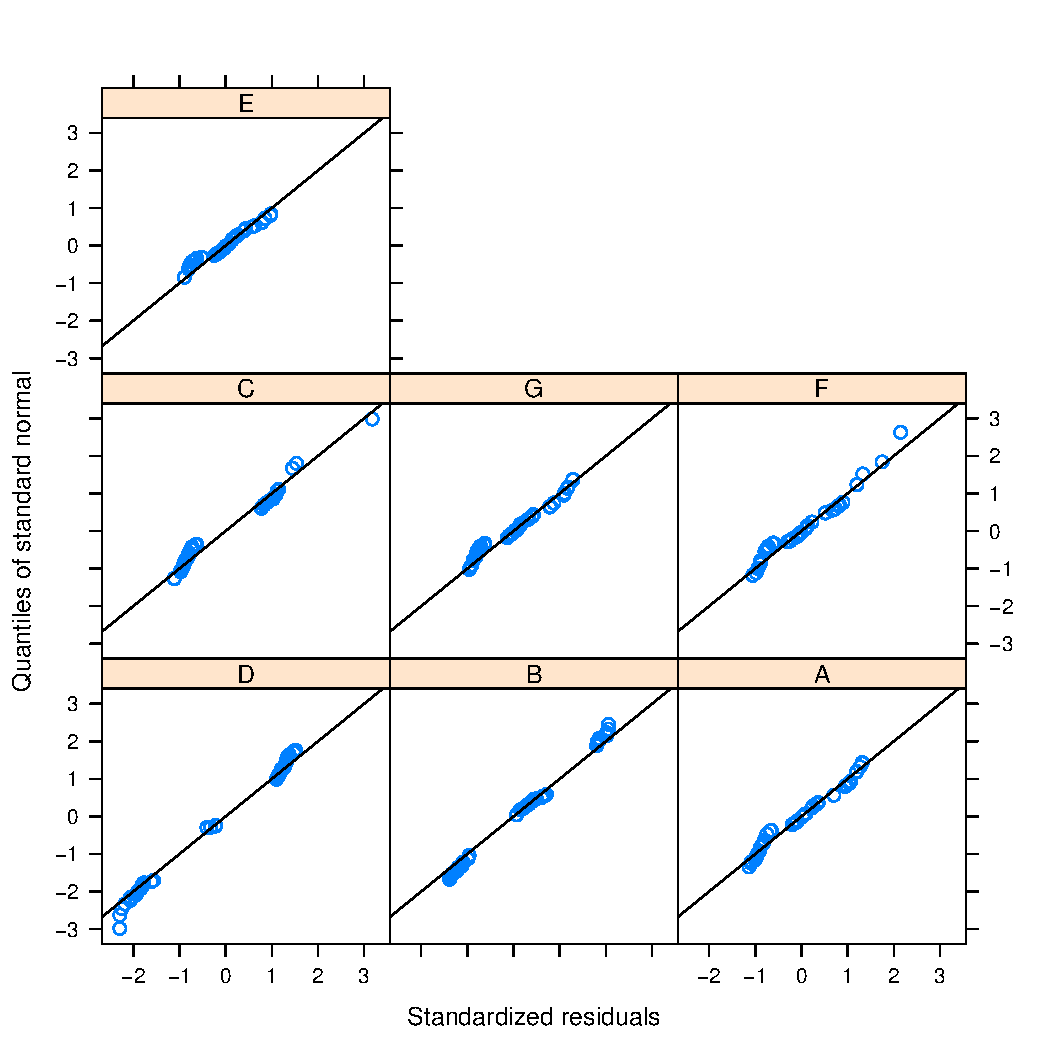
\includegraphics[width=0.98\linewidth]{/Users/lindz/ePort/inst/extdata/OutputFiles/lmeQQNorm-1} 

}

\caption[QQ-plot of the residuals by the generalized mixed effects model]{QQ-plot of the residuals by the generalized mixed effects model}\label{fig:lmeQQNorm}
\end{figure}


\end{knitrout}

\clearpage
\newpage{}
\subsection{Question Sets}

Table \ref{tab:QuestionSet_summary} and Figure \ref{mar:questionSetBoxplot} shows the summary statistics of the percentage correct score by question for each question set. Percentage correct scores for questions in the same question set should have small variability.
%As is shown, Question Set colnames(sumry2$SetCorrectPct)[which.max(sumry2$SetCorrectPct[1,])] has the highest mean correct percentage and question set colnames(sumry2$SetCorrectPct)[which.min(sumry2$SetCorrectPct[1,])] has the lowest mean.


% latex table generated in R 3.2.2 by xtable 1.8-0 package
% Thu Jan 21 00:33:14 2016
\begin{longtable}{cc|ccc|ccc}
  \hline
Qset & LO & \# & Mean & Std.dev & Min & Median & Max \\ 
  \hline
S & G &   5 & 23.39 & 19.03 & 0.00 & 27.27 & 50.00 \\ 
  Q & F &   5 & 28.71 & 18.83 & 0.00 & 28.57 & 50.00 \\ 
  B & A &   4 & 46.13 & 17.26 & 25.00 & 46.43 & 66.67 \\ 
  J & D &   4 & 62.08 & 14.74 & 50.00 & 57.50 & 83.33 \\ 
  N & F &   5 & 18.95 & 14.61 & 0.00 & 20.00 & 37.50 \\ 
  L & E &   9 & 23.02 & 14.35 & 5.56 & 26.32 & 42.11 \\ 
  U & G &   5 & 20.00 & 13.94 & 0.00 & 16.67 & 33.33 \\ 
  R & G &   5 & 16.71 & 13.21 & 0.00 & 20.00 & 33.33 \\ 
  M & F &   5 & 31.24 & 12.06 & 25.00 & 25.00 & 52.63 \\ 
  O & F &   5 & 11.65 & 12.03 & 0.00 & 14.29 & 28.57 \\ 
  T & G &   5 & 14.98 & 11.41 & 0.00 & 14.29 & 27.27 \\ 
  K & E &   9 & 9.56 & 10.68 & 0.00 & 5.88 & 31.25 \\ 
  A & A &   4 & 42.27 & 9.74 & 30.00 & 43.08 & 52.94 \\ 
  P & F &   5 & 6.51 & 6.46 & 0.00 & 7.14 & 14.29 \\ 
  I & D &   2 & 64.16 & 1.18 & 63.33 & 64.16 & 65.00 \\ 
  C & A &   4 & 0.00 & 0.00 & 0.00 & 0.00 & 0.00 \\ 
  D & A &   4 & 0.00 & 0.00 & 0.00 & 0.00 & 0.00 \\ 
  E & B &   1 & 40.00 & 0.00 & 40.00 & 40.00 & 40.00 \\ 
  F & B &   1 & 36.00 & 0.00 & 36.00 & 36.00 & 36.00 \\ 
  G & C &   1 & 20.00 & 0.00 & 20.00 & 20.00 & 20.00 \\ 
  H & C &   1 & 24.00 & 0.00 & 24.00 & 24.00 & 24.00 \\ 
   \hline
\hline
\caption{Summary statistics of the percentage correct score by question for each question sets. The table is sorted from the largest standard deviation to the smallest.} 
\label{tab:QuestionSet_summary}
\end{longtable}


\begin{knitrout}
\definecolor{shadecolor}{rgb}{0.969, 0.969, 0.969}\color{fgcolor}\begin{marginfigure}

{\centering 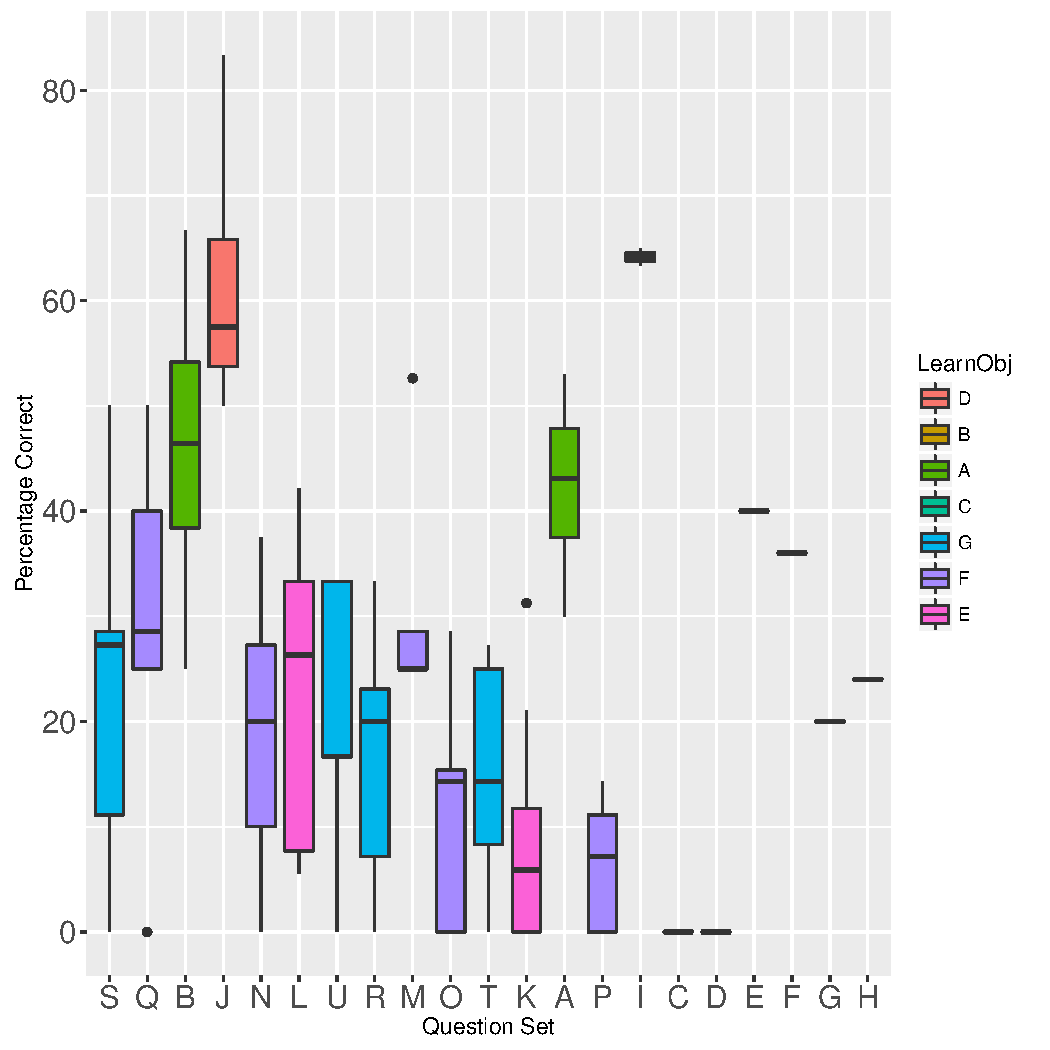
\includegraphics[width=0.99\linewidth]{/Users/lindz/ePort/inst/extdata/OutputFiles/questionSetBoxplot-1} 

}

\caption[Side-by-side boxplots of the question correct percentage score for each question set]{Side-by-side boxplots of the question correct percentage score for each question set}\label{fig:questionSetBoxplot}
\end{marginfigure}


\end{knitrout}

\clearpage
\newpage{}
\subsection{Questions}

Table \ref{tab:summary_question} compares the performance on each question.



% latex table generated in R 3.2.2 by xtable 1.8-0 package
% Thu Jan 21 00:33:16 2016
\begin{longtable}{cccl|cccc|ccccc|l}
  \hline
ID & LO & Qset & Name & Type & FullPt & QinSet & N & CrtPct & Count & NA's & Mean & Std & Flag \\ 
  \hline
\hyperlink{T06.A.A.04.1.1.MC.1.2}{1} & A & A & 1 & MC &   1 &   1 &   4 & 40.00 &  10 &  40 & 0.40 & 0.52 &  \\ 
  \hyperlink{T06.A.A.04.1.1.MC.2.2}{2} & A & A & 2 & MC &   1 &   1 &   4 & 46.15 &  13 &  37 & 0.46 & 0.52 & * \\ 
  \hyperlink{T06.A.A.04.1.1.MC.3.2}{3} & A & A & 3 & MC &   1 &   1 &   4 & 30.00 &  10 &  40 & 0.30 & 0.48 & * \\ 
  \hyperlink{T06.A.A.04.1.1.MC.4.2}{4} & A & A & 4 & MC &   1 &   1 &   4 & 52.94 &  17 &  33 & 0.53 & 0.51 & * \\ 
   &  &  &  &  &  &  &  &  &  &  &  &  &  \\ 
  \hyperlink{T06.A.B.04.1.1.MC.1.2}{5} & A & B & 1 & MC &   1 &   1 &   4 & 42.86 &  14 &  36 & 0.43 & 0.51 & * \\ 
  \hyperlink{T06.A.B.04.1.1.MC.2.2}{6} & A & B & 2 & MC &   1 &   1 &   4 & 50.00 &  16 &  34 & 0.50 & 0.52 & * \\ 
  \hyperlink{T06.A.B.04.1.1.MC.3.2}{7} & A & B & 3 & MC &   1 &   1 &   4 & 25.00 &   8 &  42 & 0.25 & 0.46 & * \\ 
  \hyperlink{T06.A.B.04.1.1.MC.4.2}{8} & A & B & 4 & MC &   1 &   1 &   4 & 66.67 &  12 &  38 & 0.67 & 0.49 & * \\ 
   &  &  &  &  &  &  &  &  &  &  &  &  &  \\ 
  \hyperlink{T06.A.C.04.1.1.FB.1.2}{9} & A & C & 1 & FB &   1 &   1 &   4 & 0.00 &  11 &  39 & 0.00 & 0.00 &  \\ 
  \hyperlink{T06.A.C.04.1.1.FB.2.2}{10} & A & C & 2 & FB &   1 &   1 &   4 & 0.00 &  11 &  39 & 0.00 & 0.00 &  \\ 
  \hyperlink{T06.A.C.04.1.1.FB.3.2}{11} & A & C & 3 & FB &   1 &   1 &   4 & 0.00 &  14 &  36 & 0.00 & 0.00 &  \\ 
  \hyperlink{T06.A.C.04.1.1.FB.4.2}{12} & A & C & 4 & FB &   1 &   1 &   4 & 0.00 &  14 &  36 & 0.00 & 0.00 &  \\ 
   &  &  &  &  &  &  &  &  &  &  &  &  &  \\ 
  \hyperlink{T06.A.D.04.1.1.FB.1.2}{13} & A & D & 1 & FB &   1 &   1 &   4 & 0.00 &  10 &  40 & 0.00 & 0.00 &  \\ 
  \hyperlink{T06.A.D.04.1.1.FB.2.2}{14} & A & D & 2 & FB &   1 &   1 &   4 & 0.00 &  13 &  37 & 0.00 & 0.00 &  \\ 
  \hyperlink{T06.A.D.04.1.1.FB.3.2}{15} & A & D & 3 & FB &   1 &   1 &   4 & 0.00 &  11 &  39 & 0.00 & 0.00 &  \\ 
  \hyperlink{T06.A.D.04.1.1.FB.4.2}{16} & A & D & 4 & FB &   1 &   1 &   4 & 0.00 &  16 &  34 & 0.00 & 0.00 &  \\ 
   &  &  &  &  &  &  &  &  &  &  &  &  &  \\ 
  \hyperlink{T06.B.E.01.1.1.MC.compare1.2}{17} & B & E & compare1 & MC &   1 &   1 &   1 & 40.00 &  50 &   0 & 0.40 & 0.49 &  \\ 
   &  &  &  &  &  &  &  &  &  &  &  &  &  \\ 
  \hyperlink{T06.B.F.01.1.1.MC.compare2.2}{18} & B & F & compare2 & MC &   1 &   1 &   1 & 36.00 &  50 &   0 & 0.36 & 0.48 &  \\ 
   &  &  &  &  &  &  &  &  &  &  &  &  &  \\ 
  \hyperlink{T06.C.G.01.1.1.MC.1.2}{19} & C & G & 1 & MC &   1 &   1 &   1 & 20.00 &  50 &   0 & 0.20 & 0.40 &  \\ 
   &  &  &  &  &  &  &  &  &  &  &  &  &  \\ 
  \hyperlink{T06.C.H.01.1.1.MC.1.2}{20} & C & H & 1 & MC &   1 &   1 &   1 & 24.00 &  50 &   0 & 0.24 & 0.43 &  \\ 
   &  &  &  &  &  &  &  &  &  &  &  &  &  \\ 
  \hyperlink{T06.D.I.02.1.1.TF.feet.2}{21} & D & I & feet & TF &   1 &   1 &   2 & 65.00 &  20 &  30 & 0.65 & 0.49 &  \\ 
  \hyperlink{T06.D.I.02.1.1.TF.lowtemp.2}{22} & D & I & lowtemp & TF &   1 &   1 &   2 & 63.33 &  30 &  20 & 0.63 & 0.49 &  \\ 
   &  &  &  &  &  &  &  &  &  &  &  &  &  \\ 
  \hyperlink{T06.D.J.04.1.1.TF.gain.2}{23} & D & J & gain & TF &   1 &   1 &   4 & 60.00 &  10 &  40 & 0.60 & 0.52 & * \\ 
  \hyperlink{T06.D.J.04.1.1.TF.mpg.2}{24} & D & J & mpg & TF &   1 &   1 &   4 & 83.33 &   6 &  44 & 0.83 & 0.41 & * \\ 
  \hyperlink{T06.D.J.04.1.1.TF.blowhole.2}{25} & D & J & blowhole & TF &   1 &   1 &   4 & 50.00 &  14 &  36 & 0.50 & 0.52 & * \\ 
  \hyperlink{T06.D.J.04.1.1.TF.CDs.2}{26} & D & J & CDs & TF &   1 &   1 &   4 & 55.00 &  20 &  30 & 0.55 & 0.51 & * \\ 
   &  &  &  &  &  &  &  &  &  &  &  &  &  \\ 
  \hyperlink{T06.E.K.09.3.1.FB.whale1.2}{27} & E & K & whale1 & FB &   1 &   3 &   9 & 21.05 &  19 &  31 & 0.21 & 0.42 & * \\ 
  \hyperlink{T06.E.K.09.3.1.FB.whale2.2}{28} & E & K & whale2 & FB &   1 &   3 &   9 & 0.00 &  18 &  32 & 0.00 & 0.00 & * \\ 
  \hyperlink{T06.E.K.09.3.1.FB.whale3.2}{29} & E & K & whale3 & FB &   1 &   3 &   9 & 0.00 &  14 &  36 & 0.00 & 0.00 & * \\ 
  \hyperlink{T06.E.K.09.3.1.FB.cow1.2}{30} & E & K & cow1 & FB &   1 &   3 &   9 & 0.00 &  12 &  38 & 0.00 & 0.00 & * \\ 
  \hyperlink{T06.E.K.09.3.1.FB.cow2.2}{31} & E & K & cow2 & FB &   1 &   3 &   9 & 5.56 &  18 &  32 & 0.06 & 0.24 & * \\ 
  \hyperlink{T06.E.K.09.3.1.FB.cow3.2}{32} & E & K & cow3 & FB &   1 &   3 &   9 & 11.76 &  17 &  33 & 0.12 & 0.33 & * \\ 
  \hyperlink{T06.E.K.09.3.1.FB.bulbs1.2}{33} & E & K & bulbs1 & FB &   1 &   3 &   9 & 31.25 &  16 &  34 & 0.31 & 0.48 & * \\ 
  \hyperlink{T06.E.K.09.3.1.FB.bulbs2.2}{34} & E & K & bulbs2 & FB &   1 &   3 &   9 & 5.88 &  17 &  33 & 0.06 & 0.24 & * \\ 
  \hyperlink{T06.E.K.09.3.1.FB.bulbs3.2}{35} & E & K & bulbs3 & FB &   1 &   3 &   9 & 10.53 &  19 &  31 & 0.11 & 0.32 & * \\ 
   &  &  &  &  &  &  &  &  &  &  &  &  &  \\ 
  \hyperlink{T06.E.L.09.3.1.MC.heights1.2}{36} & E & L & heights1 & MC &   1 &   3 &   9 & 15.79 &  19 &  31 & 0.16 & 0.37 & * \\ 
  \hyperlink{T06.E.L.09.3.1.MC.heights2.2}{37} & E & L & heights2 & MC &   1 &   3 &   9 & 5.56 &  18 &  32 & 0.06 & 0.24 & * \\ 
  \hyperlink{T06.E.L.09.3.1.MC.heights3.2}{38} & E & L & heights3 & MC &   1 &   3 &   9 & 42.11 &  19 &  31 & 0.42 & 0.51 & * \\ 
  \hyperlink{T06.E.L.09.3.1.MC.mm1.2}{39} & E & L & mm1 & MC &   1 &   3 &   9 & 7.69 &  13 &  37 & 0.08 & 0.28 & * \\ 
  \hyperlink{T06.E.L.09.3.1.MC.mm2.2}{40} & E & L & mm2 & MC &   1 &   3 &   9 & 31.25 &  16 &  34 & 0.31 & 0.48 & * \\ 
  \hyperlink{T06.E.L.09.3.1.MC.mm3.2}{41} & E & L & mm3 & MC &   1 &   3 &   9 & 26.32 &  19 &  31 & 0.26 & 0.45 & * \\ 
  \hyperlink{T06.E.L.09.3.1.MC.IQ1.2}{42} & E & L & IQ1 & MC &   1 &   3 &   9 & 33.33 &  18 &  32 & 0.33 & 0.49 & * \\ 
  \hyperlink{T06.E.L.09.3.1.MC.IQ2.2}{43} & E & L & IQ2 & MC &   1 &   3 &   9 & 38.46 &  13 &  37 & 0.38 & 0.51 & * \\ 
  \hyperlink{T06.E.L.09.3.1.MC.IQ3.2}{44} & E & L & IQ3 & MC &   1 &   3 &   9 & 6.67 &  15 &  35 & 0.07 & 0.26 & * \\ 
   &  &  &  &  &  &  &  &  &  &  &  &  &  \\ 
  \hyperlink{T06.F.M.05.1.1.MC.mm1.2}{45} & F & M & mm1 & MC &   1 &   1 &   5 & 52.63 &  19 &  31 & 0.53 & 0.51 & * \\ 
  \hyperlink{T06.F.M.05.1.1.MC.Bulb1.2}{46} & F & M & Bulb1 & MC &   1 &   1 &   5 & 25.00 &   8 &  42 & 0.25 & 0.46 & * \\ 
  \hyperlink{T06.F.M.05.1.1.MC.IQ1.2}{47} & F & M & IQ1 & MC &   1 &   1 &   5 & 25.00 &   8 &  42 & 0.25 & 0.46 & * \\ 
  \hyperlink{T06.F.M.05.1.1.MC.Whale1.2}{48} & F & M & Whale1 & MC &   1 &   1 &   5 & 28.57 &   7 &  43 & 0.29 & 0.49 & * \\ 
  \hyperlink{T06.F.M.05.1.1.MC.Cow1.2}{49} & F & M & Cow1 & MC &   1 &   1 &   5 & 25.00 &   8 &  42 & 0.25 & 0.46 & * \\ 
   &  &  &  &  &  &  &  &  &  &  &  &  &  \\ 
  \hyperlink{T06.F.N.05.1.1.MC.mm2.2}{50} & F & N & mm2 & MC &   1 &   1 &   5 & 37.50 &   8 &  42 & 0.38 & 0.52 & * \\ 
  \hyperlink{T06.F.N.05.1.1.MC.Bulb2.2}{51} & F & N & Bulb2 & MC &   1 &   1 &   5 & 0.00 &  11 &  39 & 0.00 & 0.00 & * \\ 
  \hyperlink{T06.F.N.05.1.1.MC.IQ2.2}{52} & F & N & IQ2 & MC &   1 &   1 &   5 & 27.27 &  11 &  39 & 0.27 & 0.47 & * \\ 
  \hyperlink{T06.F.N.05.1.1.MC.Whale2.2}{53} & F & N & Whale2 & MC &   1 &   1 &   5 & 10.00 &  10 &  40 & 0.10 & 0.32 & * \\ 
  \hyperlink{T06.F.N.05.1.1.MC.Cow2.2}{54} & F & N & Cow2 & MC &   1 &   1 &   5 & 20.00 &  10 &  40 & 0.20 & 0.42 & * \\ 
   &  &  &  &  &  &  &  &  &  &  &  &  &  \\ 
  \hyperlink{T06.F.O.05.1.1.MC.mm3.2}{55} & F & O & mm3 & MC &   1 &   1 &   5 & 14.29 &   7 &  43 & 0.14 & 0.38 &  \\ 
  \hyperlink{T06.F.O.05.1.1.MC.Bulb3.2}{56} & F & O & Bulb3 & MC &   1 &   1 &   5 & 0.00 &   8 &  42 & 0.00 & 0.00 & * \\ 
  \hyperlink{T06.F.O.05.1.1.MC.IQ3.2}{57} & F & O & IQ3 & MC &   1 &   1 &   5 & 0.00 &   8 &  42 & 0.00 & 0.00 & * \\ 
  \hyperlink{T06.F.O.05.1.1.MC.Whale3.2}{58} & F & O & Whale3 & MC &   1 &   1 &   5 & 28.57 &  14 &  36 & 0.29 & 0.47 & * \\ 
  \hyperlink{T06.F.O.05.1.1.MC.Cow3.2}{59} & F & O & Cow3 & MC &   1 &   1 &   5 & 15.38 &  13 &  37 & 0.15 & 0.38 & * \\ 
   &  &  &  &  &  &  &  &  &  &  &  &  &  \\ 
  \hyperlink{T06.F.P.05.1.1.MC.mm4.2}{60} & F & P & mm4 & MC &   1 &   1 &   5 & 7.14 &  14 &  36 & 0.07 & 0.27 &  \\ 
  \hyperlink{T06.F.P.05.1.1.MC.Bulb4.2}{61} & F & P & Bulb4 & MC &   1 &   1 &   5 & 0.00 &   7 &  43 & 0.00 & 0.00 &  \\ 
  \hyperlink{T06.F.P.05.1.1.MC.IQ4.2}{62} & F & P & IQ4 & MC &   1 &   1 &   5 & 14.29 &   7 &  43 & 0.14 & 0.38 &  \\ 
  \hyperlink{T06.F.P.05.1.1.MC.Whale4.2}{63} & F & P & Whale4 & MC &   1 &   1 &   5 & 0.00 &  13 &  37 & 0.00 & 0.00 &  \\ 
  \hyperlink{T06.F.P.05.1.1.MC.Cow4.2}{64} & F & P & Cow4 & MC &   1 &   1 &   5 & 11.11 &   9 &  41 & 0.11 & 0.33 &  \\ 
   &  &  &  &  &  &  &  &  &  &  &  &  &  \\ 
  \hyperlink{T06.F.Q.05.1.1.MC.mm5.2}{65} & F & Q & mm5 & MC &   1 &   1 &   5 & 50.00 &   4 &  46 & 0.50 & 0.58 & * \\ 
  \hyperlink{T06.F.Q.05.1.1.MC.Bulb5.2}{66} & F & Q & Bulb5 & MC &   1 &   1 &   5 & 25.00 &  12 &  38 & 0.25 & 0.45 & * \\ 
  \hyperlink{T06.F.Q.05.1.1.MC.IQ5.2}{67} & F & Q & IQ5 & MC &   1 &   1 &   5 & 0.00 &   7 &  43 & 0.00 & 0.00 & * \\ 
  \hyperlink{T06.F.Q.05.1.1.MC.Whale5.2}{68} & F & Q & Whale5 & MC &   1 &   1 &   5 & 28.57 &   7 &  43 & 0.29 & 0.49 & * \\ 
  \hyperlink{T06.F.Q.05.1.1.MC.Cow5.2}{69} & F & Q & Cow5 & MC &   1 &   1 &   5 & 40.00 &  20 &  30 & 0.40 & 0.50 & * \\ 
   &  &  &  &  &  &  &  &  &  &  &  &  &  \\ 
  \hyperlink{T06.G.R.05.1.1.MC.mm1.2}{70} & G & R & mm1 & MC &   1 &   1 &   5 & 20.00 &  10 &  40 & 0.20 & 0.42 & * \\ 
  \hyperlink{T06.G.R.05.1.1.MC.Bulb1.2}{71} & G & R & Bulb1 & MC &   1 &   1 &   5 & 7.14 &  14 &  36 & 0.07 & 0.27 & * \\ 
  \hyperlink{T06.G.R.05.1.1.MC.IQ1.2}{72} & G & R & IQ1 & MC &   1 &   1 &   5 & 0.00 &   4 &  46 & 0.00 & 0.00 & * \\ 
  \hyperlink{T06.G.R.05.1.1.MC.Whale1.2}{73} & G & R & Whale1 & MC &   1 &   1 &   5 & 23.08 &  13 &  37 & 0.23 & 0.44 & * \\ 
  \hyperlink{T06.G.R.05.1.1.MC.Cow1.2}{74} & G & R & Cow1 & MC &   1 &   1 &   5 & 33.33 &   9 &  41 & 0.33 & 0.50 & * \\ 
   &  &  &  &  &  &  &  &  &  &  &  &  &  \\ 
  \hyperlink{T06.G.S.05.1.1.MC.mm2.2}{75} & G & S & mm2 & MC &   1 &   1 &   5 & 50.00 &  14 &  36 & 0.50 & 0.52 & * \\ 
  \hyperlink{T06.G.S.05.1.1.MC.Bulb2.2}{76} & G & S & Bulb2 & MC &   1 &   1 &   5 & 27.27 &  11 &  39 & 0.27 & 0.47 & * \\ 
  \hyperlink{T06.G.S.05.1.1.MC.IQ2.2}{77} & G & S & IQ2 & MC &   1 &   1 &   5 & 0.00 &   9 &  41 & 0.00 & 0.00 & * \\ 
  \hyperlink{T06.G.S.05.1.1.MC.Whale2.2}{78} & G & S & Whale2 & MC &   1 &   1 &   5 & 11.11 &   9 &  41 & 0.11 & 0.33 & * \\ 
  \hyperlink{T06.G.S.05.1.1.MC.Cow2.2}{79} & G & S & Cow2 & MC &   1 &   1 &   5 & 28.57 &   7 &  43 & 0.29 & 0.49 & * \\ 
   &  &  &  &  &  &  &  &  &  &  &  &  &  \\ 
  \hyperlink{T06.G.T.05.1.1.MC.mm3.2}{80} & G & T & mm3 & MC &   1 &   1 &   5 & 27.27 &  11 &  39 & 0.27 & 0.47 & * \\ 
  \hyperlink{T06.G.T.05.1.1.MC.Bulb3.2}{81} & G & T & Bulb3 & MC &   1 &   1 &   5 & 25.00 &   8 &  42 & 0.25 & 0.46 & * \\ 
  \hyperlink{T06.G.T.05.1.1.MC.IQ3.2}{82} & G & T & IQ3 & MC &   1 &   1 &   5 & 14.29 &  14 &  36 & 0.14 & 0.36 &  \\ 
  \hyperlink{T06.G.T.05.1.1.MC.Whale3.2}{83} & G & T & Whale3 & MC &   1 &   1 &   5 & 0.00 &   5 &  45 & 0.00 & 0.00 & * \\ 
  \hyperlink{T06.G.T.05.1.1.MC.Cow3.2}{84} & G & T & Cow3 & MC &   1 &   1 &   5 & 8.33 &  12 &  38 & 0.08 & 0.29 & * \\ 
   &  &  &  &  &  &  &  &  &  &  &  &  &  \\ 
  \hyperlink{T06.G.U.05.1.1.MC.mm4.2}{85} & G & U & mm4 & MC &   1 &   1 &   5 & 0.00 &   5 &  45 & 0.00 & 0.00 & * \\ 
  \hyperlink{T06.G.U.05.1.1.MC.Bulb4.2}{86} & G & U & Bulb4 & MC &   1 &   1 &   5 & 33.33 &  12 &  38 & 0.33 & 0.49 & * \\ 
  \hyperlink{T06.G.U.05.1.1.MC.IQ4.2}{87} & G & U & IQ4 & MC &   1 &   1 &   5 & 33.33 &  21 &  29 & 0.33 & 0.48 & * \\ 
  \hyperlink{T06.G.U.05.1.1.MC.Whale4.2}{88} & G & U & Whale4 & MC &   1 &   1 &   5 & 16.67 &   6 &  44 & 0.17 & 0.41 & * \\ 
  \hyperlink{T06.G.U.05.1.1.MC.Cow4.2}{89} & G & U & Cow4 & MC &   1 &   1 &   5 & 16.67 &   6 &  44 & 0.17 & 0.41 & * \\ 
   \hline
\hline
\caption{Summary statistics of each question} 
\label{tab:summary_question}
\end{longtable}


\clearpage
\newpage{}
\section{Students}
The percentages correct by learning outcome and total for each student, sorted by the highest to lowest total are displayed in Table \ref{tab:LearningObj_data}. And the ranks in percentage are given in Table \ref{tab:LearningObj_rank}. Figure \ref{fig:LearningObj_rank} shows the percent rank of the students.

% latex table generated in R 3.2.2 by xtable 1.8-0 package
% Thu Jan 21 00:33:16 2016
\begin{longtable}{rrrrrrrrr}
  \hline
 & Total & E & F & G & C & A & B & D \\ 
  \hline
 &  &  &  &  &  &  &  &  \\ 
  w.introstat40 & 48.00 & 33.33 & 60.00 & 50.00 & 0.00 & 50.00 & 50.00 & 100.00 \\ 
  w.introStat50 & 48.00 & 33.33 & 60.00 & 50.00 & 0.00 & 50.00 & 50.00 & 100.00 \\ 
  w.introstat26 & 36.00 & 16.67 & 60.00 & 25.00 & 50.00 & 0.00 & 50.00 & 100.00 \\ 
  w.introstat39 & 36.00 & 16.67 & 20.00 & 50.00 & 50.00 & 0.00 & 100.00 & 100.00 \\ 
  w.introstat42 & 36.00 & 33.33 & 0.00 & 25.00 & 50.00 & 25.00 & 100.00 & 100.00 \\ 
  w.introStat52 & 36.00 & 33.33 & 0.00 & 25.00 & 50.00 & 25.00 & 100.00 & 100.00 \\ 
  w.introstat65 & 36.00 & 16.67 & 20.00 & 50.00 & 50.00 & 25.00 & 50.00 & 100.00 \\ 
  w.introstat33 & 32.00 & 16.67 & 40.00 & 50.00 & 50.00 & 25.00 & 50.00 & 0.00 \\ 
  w.introstat34 & 32.00 & 33.33 & 0.00 & 25.00 & 50.00 & 25.00 & 50.00 & 100.00 \\ 
  w.introstat37 & 32.00 & 16.67 & 40.00 & 0.00 & 0.00 & 50.00 & 50.00 & 100.00 \\ 
  w.introstat45 & 32.00 & 33.33 & 40.00 & 50.00 & 0.00 & 50.00 & 0.00 & 0.00 \\ 
  w.introstat49 & 32.00 & 0.00 & 40.00 & 25.00 & 50.00 & 0.00 & 100.00 & 100.00 \\ 
  w.introStat55 & 32.00 & 33.33 & 40.00 & 50.00 & 0.00 & 50.00 & 0.00 & 0.00 \\ 
  w.introStat59 & 32.00 & 0.00 & 40.00 & 25.00 & 50.00 & 0.00 & 100.00 & 100.00 \\ 
  w.introstat69 & 32.00 & 16.67 & 20.00 & 25.00 & 50.00 & 25.00 & 50.00 & 100.00 \\ 
  w.introstat31 & 28.00 & 16.67 & 40.00 & 25.00 & 50.00 & 25.00 & 0.00 & 50.00 \\ 
  w.introstat35 & 28.00 & 33.33 & 40.00 & 0.00 & 0.00 & 25.00 & 0.00 & 100.00 \\ 
  w.introstat44 & 28.00 & 33.33 & 0.00 & 25.00 & 0.00 & 0.00 & 100.00 & 100.00 \\ 
  w.introstat48 & 28.00 & 0.00 & 20.00 & 25.00 & 50.00 & 50.00 & 100.00 & 0.00 \\ 
  w.introStat54 & 28.00 & 33.33 & 0.00 & 25.00 & 0.00 & 0.00 & 100.00 & 100.00 \\ 
  w.introStat58 & 28.00 & 0.00 & 20.00 & 25.00 & 50.00 & 50.00 & 100.00 & 0.00 \\ 
  w.introstat61 & 28.00 & 16.67 & 20.00 & 50.00 & 0.00 & 0.00 & 50.00 & 100.00 \\ 
  w.introstat62 & 28.00 & 16.67 & 40.00 & 50.00 & 0.00 & 0.00 & 50.00 & 50.00 \\ 
  w.introstat63 & 28.00 & 16.67 & 20.00 & 50.00 & 0.00 & 25.00 & 0.00 & 100.00 \\ 
  w.introstat32 & 24.00 & 0.00 & 40.00 & 0.00 & 50.00 & 0.00 & 50.00 & 100.00 \\ 
  w.introstat41 & 24.00 & 16.67 & 0.00 & 0.00 & 50.00 & 50.00 & 0.00 & 100.00 \\ 
  w.introstat43 & 24.00 & 0.00 & 0.00 & 25.00 & 50.00 & 50.00 & 0.00 & 100.00 \\ 
  w.introStat51 & 24.00 & 16.67 & 0.00 & 0.00 & 50.00 & 50.00 & 0.00 & 100.00 \\ 
  w.introStat53 & 24.00 & 0.00 & 0.00 & 25.00 & 50.00 & 50.00 & 0.00 & 100.00 \\ 
  w.introstat66 & 24.00 & 16.67 & 60.00 & 0.00 & 0.00 & 0.00 & 50.00 & 50.00 \\ 
  w.introstat67 & 24.00 & 0.00 & 0.00 & 25.00 & 0.00 & 50.00 & 50.00 & 100.00 \\ 
  w.introstat70 & 24.00 & 16.67 & 20.00 & 25.00 & 100.00 & 0.00 & 50.00 & 0.00 \\ 
  w.introstat21 & 20.00 & 16.67 & 20.00 & 25.00 & 0.00 & 25.00 & 0.00 & 50.00 \\ 
  w.introstat28 & 20.00 & 33.33 & 20.00 & 25.00 & 0.00 & 0.00 & 50.00 & 0.00 \\ 
  w.introstat38 & 20.00 & 0.00 & 20.00 & 25.00 & 0.00 & 0.00 & 50.00 & 100.00 \\ 
  w.introstat47 & 20.00 & 16.67 & 20.00 & 0.00 & 0.00 & 50.00 & 0.00 & 50.00 \\ 
  w.introStat57 & 20.00 & 16.67 & 20.00 & 0.00 & 0.00 & 50.00 & 0.00 & 50.00 \\ 
  w.introstat60 & 20.00 & 33.33 & 0.00 & 25.00 & 0.00 & 25.00 & 50.00 & 0.00 \\ 
  w.introstat22 & 16.00 & 16.67 & 20.00 & 0.00 & 0.00 & 0.00 & 50.00 & 50.00 \\ 
  w.introstat23 & 16.00 & 16.67 & 60.00 & 0.00 & 0.00 & 0.00 & 0.00 & 0.00 \\ 
  w.introstat29 & 16.00 & 33.33 & 0.00 & 0.00 & 0.00 & 0.00 & 0.00 & 100.00 \\ 
  w.introstat36 & 16.00 & 0.00 & 20.00 & 0.00 & 0.00 & 25.00 & 0.00 & 100.00 \\ 
  w.introstat46 & 16.00 & 16.67 & 20.00 & 25.00 & 0.00 & 25.00 & 0.00 & 0.00 \\ 
  w.introStat56 & 16.00 & 16.67 & 20.00 & 25.00 & 0.00 & 25.00 & 0.00 & 0.00 \\ 
  w.introstat68 & 16.00 & 0.00 & 0.00 & 0.00 & 0.00 & 50.00 & 0.00 & 100.00 \\ 
  w.introstat24 & 12.00 & 16.67 & 0.00 & 0.00 & 50.00 & 25.00 & 0.00 & 0.00 \\ 
  w.introstat27 & 12.00 & 0.00 & 0.00 & 25.00 & 0.00 & 25.00 & 50.00 & 0.00 \\ 
  w.introstat30 & 12.00 & 16.67 & 0.00 & 0.00 & 50.00 & 0.00 & 50.00 & 0.00 \\ 
  w.introstat64 & 4.00 & 16.67 & 0.00 & 0.00 & 0.00 & 0.00 & 0.00 & 0.00 \\ 
  w.introstat25 & 0.00 & 0.00 & 0.00 & 0.00 & 0.00 & 0.00 & 0.00 & 0.00 \\ 
   \hline
\hline
\caption{Sorted learning outcomes sets and total correct percentages} 
\label{tab:LearningObj_data}
\end{longtable}
% latex table generated in R 3.2.2 by xtable 1.8-0 package
% Thu Jan 21 00:33:16 2016
\begin{longtable}{rrrrrrrrr}
  \hline
 & Total & E & F & G & C & A & B & D \\ 
  \hline
w.introstat40 & 0.00 & 0.00 & 0.00 & 0.00 & 42.00 & 0.00 & 18.00 & 0.00 \\ 
  w.introStat50 & 0.00 & 0.00 & 0.00 & 0.00 & 42.00 & 0.00 & 18.00 & 0.00 \\ 
  w.introstat26 & 4.00 & 26.00 & 0.00 & 20.00 & 2.00 & 62.00 & 18.00 & 0.00 \\ 
  w.introstat39 & 4.00 & 26.00 & 30.00 & 0.00 & 2.00 & 62.00 & 0.00 & 0.00 \\ 
  w.introstat42 & 4.00 & 0.00 & 64.00 & 20.00 & 2.00 & 30.00 & 0.00 & 0.00 \\ 
  w.introStat52 & 4.00 & 0.00 & 64.00 & 20.00 & 2.00 & 30.00 & 0.00 & 0.00 \\ 
  w.introstat65 & 4.00 & 26.00 & 30.00 & 0.00 & 2.00 & 30.00 & 18.00 & 0.00 \\ 
  w.introstat33 & 14.00 & 26.00 & 10.00 & 0.00 & 2.00 & 30.00 & 18.00 & 68.00 \\ 
  w.introstat34 & 14.00 & 0.00 & 64.00 & 20.00 & 2.00 & 30.00 & 18.00 & 0.00 \\ 
  w.introstat37 & 14.00 & 26.00 & 10.00 & 66.00 & 42.00 & 0.00 & 18.00 & 0.00 \\ 
  w.introstat45 & 14.00 & 0.00 & 10.00 & 0.00 & 42.00 & 0.00 & 58.00 & 68.00 \\ 
  w.introstat49 & 14.00 & 74.00 & 10.00 & 20.00 & 2.00 & 62.00 & 0.00 & 0.00 \\ 
  w.introStat55 & 14.00 & 0.00 & 10.00 & 0.00 & 42.00 & 0.00 & 58.00 & 68.00 \\ 
  w.introStat59 & 14.00 & 74.00 & 10.00 & 20.00 & 2.00 & 62.00 & 0.00 & 0.00 \\ 
  w.introstat69 & 14.00 & 26.00 & 30.00 & 20.00 & 2.00 & 30.00 & 18.00 & 0.00 \\ 
  w.introstat31 & 30.00 & 26.00 & 10.00 & 20.00 & 2.00 & 30.00 & 58.00 & 54.00 \\ 
  w.introstat35 & 30.00 & 0.00 & 10.00 & 66.00 & 42.00 & 30.00 & 58.00 & 0.00 \\ 
  w.introstat44 & 30.00 & 0.00 & 64.00 & 20.00 & 42.00 & 62.00 & 0.00 & 0.00 \\ 
  w.introstat48 & 30.00 & 74.00 & 30.00 & 20.00 & 2.00 & 0.00 & 0.00 & 68.00 \\ 
  w.introStat54 & 30.00 & 0.00 & 64.00 & 20.00 & 42.00 & 62.00 & 0.00 & 0.00 \\ 
  w.introStat58 & 30.00 & 74.00 & 30.00 & 20.00 & 2.00 & 0.00 & 0.00 & 68.00 \\ 
  w.introstat61 & 30.00 & 26.00 & 30.00 & 0.00 & 42.00 & 62.00 & 18.00 & 0.00 \\ 
  w.introstat62 & 30.00 & 26.00 & 10.00 & 0.00 & 42.00 & 62.00 & 18.00 & 54.00 \\ 
  w.introstat63 & 30.00 & 26.00 & 30.00 & 0.00 & 42.00 & 30.00 & 58.00 & 0.00 \\ 
  w.introstat32 & 48.00 & 74.00 & 10.00 & 66.00 & 2.00 & 62.00 & 18.00 & 0.00 \\ 
  w.introstat41 & 48.00 & 26.00 & 64.00 & 66.00 & 2.00 & 0.00 & 58.00 & 0.00 \\ 
  w.introstat43 & 48.00 & 74.00 & 64.00 & 20.00 & 2.00 & 0.00 & 58.00 & 0.00 \\ 
  w.introStat51 & 48.00 & 26.00 & 64.00 & 66.00 & 2.00 & 0.00 & 58.00 & 0.00 \\ 
  w.introStat53 & 48.00 & 74.00 & 64.00 & 20.00 & 2.00 & 0.00 & 58.00 & 0.00 \\ 
  w.introstat66 & 48.00 & 26.00 & 0.00 & 66.00 & 42.00 & 62.00 & 18.00 & 54.00 \\ 
  w.introstat67 & 48.00 & 74.00 & 64.00 & 20.00 & 42.00 & 0.00 & 18.00 & 0.00 \\ 
  w.introstat70 & 48.00 & 26.00 & 30.00 & 20.00 & 0.00 & 62.00 & 18.00 & 68.00 \\ 
  w.introstat21 & 64.00 & 26.00 & 30.00 & 20.00 & 42.00 & 30.00 & 58.00 & 54.00 \\ 
  w.introstat28 & 64.00 & 0.00 & 30.00 & 20.00 & 42.00 & 62.00 & 18.00 & 68.00 \\ 
  w.introstat38 & 64.00 & 74.00 & 30.00 & 20.00 & 42.00 & 62.00 & 18.00 & 0.00 \\ 
  w.introstat47 & 64.00 & 26.00 & 30.00 & 66.00 & 42.00 & 0.00 & 58.00 & 54.00 \\ 
  w.introStat57 & 64.00 & 26.00 & 30.00 & 66.00 & 42.00 & 0.00 & 58.00 & 54.00 \\ 
  w.introstat60 & 64.00 & 0.00 & 64.00 & 20.00 & 42.00 & 30.00 & 18.00 & 68.00 \\ 
  w.introstat22 & 76.00 & 26.00 & 30.00 & 66.00 & 42.00 & 62.00 & 18.00 & 54.00 \\ 
  w.introstat23 & 76.00 & 26.00 & 0.00 & 66.00 & 42.00 & 62.00 & 58.00 & 68.00 \\ 
  w.introstat29 & 76.00 & 0.00 & 64.00 & 66.00 & 42.00 & 62.00 & 58.00 & 0.00 \\ 
  w.introstat36 & 76.00 & 74.00 & 30.00 & 66.00 & 42.00 & 30.00 & 58.00 & 0.00 \\ 
  w.introstat46 & 76.00 & 26.00 & 30.00 & 20.00 & 42.00 & 30.00 & 58.00 & 68.00 \\ 
  w.introStat56 & 76.00 & 26.00 & 30.00 & 20.00 & 42.00 & 30.00 & 58.00 & 68.00 \\ 
  w.introstat68 & 76.00 & 74.00 & 64.00 & 66.00 & 42.00 & 0.00 & 58.00 & 0.00 \\ 
  w.introstat24 & 90.00 & 26.00 & 64.00 & 66.00 & 2.00 & 30.00 & 58.00 & 68.00 \\ 
  w.introstat27 & 90.00 & 74.00 & 64.00 & 20.00 & 42.00 & 30.00 & 18.00 & 68.00 \\ 
  w.introstat30 & 90.00 & 26.00 & 64.00 & 66.00 & 2.00 & 62.00 & 18.00 & 68.00 \\ 
  w.introstat64 & 96.00 & 26.00 & 64.00 & 66.00 & 42.00 & 62.00 & 58.00 & 68.00 \\ 
  w.introstat25 & 98.00 & 74.00 & 64.00 & 66.00 & 42.00 & 62.00 & 58.00 & 68.00 \\ 
   \hline
\hline
\caption{Rank of the students by the total and learning outcome scores. The percentages are the proportion of students in this section who got a higher score in the corresponding column.} 
\label{tab:LearningObj_rank}
\end{longtable}
\begin{center}
\begin{wrapfigure}{o}{0.95\columnwidth}
\begin{centering}
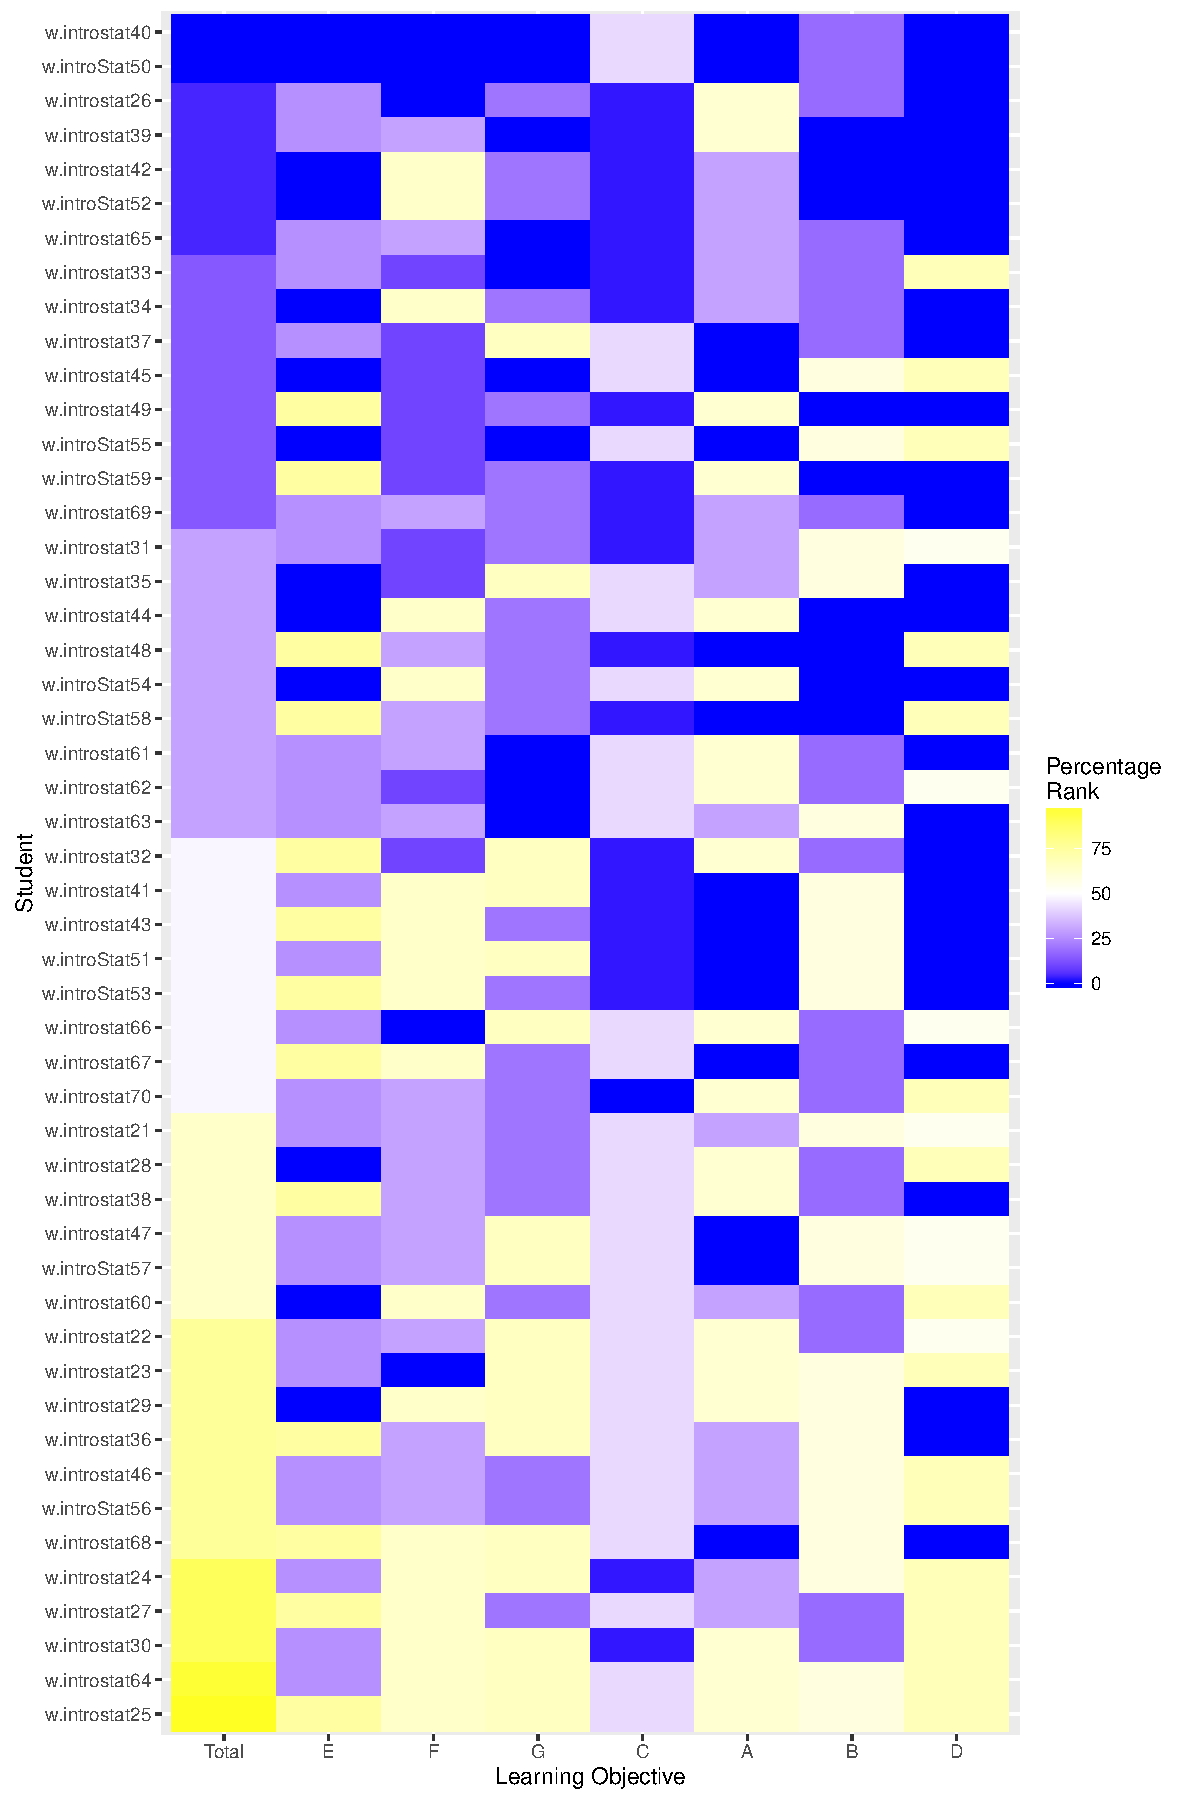
\includegraphics[width=0.99\linewidth]{Topic06_AB_tile_student_rank}
\par\end{centering}
\caption{\label{fig:LearningObj_rank}Heat map of the student ranks. Blue represents the top rank, while yellow means the bottom.}
\end{wrapfigure}\par\end{center}


\clearpage
\newpage{}
\section{Summary of Questions}

\marginnote{

 The z-score for a particular observation is z = 1.5. This means the observation is



*a. 1.5 standard deviations above the mean.



b. 1.5 standard deviations below the mean.



c. 1.5 units above the mean.



d. 1.5 units below the mean. 

}\pdfbookmark[2]{T06.A.A.04.1.1.MC.1}{T06.A.A.04.1.1.MC.1} (1) Question "T06.A.A.04.1.1.MC.1" is given on the right. This question was selected from the question set with a frequency of 0.25. The question was administered to 10 out of the total of 50 students. The average score was 0.4 out of 1.

 (Back to the question summary Table \ref{tab:summary_question}.)

\begin{center} 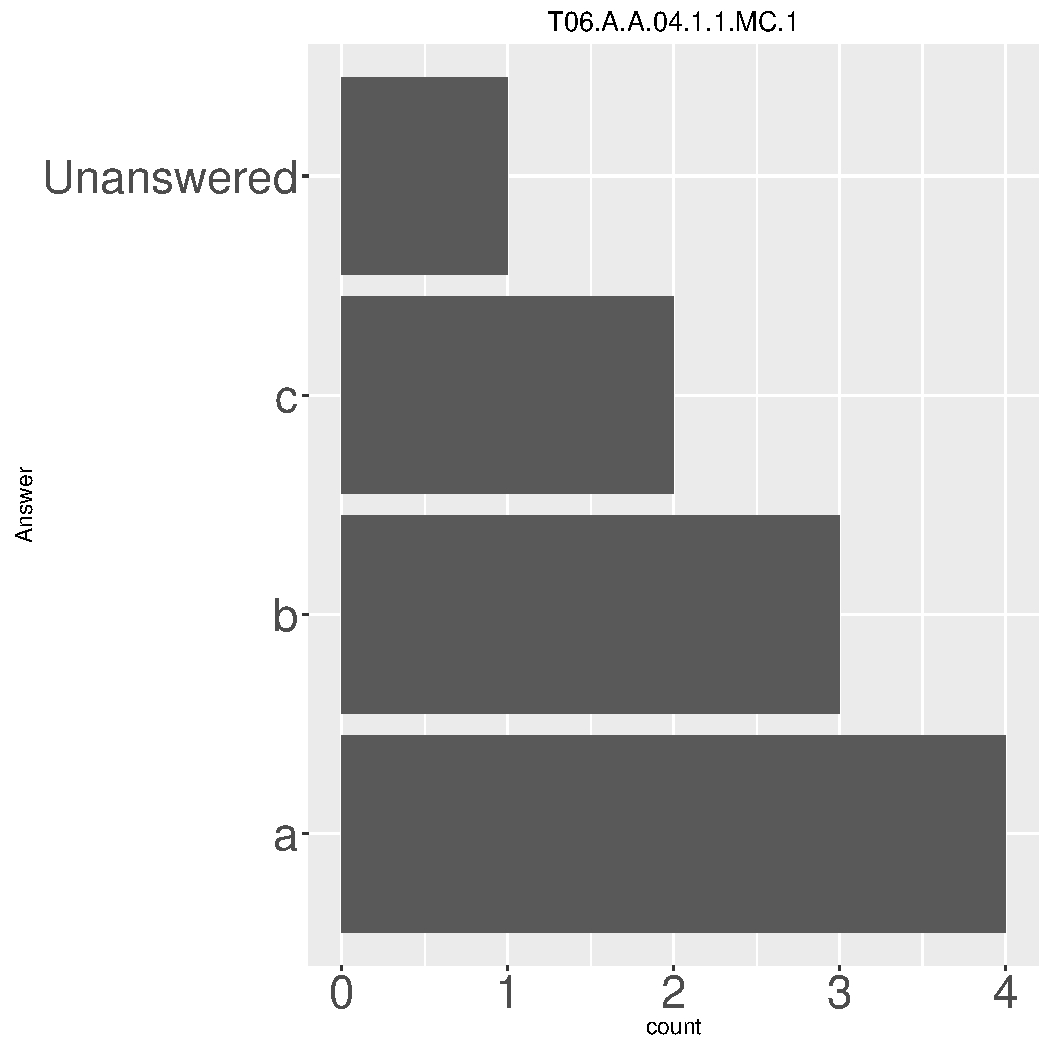
\includegraphics[width=.45\linewidth]{Topic06_AB_1_answer} 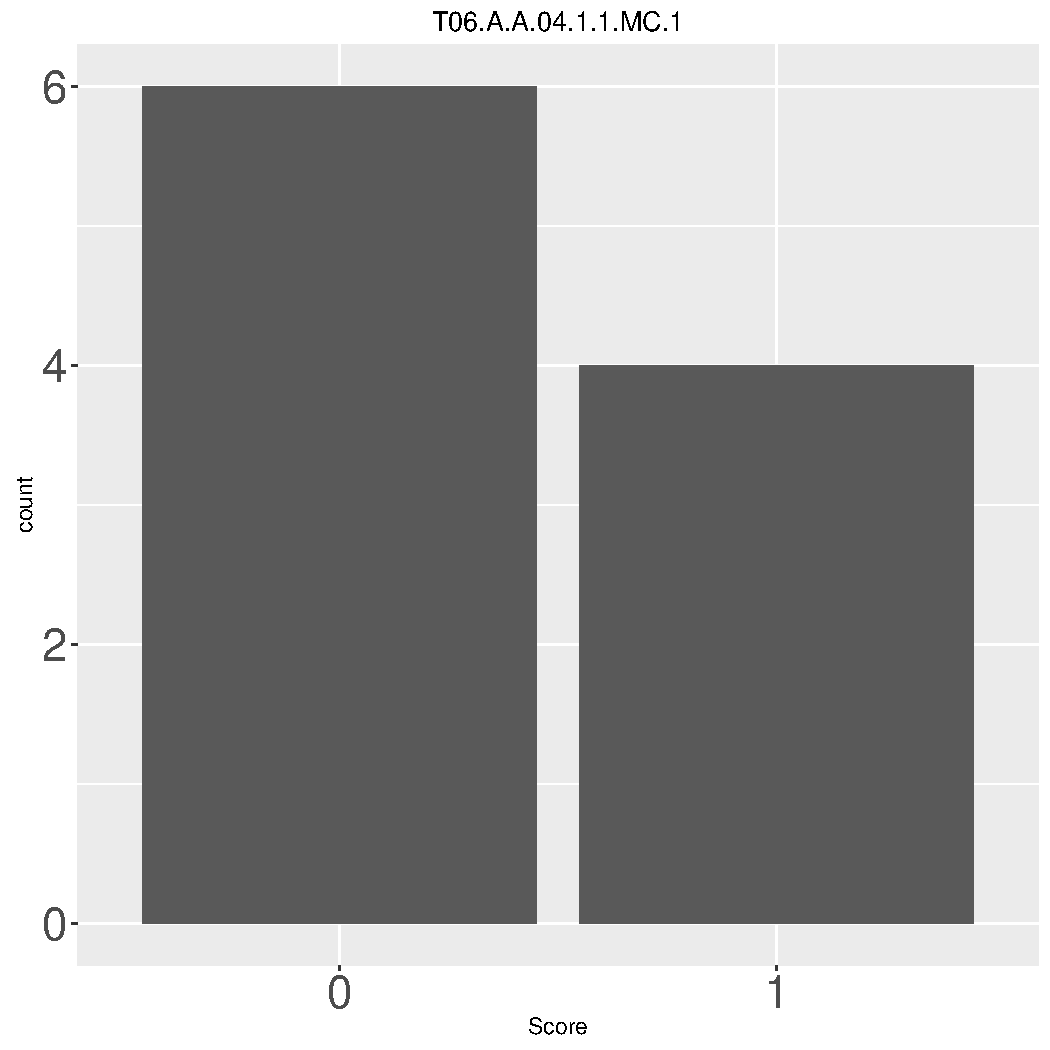
\includegraphics[width=.45\linewidth]{Topic06_AB_1_score} \end{center} 

\begin{center}% latex table generated in R 3.2.2 by xtable 1.8-0 package
% Thu Jan 21 00:33:17 2016
\begin{tabular}{lr}
  \hline
Answer & Count \\ 
  \hline
a &   4 \\ 
  b &   3 \\ 
  c &   2 \\ 
  Unanswered &   1 \\ 
   \hline
\end{tabular}
~~~~~~~~% latex table generated in R 3.2.2 by xtable 1.8-0 package
% Thu Jan 21 00:33:17 2016
\begin{tabular}{lr}
  \hline
Summary & Value \\ 
  \hline
Mean & 0.40 \\ 
  Std.dev & 0.52 \\ 
  Min & 0.00 \\ 
  Median & 0.00 \\ 
  Max & 1.00 \\ 
   \hline
\end{tabular}
\end{center}\newpage\marginnote{

 The z-score for a particular observation is z = 0.4. This means the observation is



*a. 0.4 standard deviations above the mean.



b. 0.4 standard deviations below the mean.



c. 0.4 units above the mean.



d. 0.4 units below the mean. 

}\pdfbookmark[2]{T06.A.A.04.1.1.MC.2}{T06.A.A.04.1.1.MC.2} (2) Question "T06.A.A.04.1.1.MC.2" is given on the right. This question was selected from the question set with a frequency of 0.25. The question was administered to 13 out of the total of 50 students. The average score was 0.46 out of 1.

 (Back to the question summary Table \ref{tab:summary_question}.)

\begin{center} 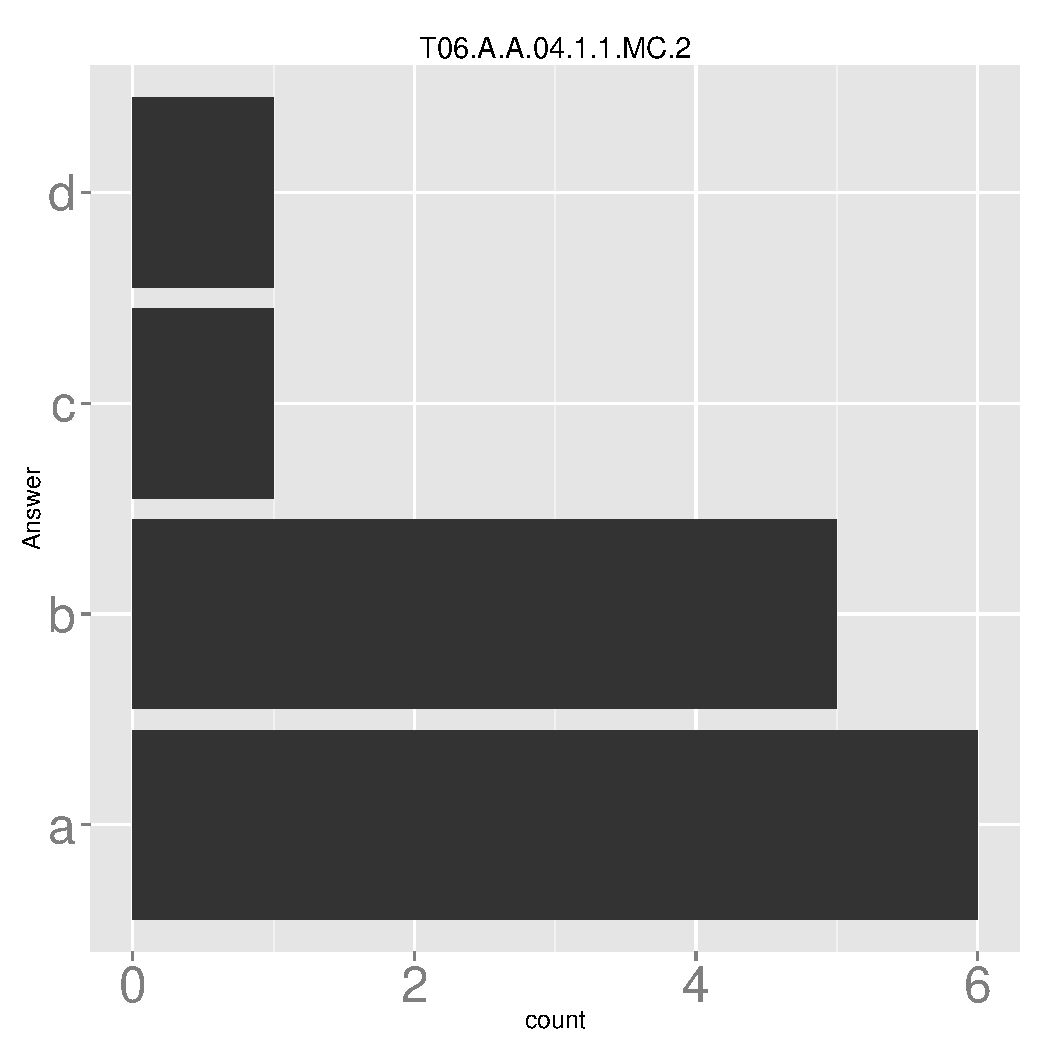
\includegraphics[width=.45\linewidth]{Topic06_AB_2_answer} 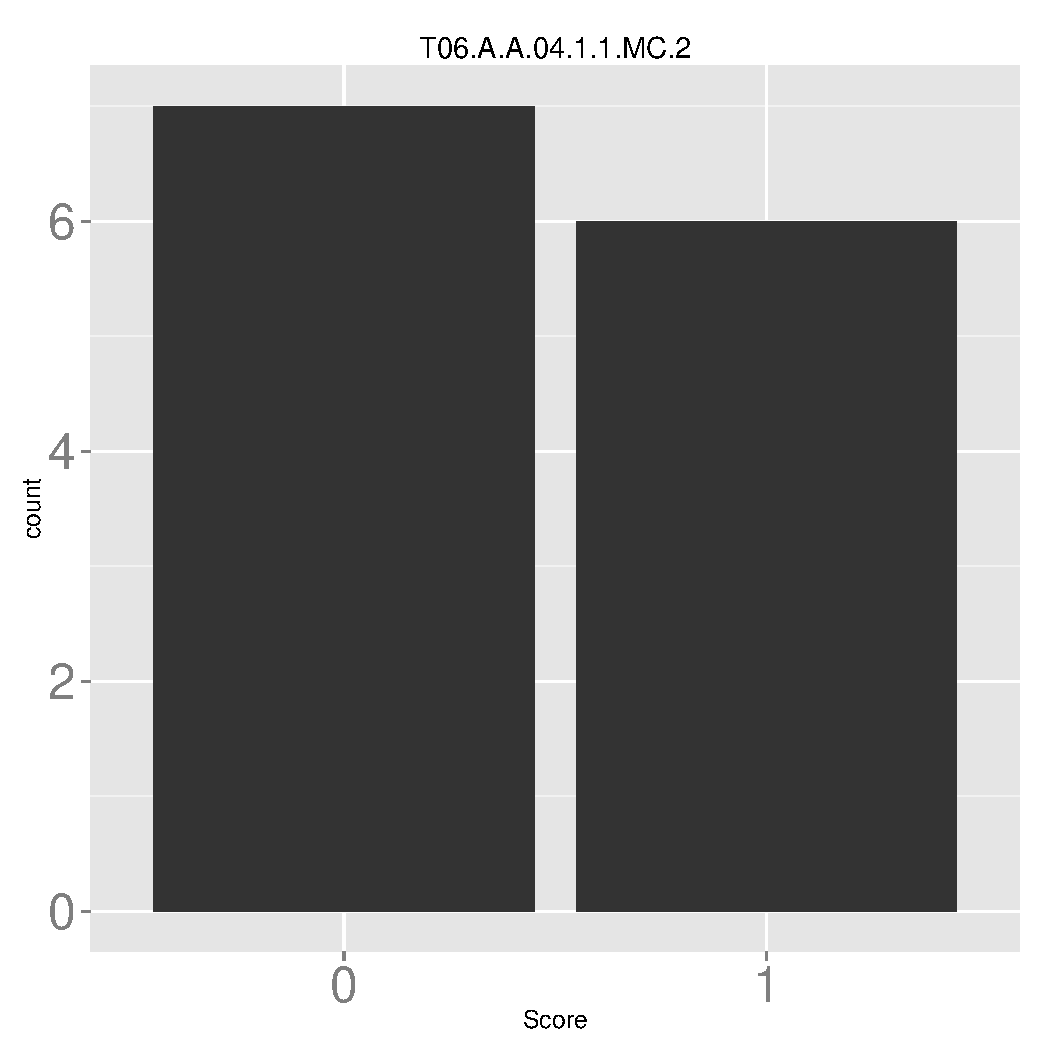
\includegraphics[width=.45\linewidth]{Topic06_AB_2_score} \end{center} 

\begin{center}% latex table generated in R 3.2.2 by xtable 1.8-0 package
% Thu Jan 21 00:33:18 2016
\begin{tabular}{lr}
  \hline
Answer & Count \\ 
  \hline
a &   6 \\ 
  b &   5 \\ 
  c &   1 \\ 
  d &   1 \\ 
   \hline
\end{tabular}
~~~~~~~~% latex table generated in R 3.2.2 by xtable 1.8-0 package
% Thu Jan 21 00:33:18 2016
\begin{tabular}{lr}
  \hline
Summary & Value \\ 
  \hline
Mean & 0.46 \\ 
  Std.dev & 0.52 \\ 
  Min & 0.00 \\ 
  Median & 0.00 \\ 
  Max & 1.00 \\ 
   \hline
\end{tabular}
\end{center}\newpage\marginnote{

 The z-score for a particular observation is z = 2.3. This means the observation is



*a. 2.3 standard deviations above the mean.



b. 2.3 standard deviations below the mean.



c. 2.3 units above the mean.



d. 2.3 units below the mean. 

}\pdfbookmark[2]{T06.A.A.04.1.1.MC.3}{T06.A.A.04.1.1.MC.3} (3) Question "T06.A.A.04.1.1.MC.3" is given on the right. This question was selected from the question set with a frequency of 0.25. The question was administered to 10 out of the total of 50 students. The average score was 0.3 out of 1.

 (Back to the question summary Table \ref{tab:summary_question}.)

\begin{center} 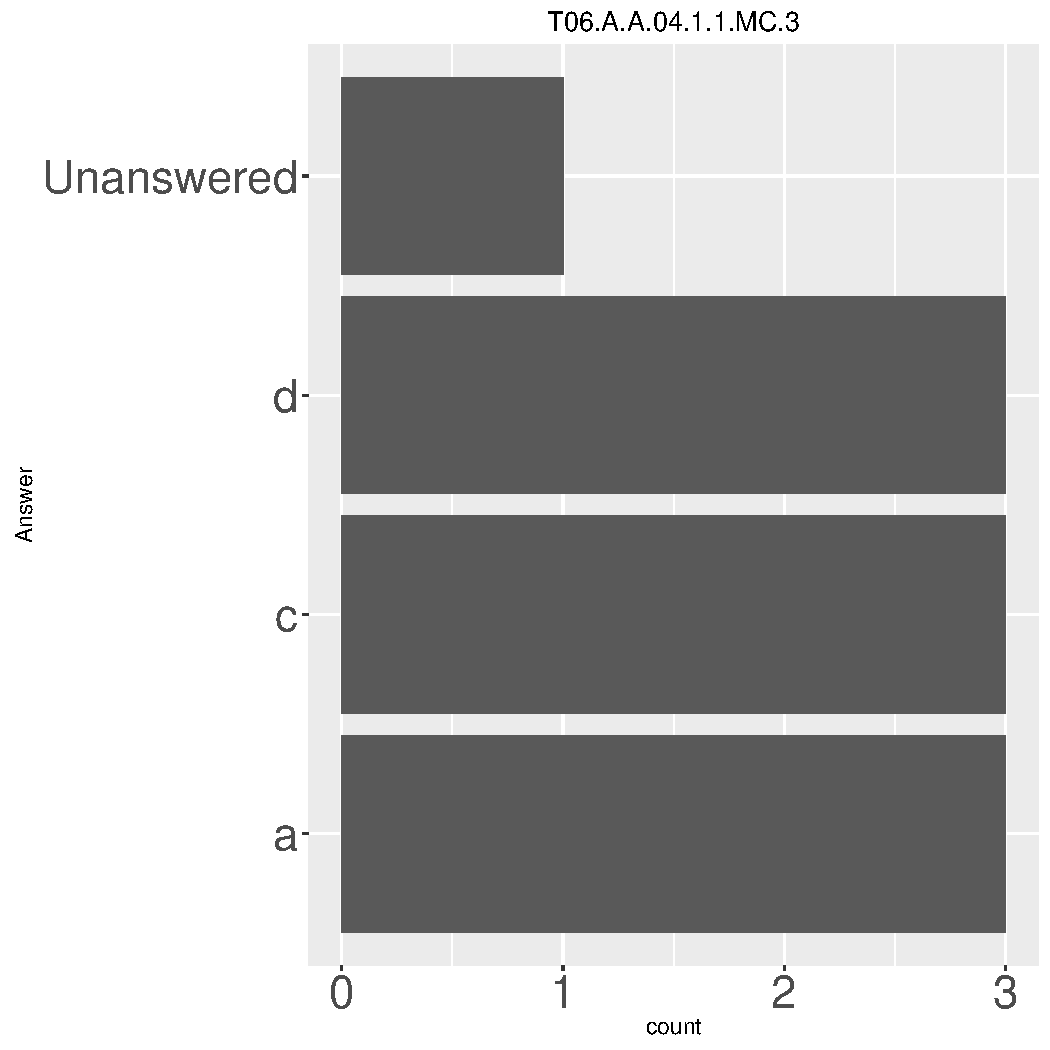
\includegraphics[width=.45\linewidth]{Topic06_AB_3_answer} 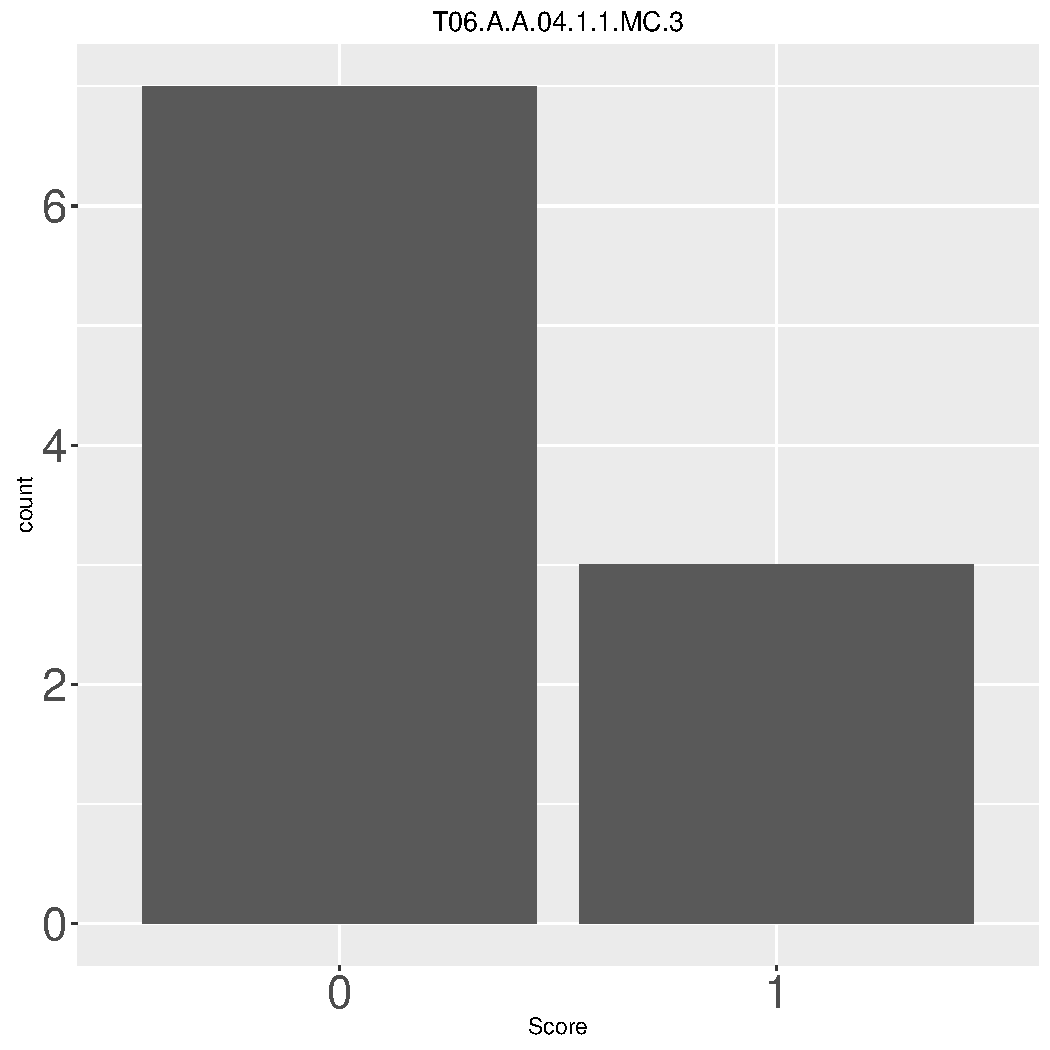
\includegraphics[width=.45\linewidth]{Topic06_AB_3_score} \end{center} 

\begin{center}% latex table generated in R 3.2.2 by xtable 1.8-0 package
% Thu Jan 21 00:33:19 2016
\begin{tabular}{lr}
  \hline
Answer & Count \\ 
  \hline
a &   3 \\ 
  c &   3 \\ 
  d &   3 \\ 
  Unanswered &   1 \\ 
   \hline
\end{tabular}
~~~~~~~~% latex table generated in R 3.2.2 by xtable 1.8-0 package
% Thu Jan 21 00:33:19 2016
\begin{tabular}{lr}
  \hline
Summary & Value \\ 
  \hline
Mean & 0.30 \\ 
  Std.dev & 0.48 \\ 
  Min & 0.00 \\ 
  Median & 0.00 \\ 
  Max & 1.00 \\ 
   \hline
\end{tabular}
\end{center}\newpage\marginnote{

 The z-score for a particular observation is z = 3.4. This means the observation is



*a. 3.4 standard deviations above the mean.



b. 3.4 standard deviations below the mean.



c. 3.4 units above the mean.



d. 3.4 units below the mean. 

}\pdfbookmark[2]{T06.A.A.04.1.1.MC.4}{T06.A.A.04.1.1.MC.4} (4) Question "T06.A.A.04.1.1.MC.4" is given on the right. This question was selected from the question set with a frequency of 0.25. The question was administered to 17 out of the total of 50 students. The average score was 0.53 out of 1.

 (Back to the question summary Table \ref{tab:summary_question}.)

\begin{center} 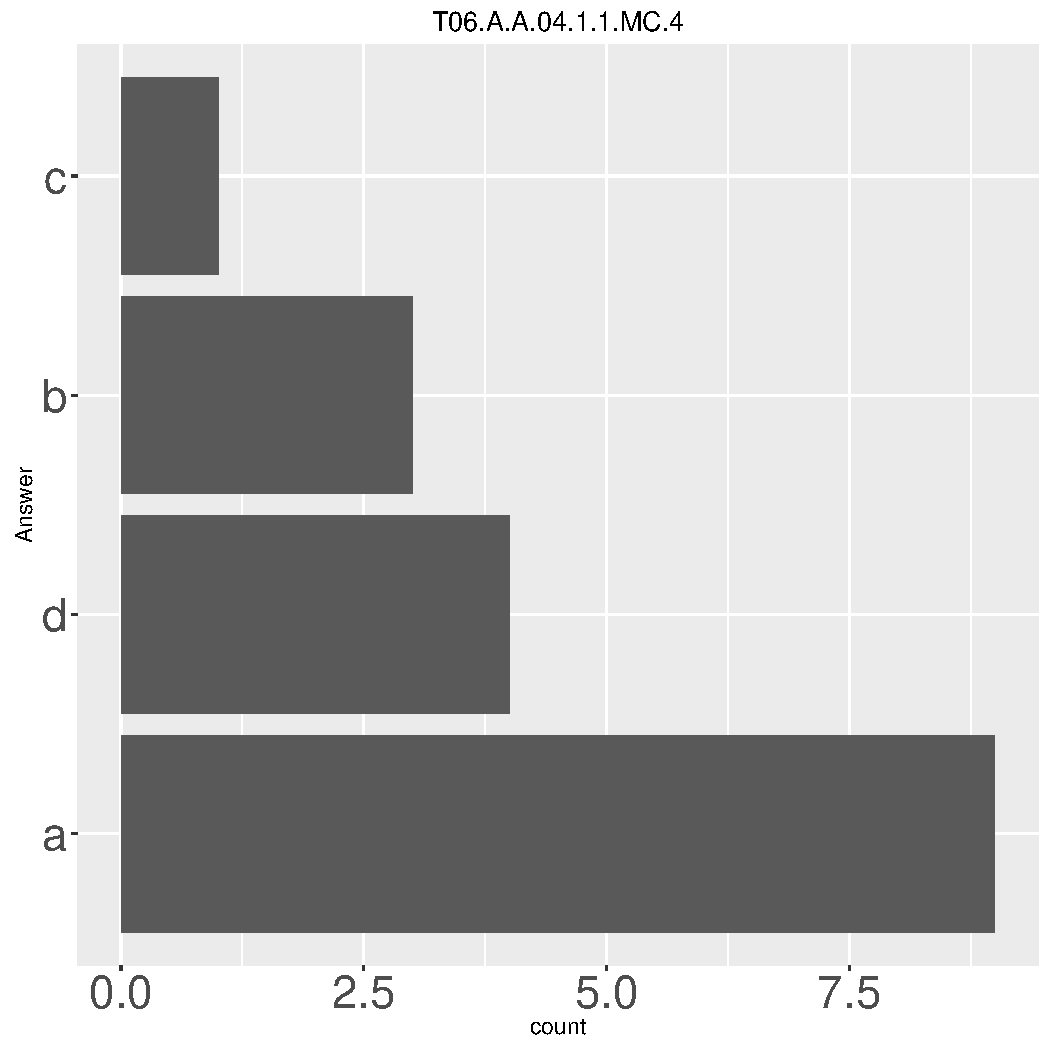
\includegraphics[width=.45\linewidth]{Topic06_AB_4_answer} 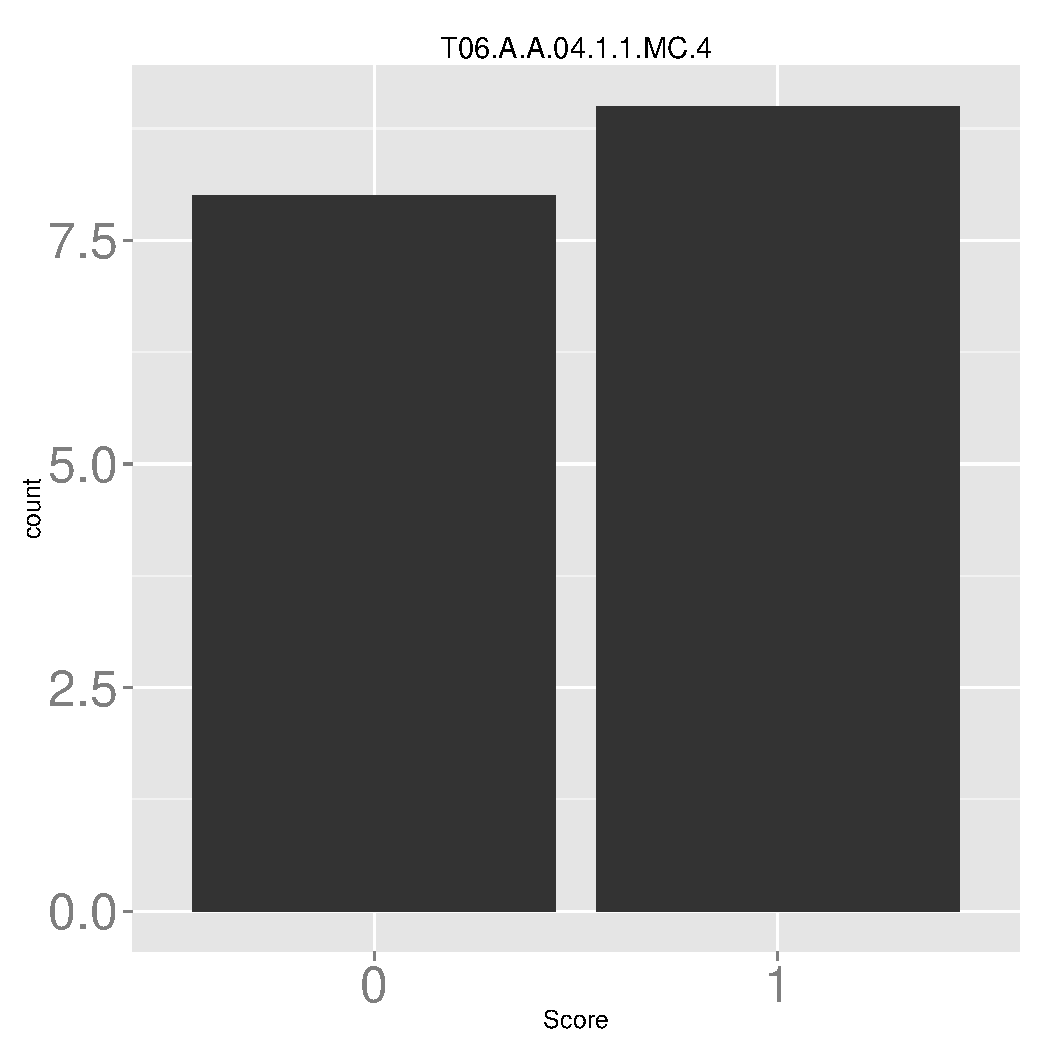
\includegraphics[width=.45\linewidth]{Topic06_AB_4_score} \end{center} 

\begin{center}% latex table generated in R 3.2.2 by xtable 1.8-0 package
% Thu Jan 21 00:33:19 2016
\begin{tabular}{lr}
  \hline
Answer & Count \\ 
  \hline
a &   9 \\ 
  d &   4 \\ 
  b &   3 \\ 
  c &   1 \\ 
   \hline
\end{tabular}
~~~~~~~~% latex table generated in R 3.2.2 by xtable 1.8-0 package
% Thu Jan 21 00:33:19 2016
\begin{tabular}{lr}
  \hline
Summary & Value \\ 
  \hline
Mean & 0.53 \\ 
  Std.dev & 0.51 \\ 
  Min & 0.00 \\ 
  Median & 1.00 \\ 
  Max & 1.00 \\ 
   \hline
\end{tabular}
\end{center}\newpage\marginnote{

 The z-score for a particular observation is z = -1.2. This means the observation is



a. 1.2 standard deviations above the mean.



*b. 1.2 standard deviations below the mean.



c. 1.2 units above the mean.



d. 1.2 units below the mean. 

}\pdfbookmark[2]{T06.A.B.04.1.1.MC.1}{T06.A.B.04.1.1.MC.1} (5) Question "T06.A.B.04.1.1.MC.1" is given on the right. This question was selected from the question set with a frequency of 0.25. The question was administered to 14 out of the total of 50 students. The average score was 0.43 out of 1.

 (Back to the question summary Table \ref{tab:summary_question}.)

\begin{center} 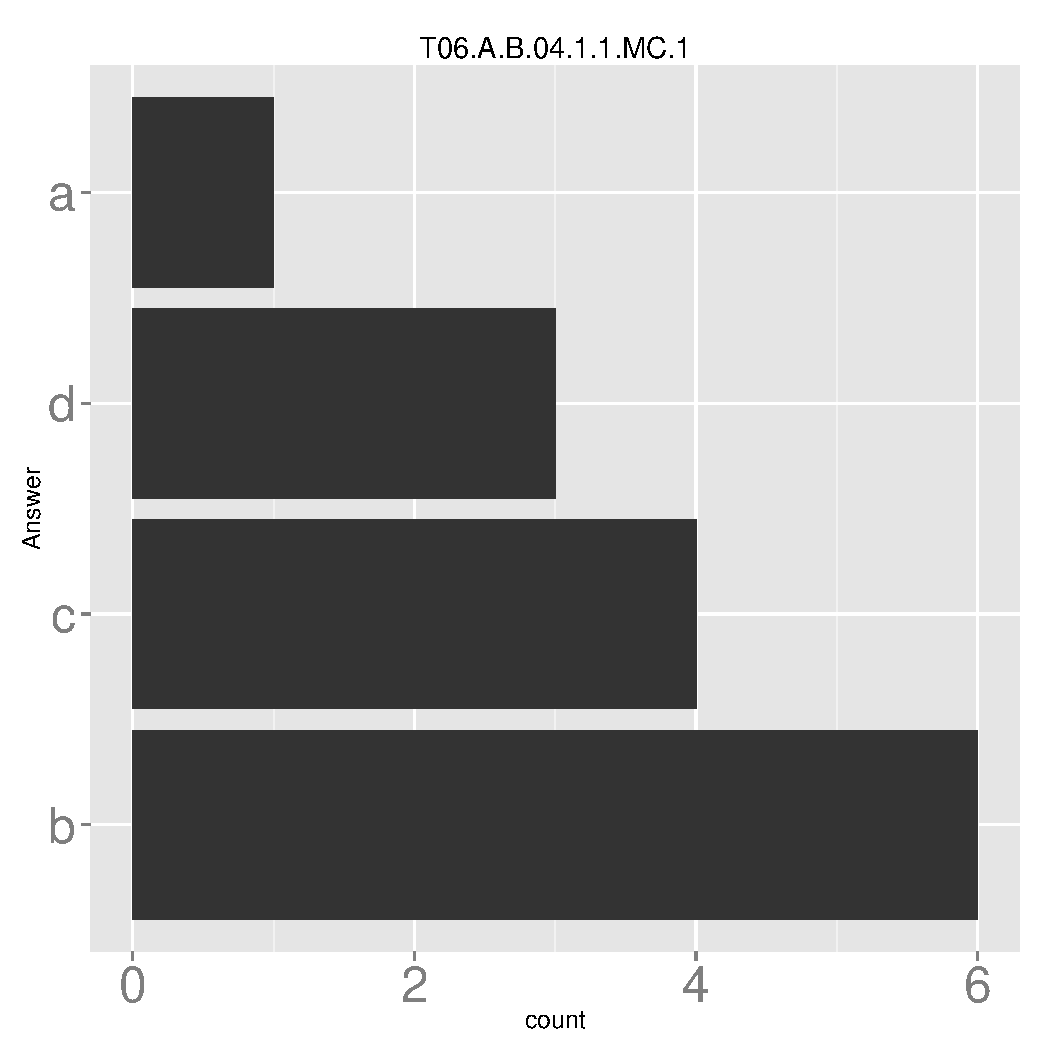
\includegraphics[width=.45\linewidth]{Topic06_AB_5_answer} 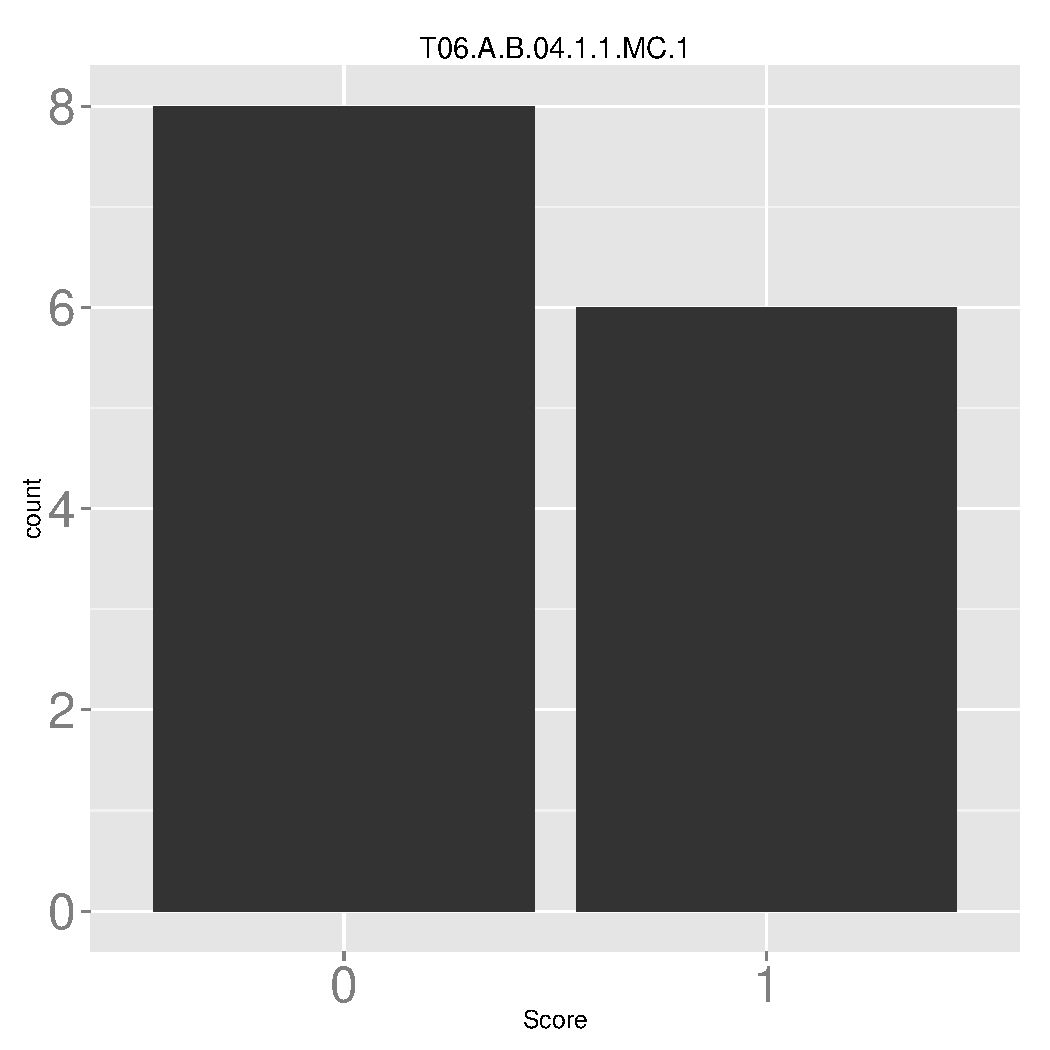
\includegraphics[width=.45\linewidth]{Topic06_AB_5_score} \end{center} 

\begin{center}% latex table generated in R 3.2.2 by xtable 1.8-0 package
% Thu Jan 21 00:33:20 2016
\begin{tabular}{lr}
  \hline
Answer & Count \\ 
  \hline
b &   6 \\ 
  c &   4 \\ 
  d &   3 \\ 
  a &   1 \\ 
   \hline
\end{tabular}
~~~~~~~~% latex table generated in R 3.2.2 by xtable 1.8-0 package
% Thu Jan 21 00:33:20 2016
\begin{tabular}{lr}
  \hline
Summary & Value \\ 
  \hline
Mean & 0.43 \\ 
  Std.dev & 0.51 \\ 
  Min & 0.00 \\ 
  Median & 0.00 \\ 
  Max & 1.00 \\ 
   \hline
\end{tabular}
\end{center}\newpage\marginnote{

 The z-score for a particular observation is z = -0.8. This means the observation is



a. 0.8 standard deviations above the mean.



*b. 0.8 standard deviations below the mean.



c. 0.8 units above the mean.



d. 0.8 units below the mean. 

}\pdfbookmark[2]{T06.A.B.04.1.1.MC.2}{T06.A.B.04.1.1.MC.2} (6) Question "T06.A.B.04.1.1.MC.2" is given on the right. This question was selected from the question set with a frequency of 0.25. The question was administered to 16 out of the total of 50 students. The average score was 0.5 out of 1.

 (Back to the question summary Table \ref{tab:summary_question}.)

\begin{center} 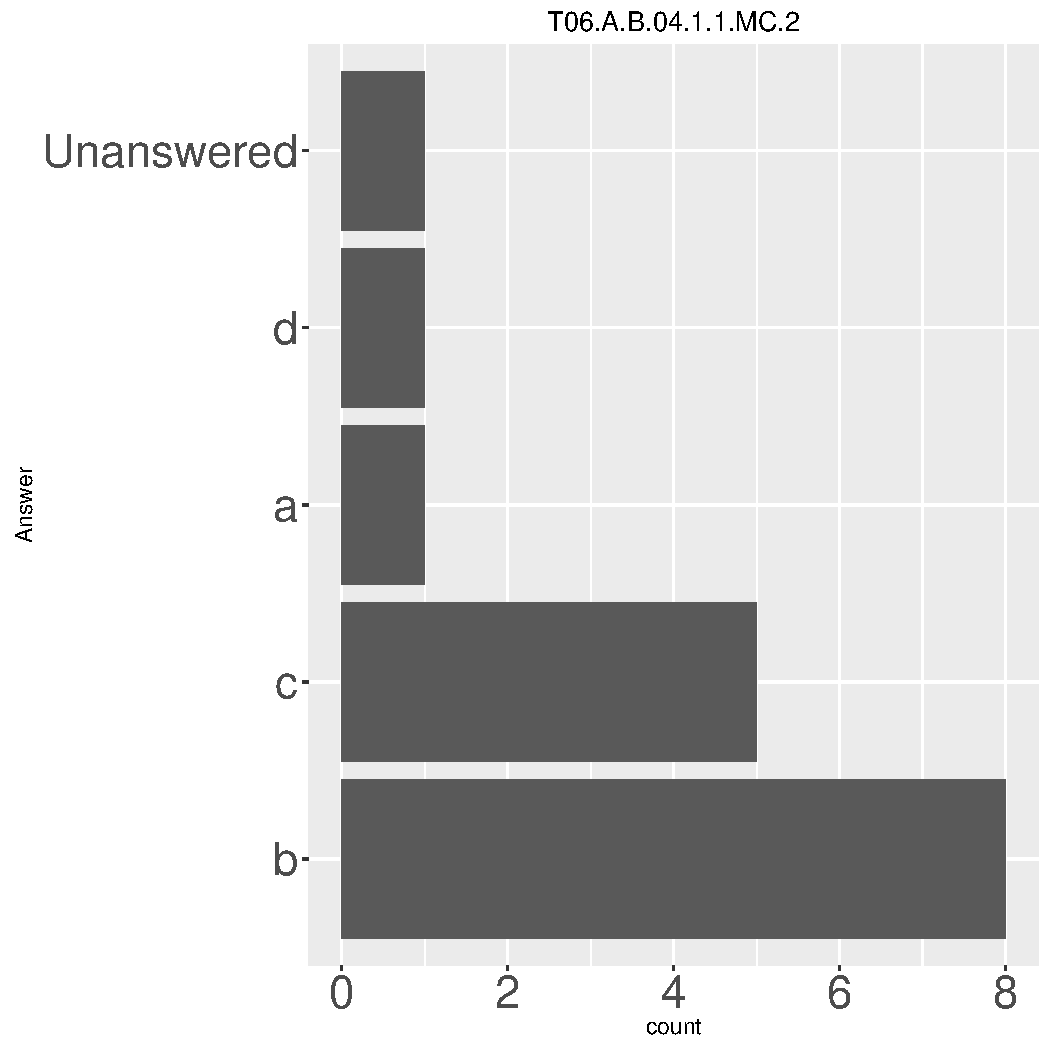
\includegraphics[width=.45\linewidth]{Topic06_AB_6_answer} 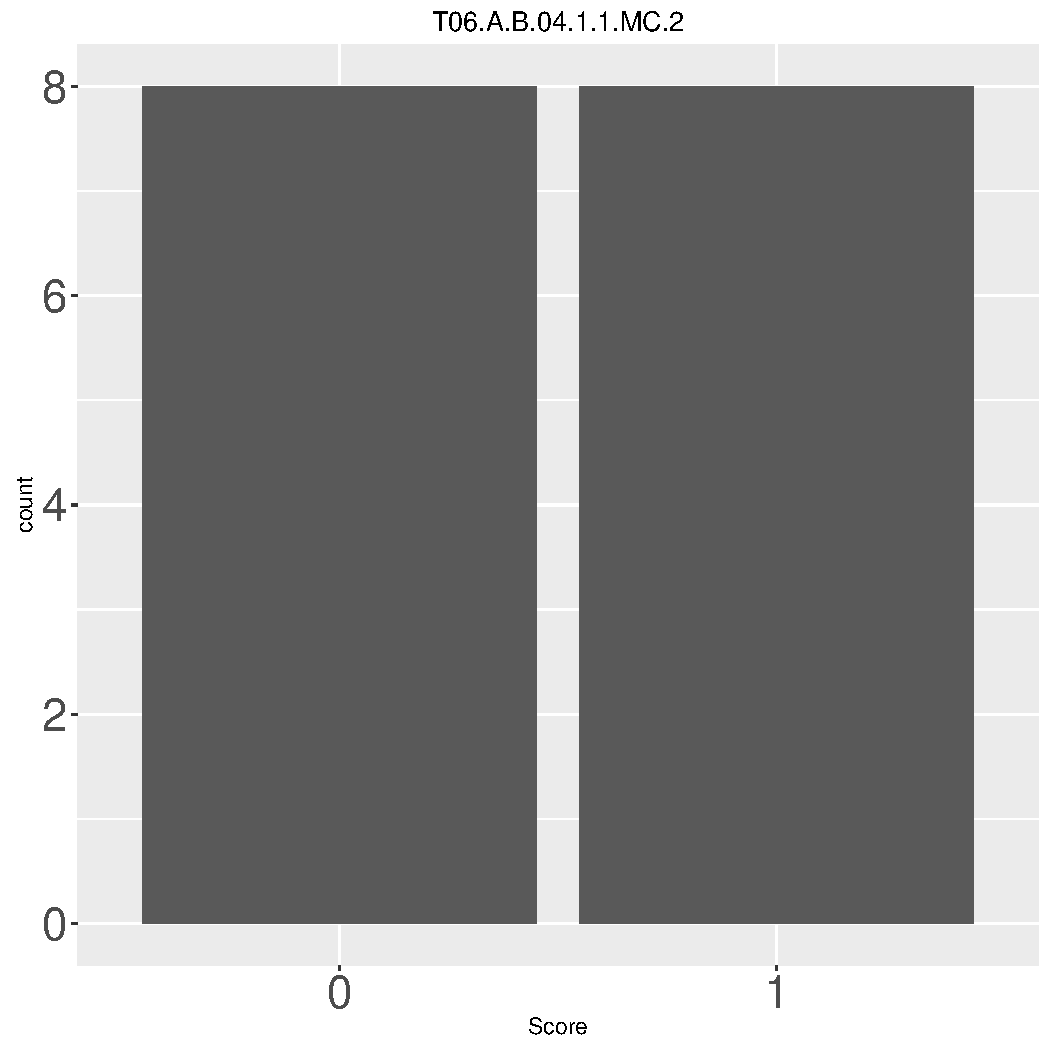
\includegraphics[width=.45\linewidth]{Topic06_AB_6_score} \end{center} 

\begin{center}% latex table generated in R 3.2.2 by xtable 1.8-0 package
% Thu Jan 21 00:33:21 2016
\begin{tabular}{lr}
  \hline
Answer & Count \\ 
  \hline
b &   8 \\ 
  c &   5 \\ 
  a &   1 \\ 
  d &   1 \\ 
  Unanswered &   1 \\ 
   \hline
\end{tabular}
~~~~~~~~% latex table generated in R 3.2.2 by xtable 1.8-0 package
% Thu Jan 21 00:33:21 2016
\begin{tabular}{lr}
  \hline
Summary & Value \\ 
  \hline
Mean & 0.50 \\ 
  Std.dev & 0.52 \\ 
  Min & 0.00 \\ 
  Median & 0.50 \\ 
  Max & 1.00 \\ 
   \hline
\end{tabular}
\end{center}\newpage\marginnote{

 The z-score for a particular observation is z = -2.7. This means the observation is



a. 2.7 standard deviations above the mean.



*b. 2.7 standard deviations below the mean.



c. 2.7 units above the mean.



d. 2.7 units below the mean. 

}\pdfbookmark[2]{T06.A.B.04.1.1.MC.3}{T06.A.B.04.1.1.MC.3} (7) Question "T06.A.B.04.1.1.MC.3" is given on the right. This question was selected from the question set with a frequency of 0.25. The question was administered to 8 out of the total of 50 students. The average score was 0.25 out of 1.

 (Back to the question summary Table \ref{tab:summary_question}.)

\begin{center} 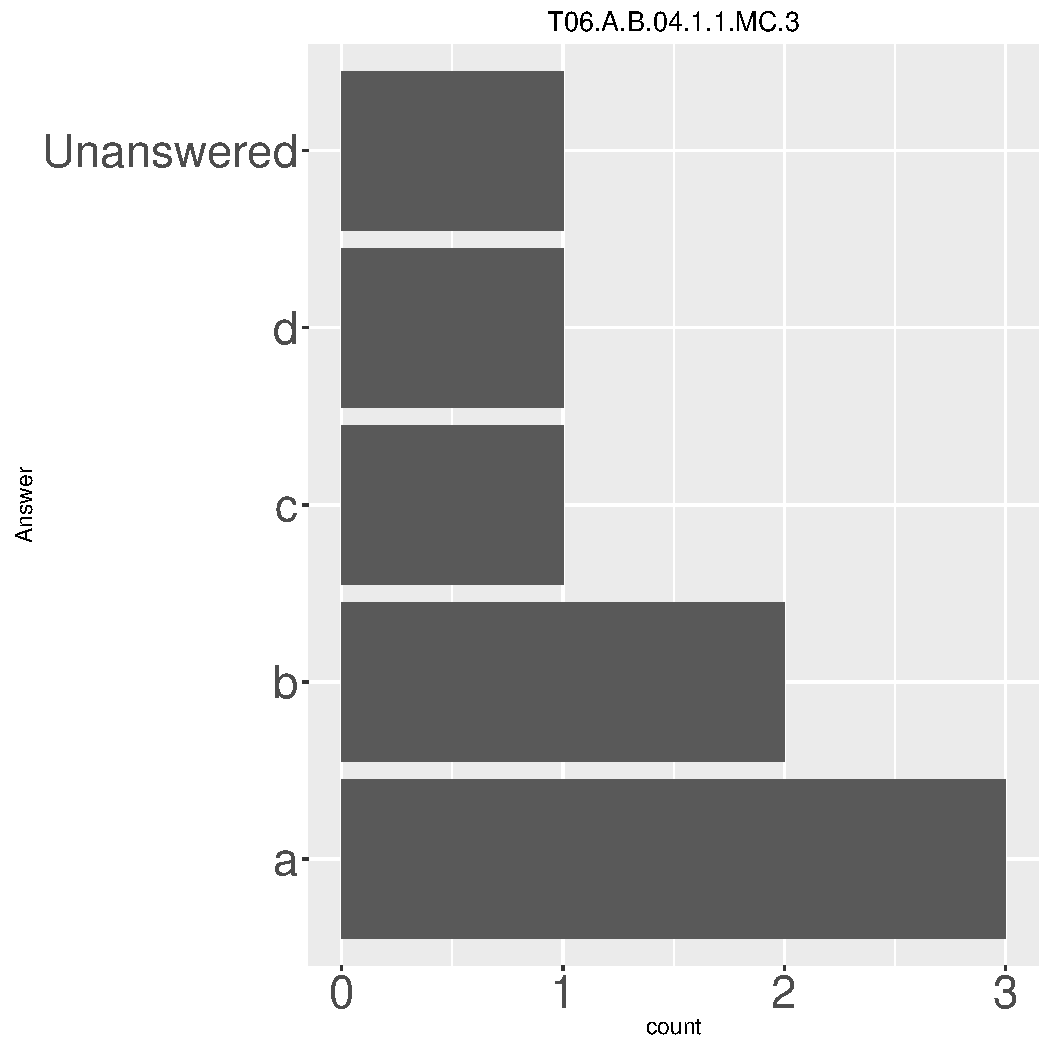
\includegraphics[width=.45\linewidth]{Topic06_AB_7_answer} 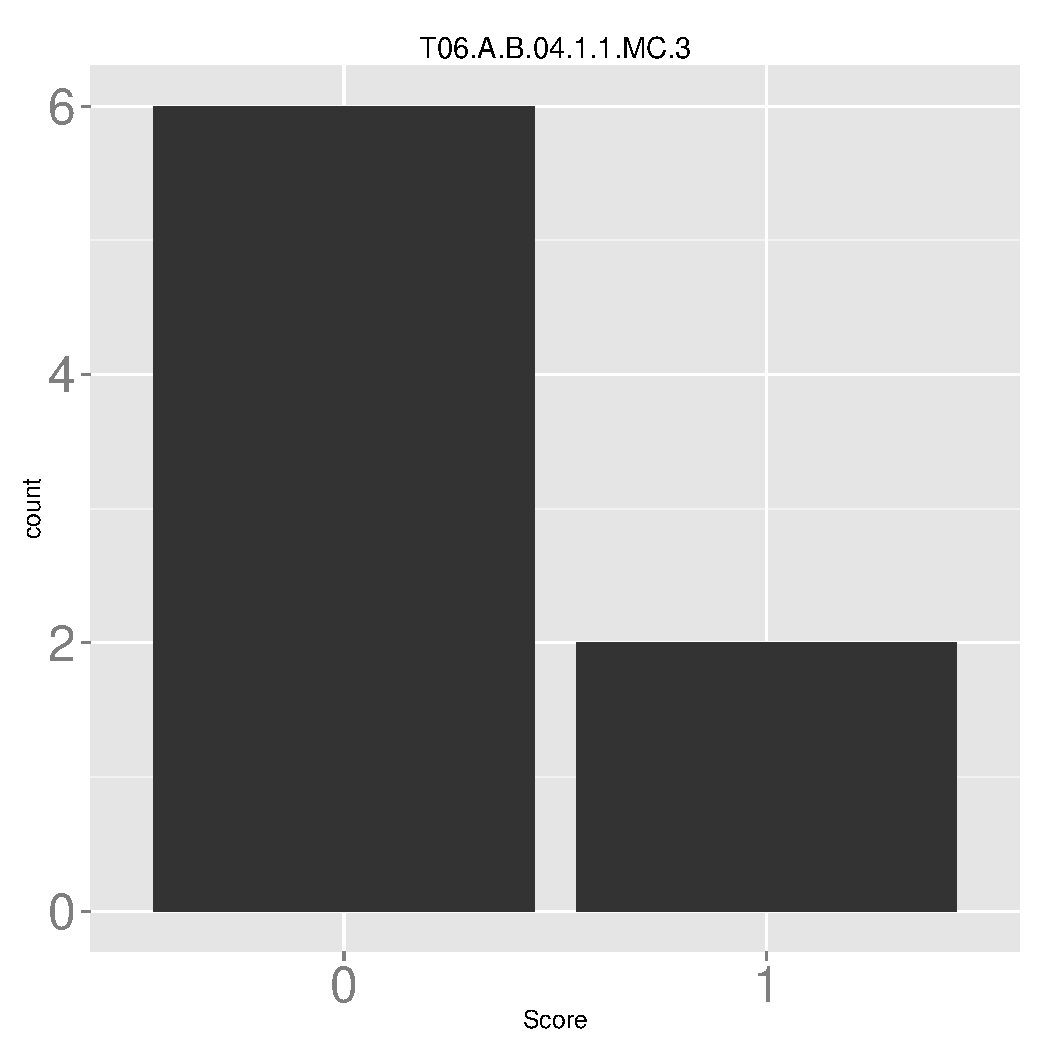
\includegraphics[width=.45\linewidth]{Topic06_AB_7_score} \end{center} 

\begin{center}% latex table generated in R 3.2.2 by xtable 1.8-0 package
% Thu Jan 21 00:33:22 2016
\begin{tabular}{lr}
  \hline
Answer & Count \\ 
  \hline
a &   3 \\ 
  b &   2 \\ 
  c &   1 \\ 
  d &   1 \\ 
  Unanswered &   1 \\ 
   \hline
\end{tabular}
~~~~~~~~% latex table generated in R 3.2.2 by xtable 1.8-0 package
% Thu Jan 21 00:33:22 2016
\begin{tabular}{lr}
  \hline
Summary & Value \\ 
  \hline
Mean & 0.25 \\ 
  Std.dev & 0.46 \\ 
  Min & 0.00 \\ 
  Median & 0.00 \\ 
  Max & 1.00 \\ 
   \hline
\end{tabular}
\end{center}\newpage\marginnote{

 The z-score for a particular observation is z = -3.1. This means the observation is



a. 3.1 standard deviations above the mean.



*b. 3.1 standard deviations below the mean.



c. 3.1 units above the mean.



d. 3.1 units below the mean. 

}\pdfbookmark[2]{T06.A.B.04.1.1.MC.4}{T06.A.B.04.1.1.MC.4} (8) Question "T06.A.B.04.1.1.MC.4" is given on the right. This question was selected from the question set with a frequency of 0.25. The question was administered to 12 out of the total of 50 students. The average score was 0.67 out of 1.

 (Back to the question summary Table \ref{tab:summary_question}.)

\begin{center} 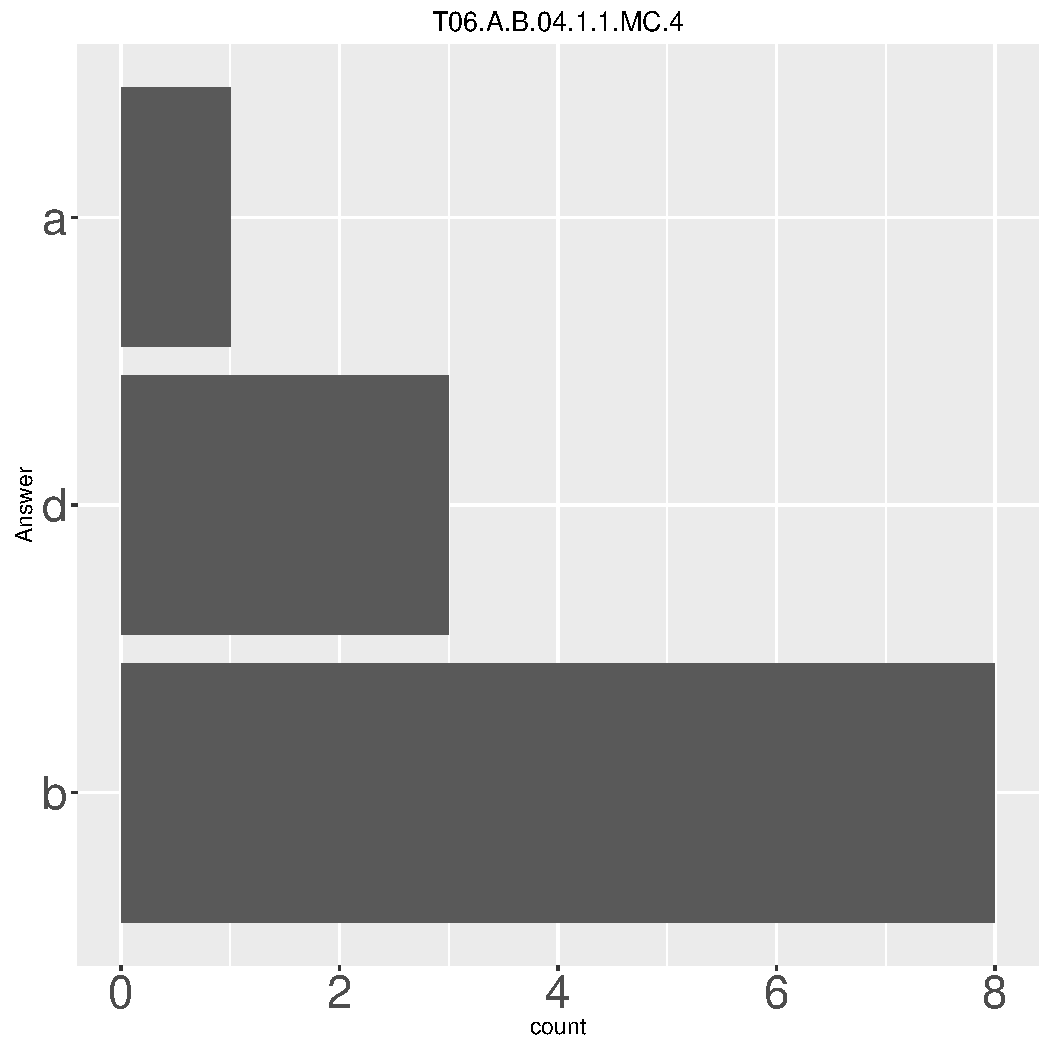
\includegraphics[width=.45\linewidth]{Topic06_AB_8_answer} 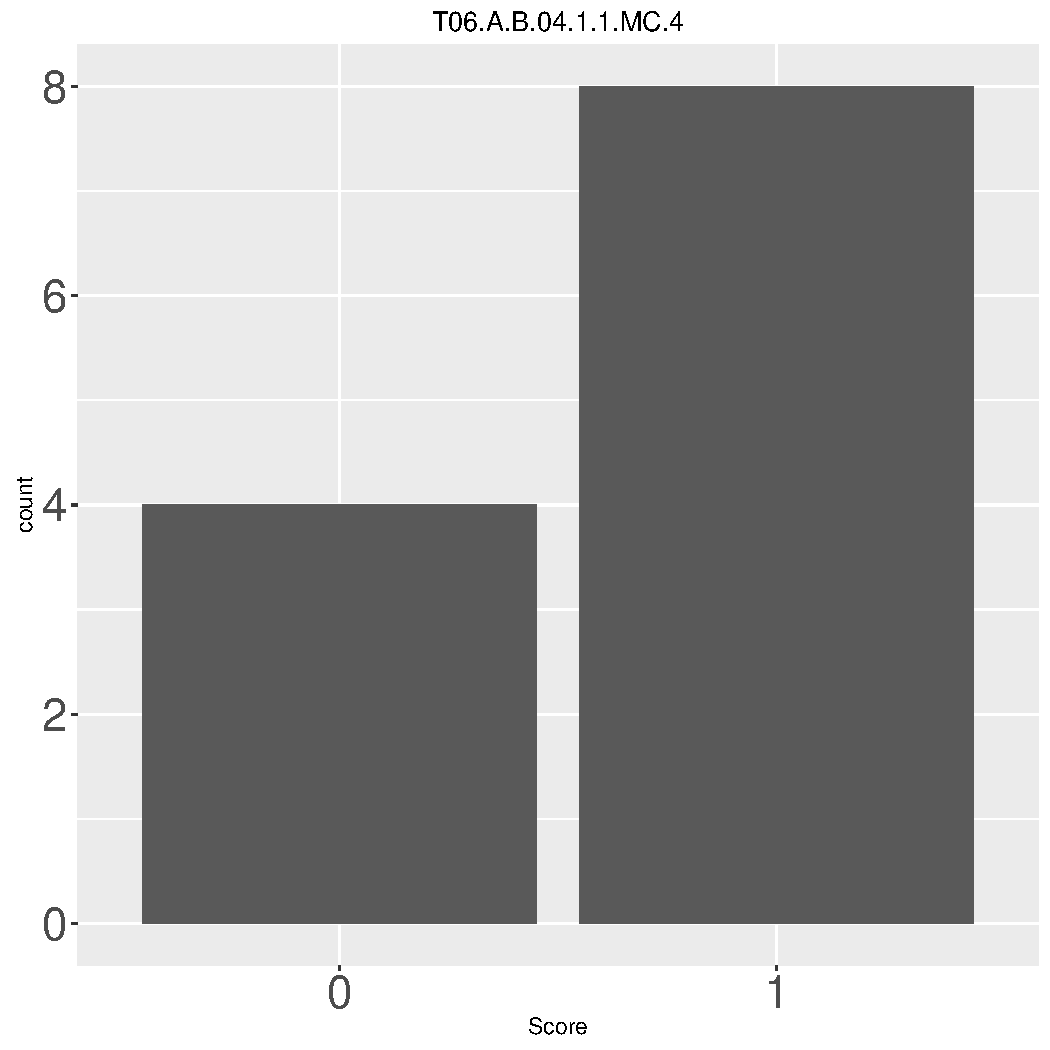
\includegraphics[width=.45\linewidth]{Topic06_AB_8_score} \end{center} 

\begin{center}% latex table generated in R 3.2.2 by xtable 1.8-0 package
% Thu Jan 21 00:33:22 2016
\begin{tabular}{lr}
  \hline
Answer & Count \\ 
  \hline
b &   8 \\ 
  d &   3 \\ 
  a &   1 \\ 
   \hline
\end{tabular}
~~~~~~~~% latex table generated in R 3.2.2 by xtable 1.8-0 package
% Thu Jan 21 00:33:22 2016
\begin{tabular}{lr}
  \hline
Summary & Value \\ 
  \hline
Mean & 0.67 \\ 
  Std.dev & 0.49 \\ 
  Min & 0.00 \\ 
  Median & 1.00 \\ 
  Max & 1.00 \\ 
   \hline
\end{tabular}
\end{center}\newpage\marginnote{

 In a sample of 25 male newborns, the mean birth weight was 3.4 kg and the standard deviation was 0.35 kg.



The z-score for a birth weight of 4.5 kg is \_\_\_\_\_\_\_\_\_\_. Round your answer to 2 decimal places.



Correct Answer(s):



a. 3.14



b. 3.15



c. 3.13 

}\pdfbookmark[2]{T06.A.C.04.1.1.FB.1}{T06.A.C.04.1.1.FB.1} (9) Question "T06.A.C.04.1.1.FB.1" is given on the right. This question was selected from the question set with a frequency of 0.25. The question was administered to 11 out of the total of 50 students. The average score was 0 out of 1.

 (Back to the question summary Table \ref{tab:summary_question}.)

\begin{center} 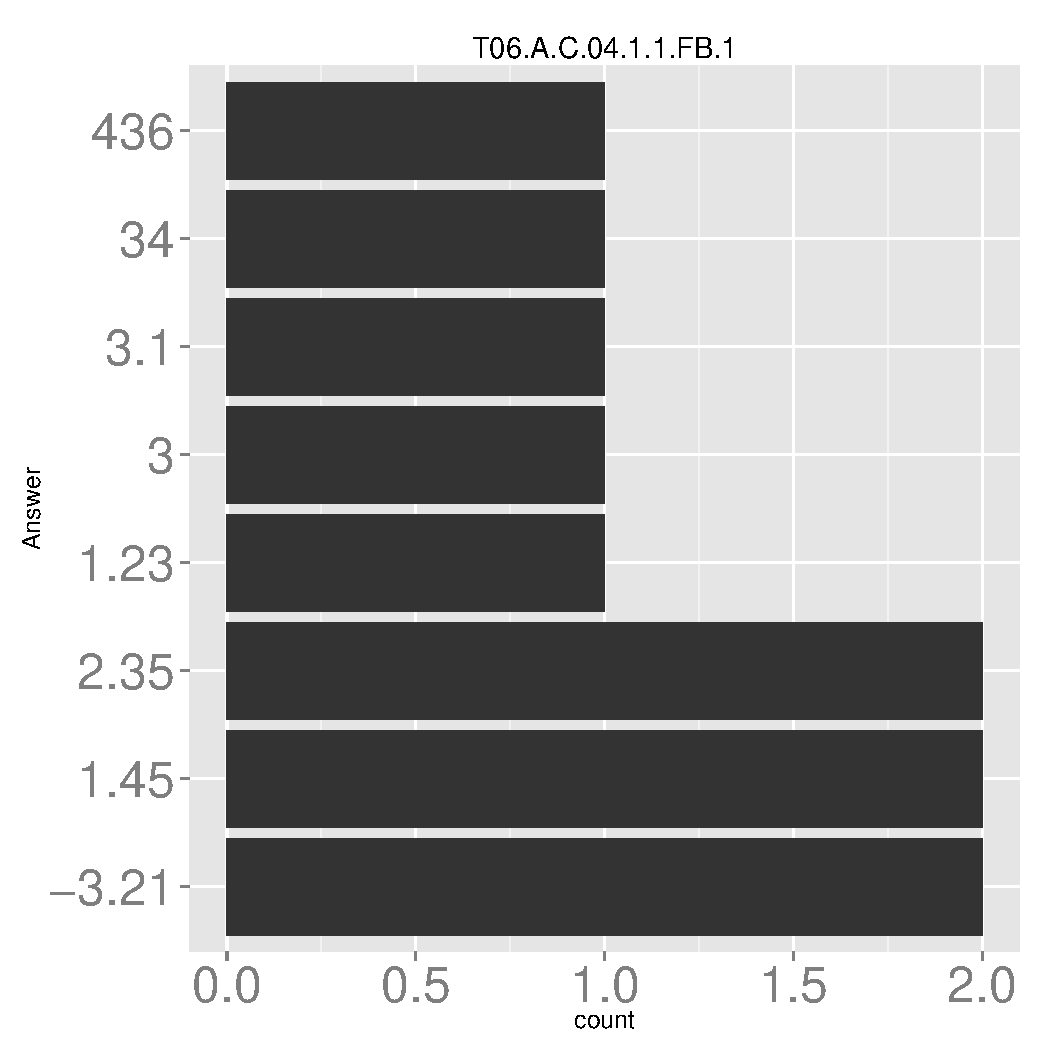
\includegraphics[width=.45\linewidth]{Topic06_AB_9_answer} 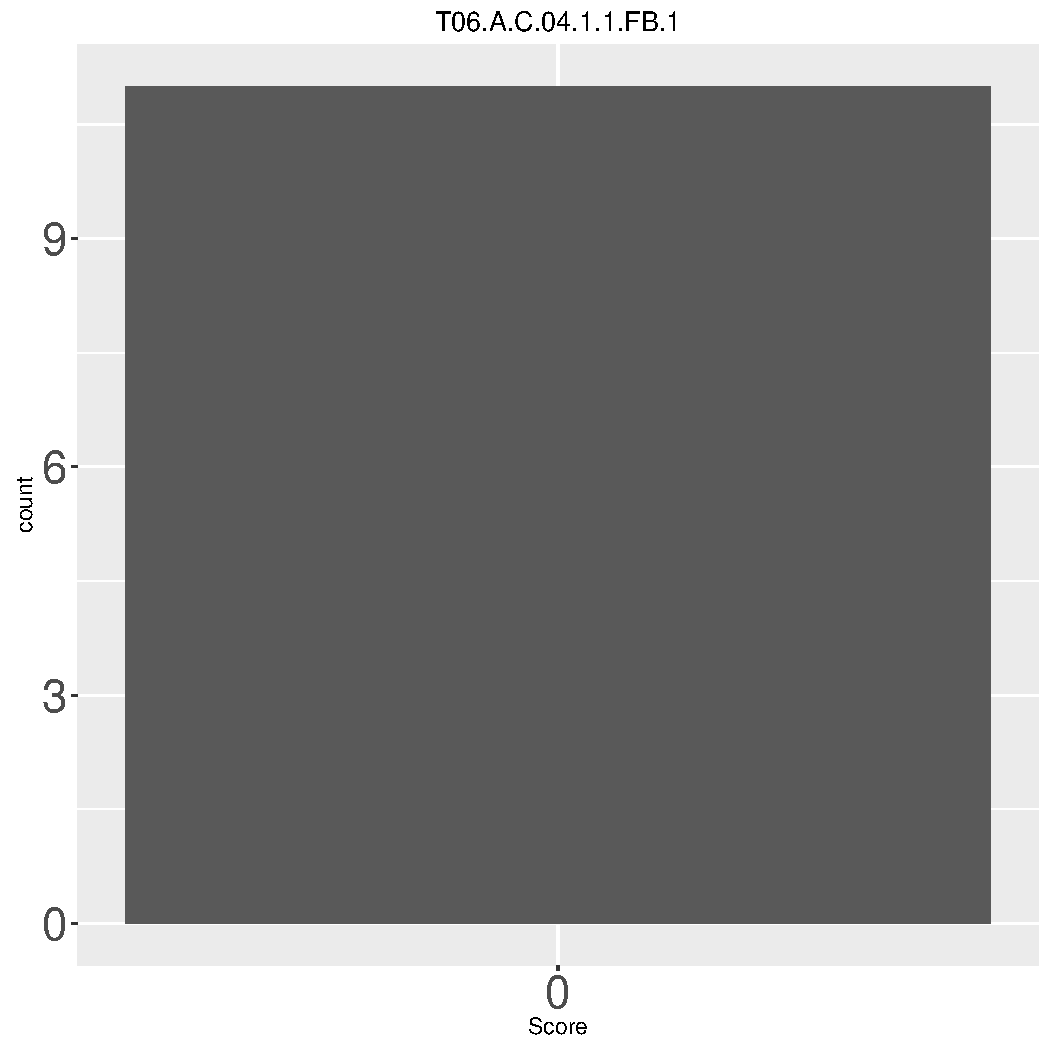
\includegraphics[width=.45\linewidth]{Topic06_AB_9_score} \end{center} 

\begin{center}% latex table generated in R 3.2.2 by xtable 1.8-0 package
% Thu Jan 21 00:33:23 2016
\begin{tabular}{lr}
  \hline
Answer & Count \\ 
  \hline
-3.21 &   2 \\ 
  1.45 &   2 \\ 
  2.35 &   2 \\ 
  1.23 &   1 \\ 
  3 &   1 \\ 
  3.1 &   1 \\ 
  34 &   1 \\ 
  436 &   1 \\ 
   \hline
\end{tabular}
~~~~~~~~% latex table generated in R 3.2.2 by xtable 1.8-0 package
% Thu Jan 21 00:33:23 2016
\begin{tabular}{lr}
  \hline
Summary & Value \\ 
  \hline
Mean & 0.00 \\ 
  Std.dev & 0.00 \\ 
  Min & 0.00 \\ 
  Median & 0.00 \\ 
  Max & 0.00 \\ 
   \hline
\end{tabular}
\end{center}\newpage\marginnote{

 In a sample of 25 male newborns, the mean birth weight was 3.4 kg and the standard deviation was 0.35 kg.



The z-score for a birth weight of 4.0 kg is \_\_\_\_\_\_\_\_\_\_. Round your answer to 2 decimal places.



Correct Answer(s):



a. 1.71



b. 1.72



c. 1.70



d. 1.7 

}\pdfbookmark[2]{T06.A.C.04.1.1.FB.2}{T06.A.C.04.1.1.FB.2} (10) Question "T06.A.C.04.1.1.FB.2" is given on the right. This question was selected from the question set with a frequency of 0.25. The question was administered to 11 out of the total of 50 students. The average score was 0 out of 1.

 (Back to the question summary Table \ref{tab:summary_question}.)

\begin{center} 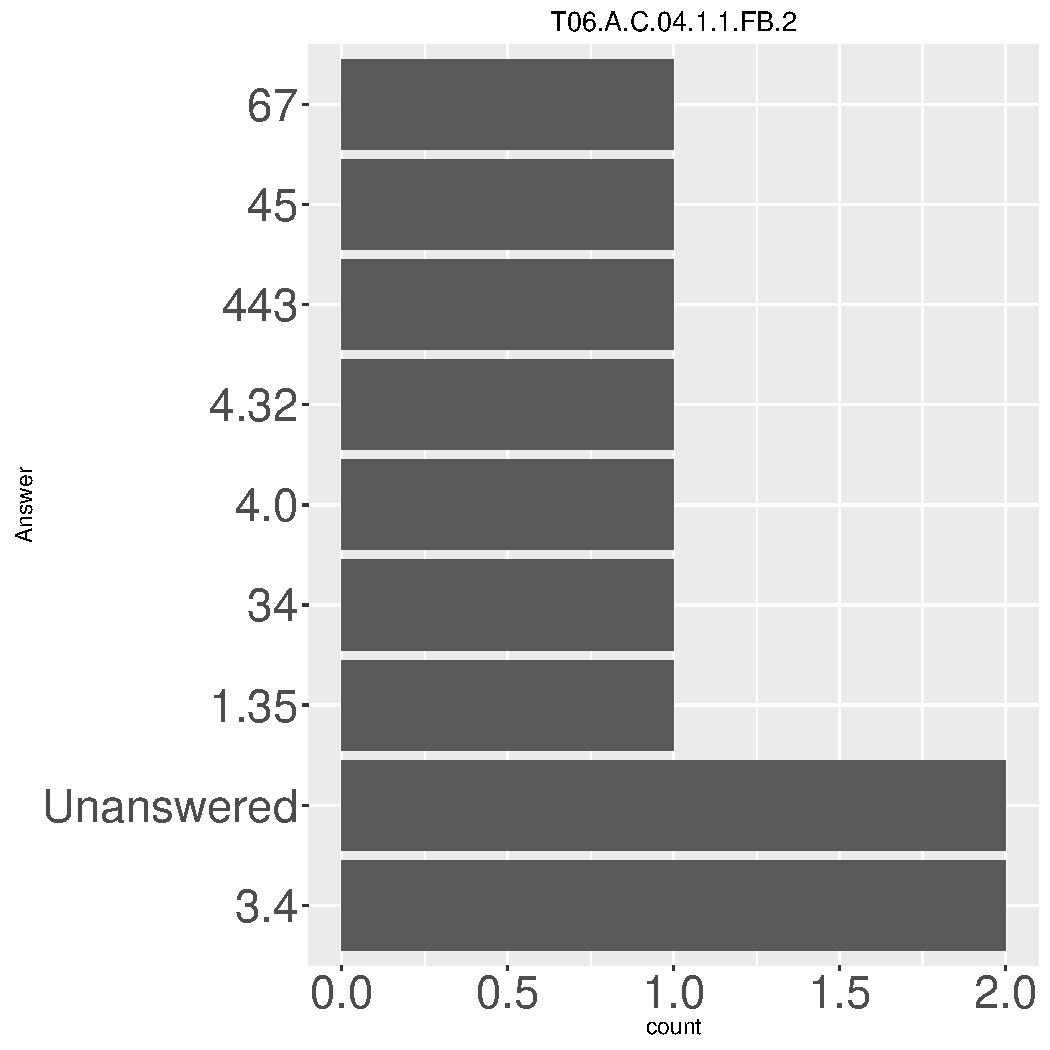
\includegraphics[width=.45\linewidth]{Topic06_AB_10_answer} 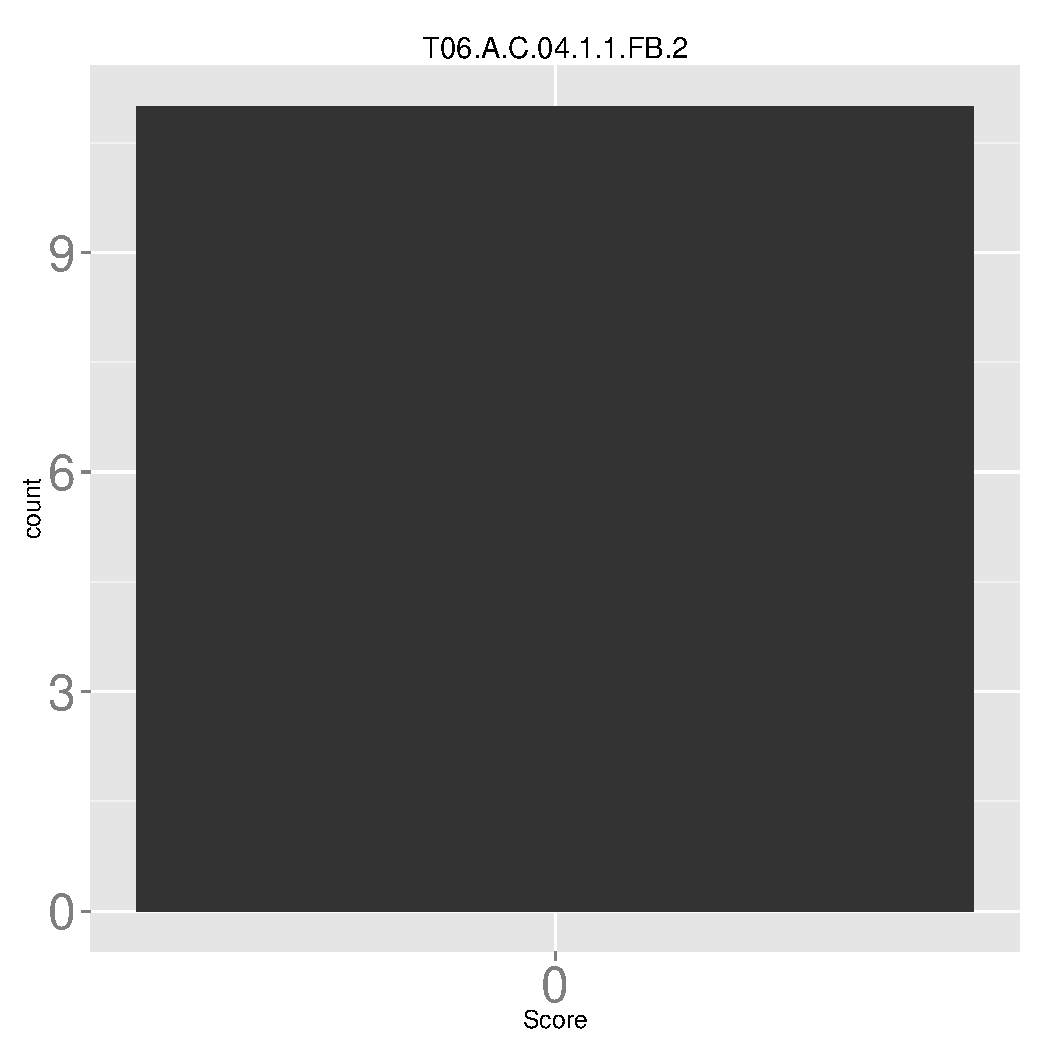
\includegraphics[width=.45\linewidth]{Topic06_AB_10_score} \end{center} 

\begin{center}% latex table generated in R 3.2.2 by xtable 1.8-0 package
% Thu Jan 21 00:33:24 2016
\begin{tabular}{lr}
  \hline
Answer & Count \\ 
  \hline
3.4 &   2 \\ 
  Unanswered &   2 \\ 
  1.35 &   1 \\ 
  34 &   1 \\ 
  4.0 &   1 \\ 
  4.32 &   1 \\ 
  443 &   1 \\ 
  45 &   1 \\ 
  67 &   1 \\ 
   \hline
\end{tabular}
~~~~~~~~% latex table generated in R 3.2.2 by xtable 1.8-0 package
% Thu Jan 21 00:33:24 2016
\begin{tabular}{lr}
  \hline
Summary & Value \\ 
  \hline
Mean & 0.00 \\ 
  Std.dev & 0.00 \\ 
  Min & 0.00 \\ 
  Median & 0.00 \\ 
  Max & 0.00 \\ 
   \hline
\end{tabular}
\end{center}\newpage\marginnote{

 In a sample of 25 male newborns, the mean birth weight was 3.4 kg and the standard deviation was 0.35 kg.



The z-score for a birth weight of 4.2 kg is \_\_\_\_\_\_\_\_\_\_. Round your answer to 2 decimal places.



Correct Answer(s):



a. 2.28



b. 2.29



c. 2.27 

}\pdfbookmark[2]{T06.A.C.04.1.1.FB.3}{T06.A.C.04.1.1.FB.3} (11) Question "T06.A.C.04.1.1.FB.3" is given on the right. This question was selected from the question set with a frequency of 0.25. The question was administered to 14 out of the total of 50 students. The average score was 0 out of 1.

 (Back to the question summary Table \ref{tab:summary_question}.)

\begin{center} 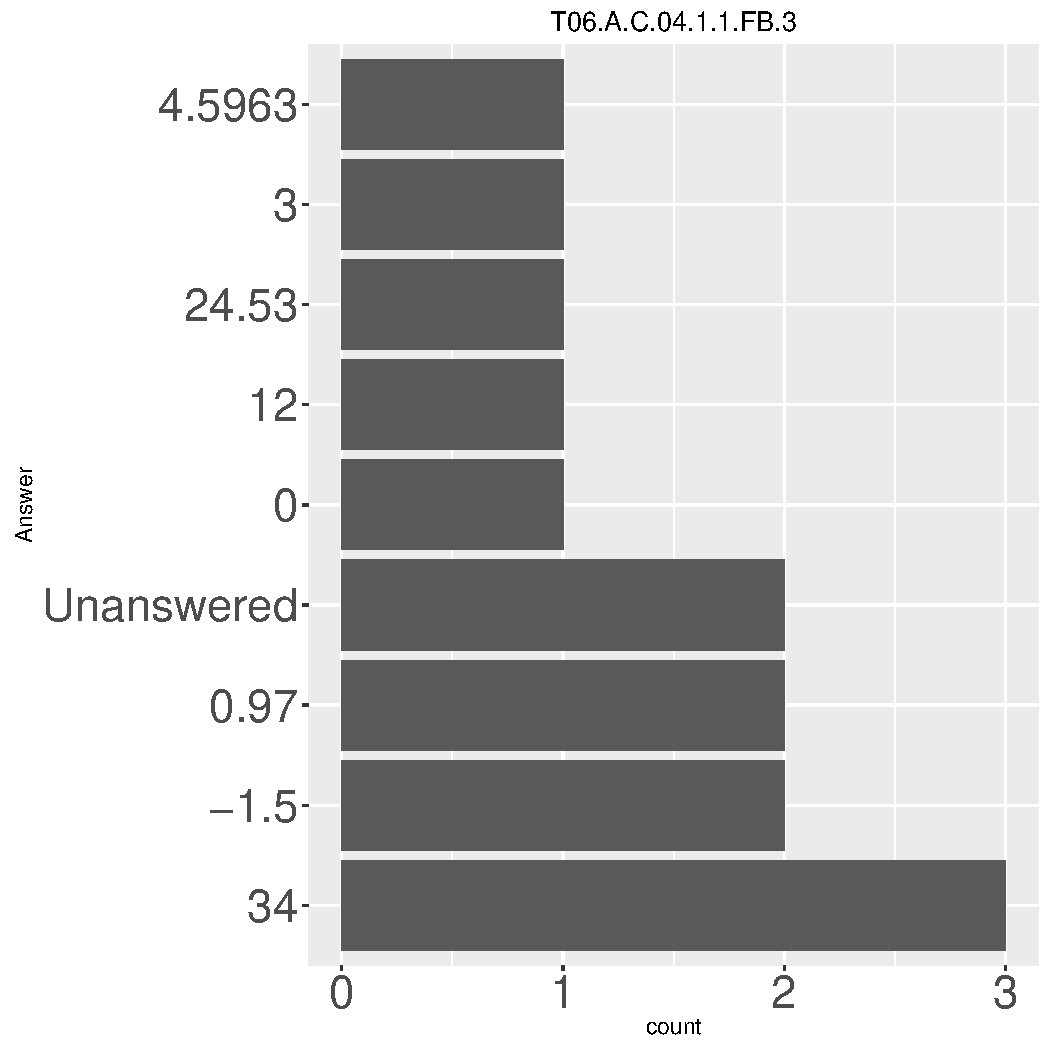
\includegraphics[width=.45\linewidth]{Topic06_AB_11_answer} 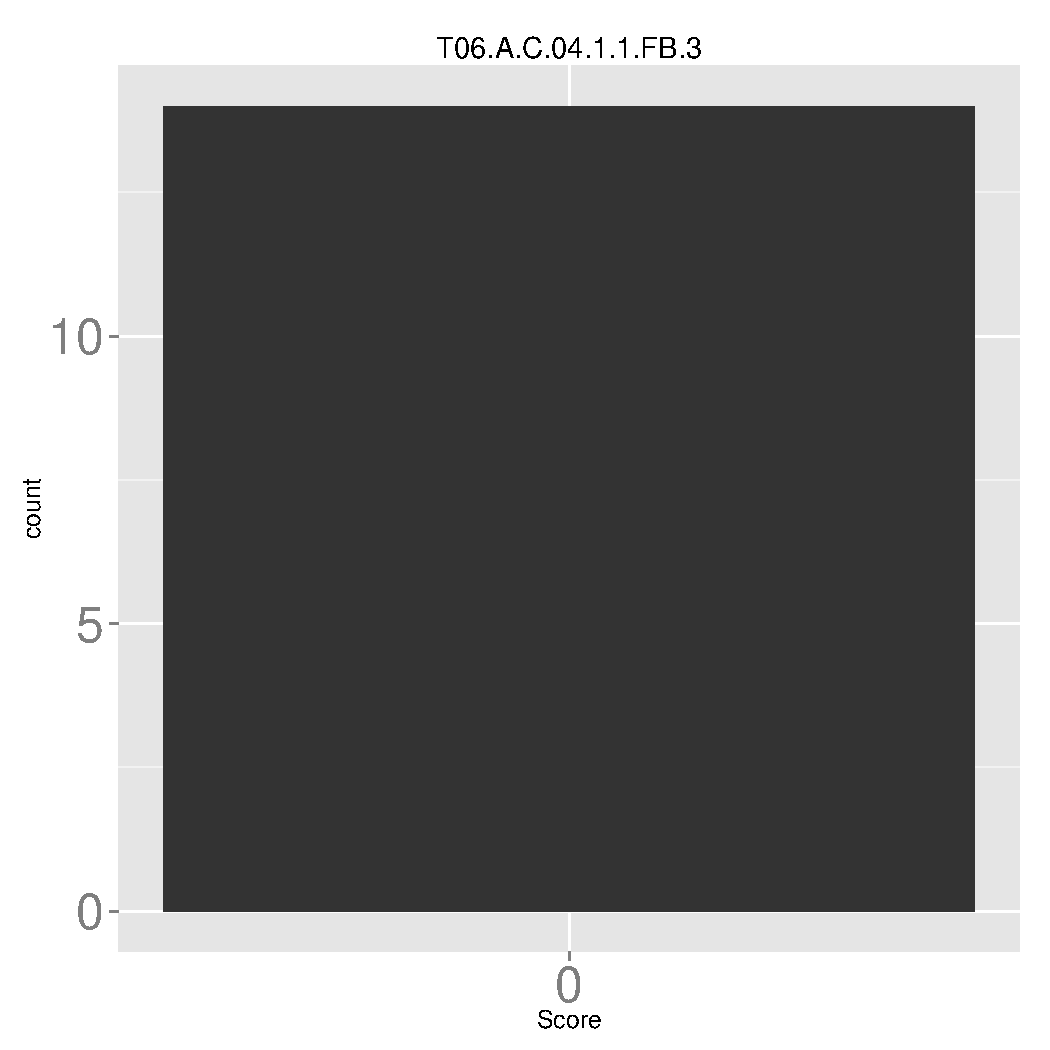
\includegraphics[width=.45\linewidth]{Topic06_AB_11_score} \end{center} 

\begin{center}% latex table generated in R 3.2.2 by xtable 1.8-0 package
% Thu Jan 21 00:33:25 2016
\begin{tabular}{lr}
  \hline
Answer & Count \\ 
  \hline
34 &   3 \\ 
  -1.5 &   2 \\ 
  0.97 &   2 \\ 
  Unanswered &   2 \\ 
  0 &   1 \\ 
  12 &   1 \\ 
  24.53 &   1 \\ 
  3 &   1 \\ 
  4.5963 &   1 \\ 
   \hline
\end{tabular}
~~~~~~~~% latex table generated in R 3.2.2 by xtable 1.8-0 package
% Thu Jan 21 00:33:25 2016
\begin{tabular}{lr}
  \hline
Summary & Value \\ 
  \hline
Mean & 0.00 \\ 
  Std.dev & 0.00 \\ 
  Min & 0.00 \\ 
  Median & 0.00 \\ 
  Max & 0.00 \\ 
   \hline
\end{tabular}
\end{center}\newpage\marginnote{

 In a sample of 25 male newborns, the mean birth weight was 3.4 kg and the standard deviation was 0.35 kg.



The z-score for a birth weight of 4.3 kg is \_\_\_\_\_\_\_\_\_\_. Round your answer to 2 decimal places.



Correct Answer(s):



a. 2.57



b. 2.56



c. 2.58 

}\pdfbookmark[2]{T06.A.C.04.1.1.FB.4}{T06.A.C.04.1.1.FB.4} (12) Question "T06.A.C.04.1.1.FB.4" is given on the right. This question was selected from the question set with a frequency of 0.25. The question was administered to 14 out of the total of 50 students. The average score was 0 out of 1.

 (Back to the question summary Table \ref{tab:summary_question}.)

\begin{center} 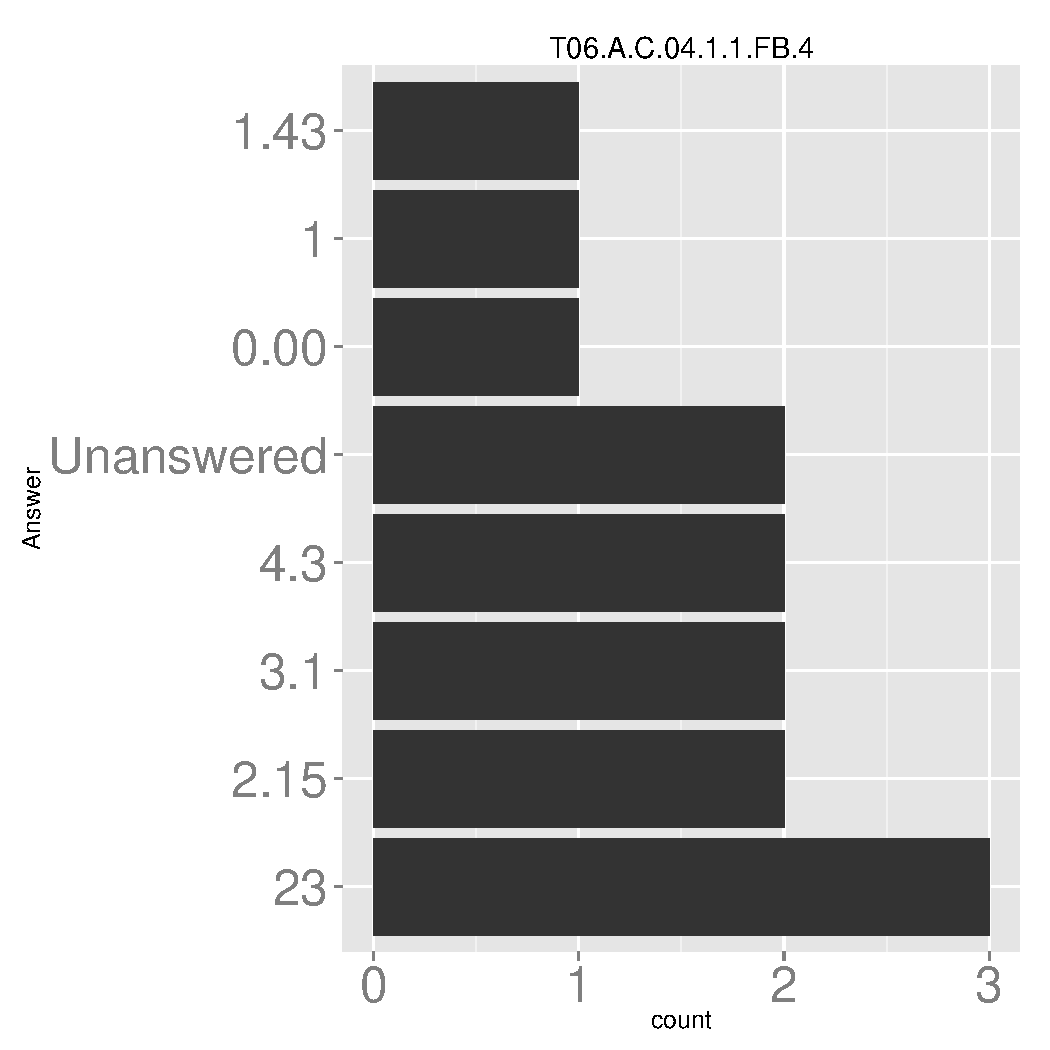
\includegraphics[width=.45\linewidth]{Topic06_AB_12_answer} 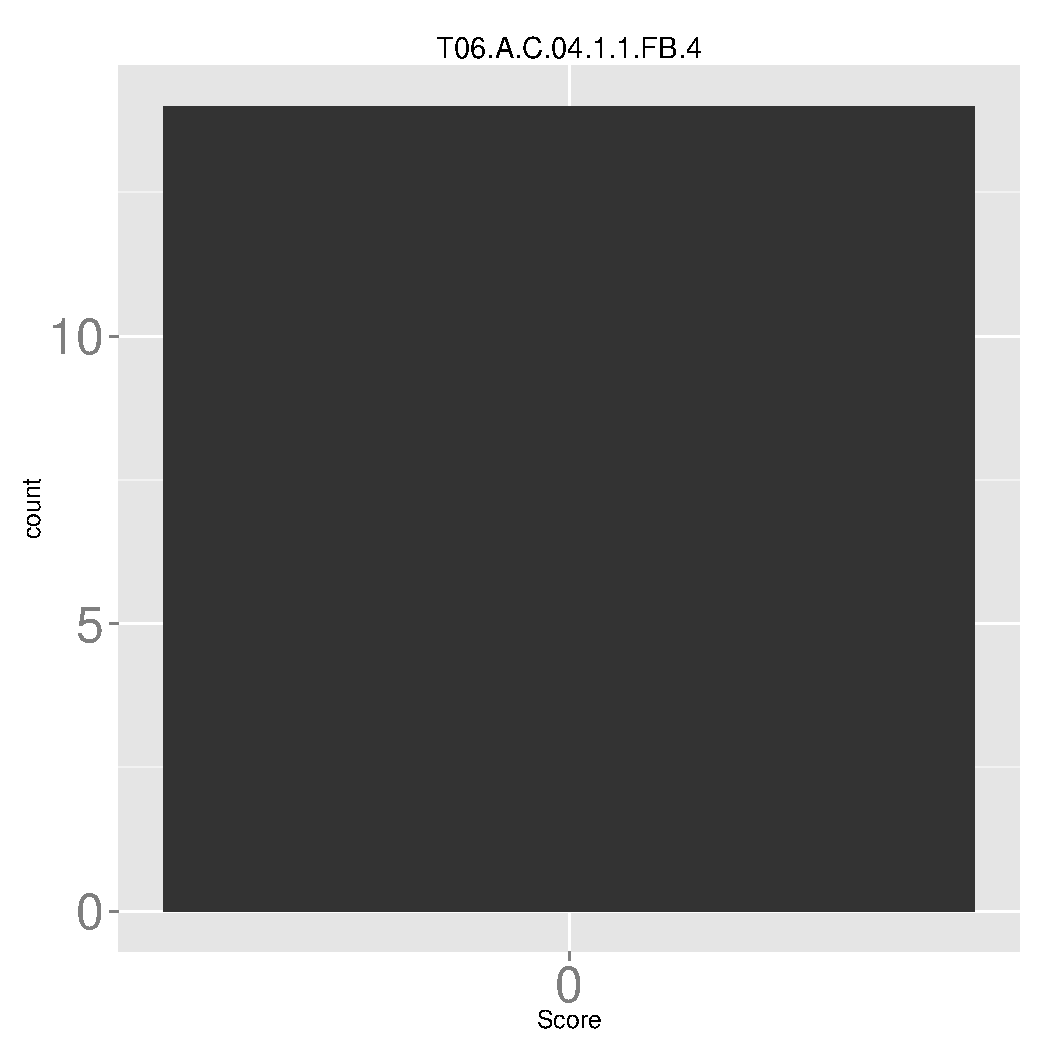
\includegraphics[width=.45\linewidth]{Topic06_AB_12_score} \end{center} 

\begin{center}% latex table generated in R 3.2.2 by xtable 1.8-0 package
% Thu Jan 21 00:33:26 2016
\begin{tabular}{lr}
  \hline
Answer & Count \\ 
  \hline
23 &   3 \\ 
  2.15 &   2 \\ 
  3.1 &   2 \\ 
  4.3 &   2 \\ 
  Unanswered &   2 \\ 
  0.00 &   1 \\ 
  1 &   1 \\ 
  1.43 &   1 \\ 
   \hline
\end{tabular}
~~~~~~~~% latex table generated in R 3.2.2 by xtable 1.8-0 package
% Thu Jan 21 00:33:26 2016
\begin{tabular}{lr}
  \hline
Summary & Value \\ 
  \hline
Mean & 0.00 \\ 
  Std.dev & 0.00 \\ 
  Min & 0.00 \\ 
  Median & 0.00 \\ 
  Max & 0.00 \\ 
   \hline
\end{tabular}
\end{center}\newpage\marginnote{

 In a sample of 25 male newborns, the mean birth weight was 3.4 kg and the standard deviation was 0.35 kg.



The z-score for a birth weight of 2.3 kg is \_\_\_\_\_\_\_\_\_\_. Round your answer to 2 decimal places.



Correct Answer(s):



a. -3.14



b. -3.13



c. -3.15 

}\pdfbookmark[2]{T06.A.D.04.1.1.FB.1}{T06.A.D.04.1.1.FB.1} (13) Question "T06.A.D.04.1.1.FB.1" is given on the right. This question was selected from the question set with a frequency of 0.25. The question was administered to 10 out of the total of 50 students. The average score was 0 out of 1.

 (Back to the question summary Table \ref{tab:summary_question}.)

\begin{center} 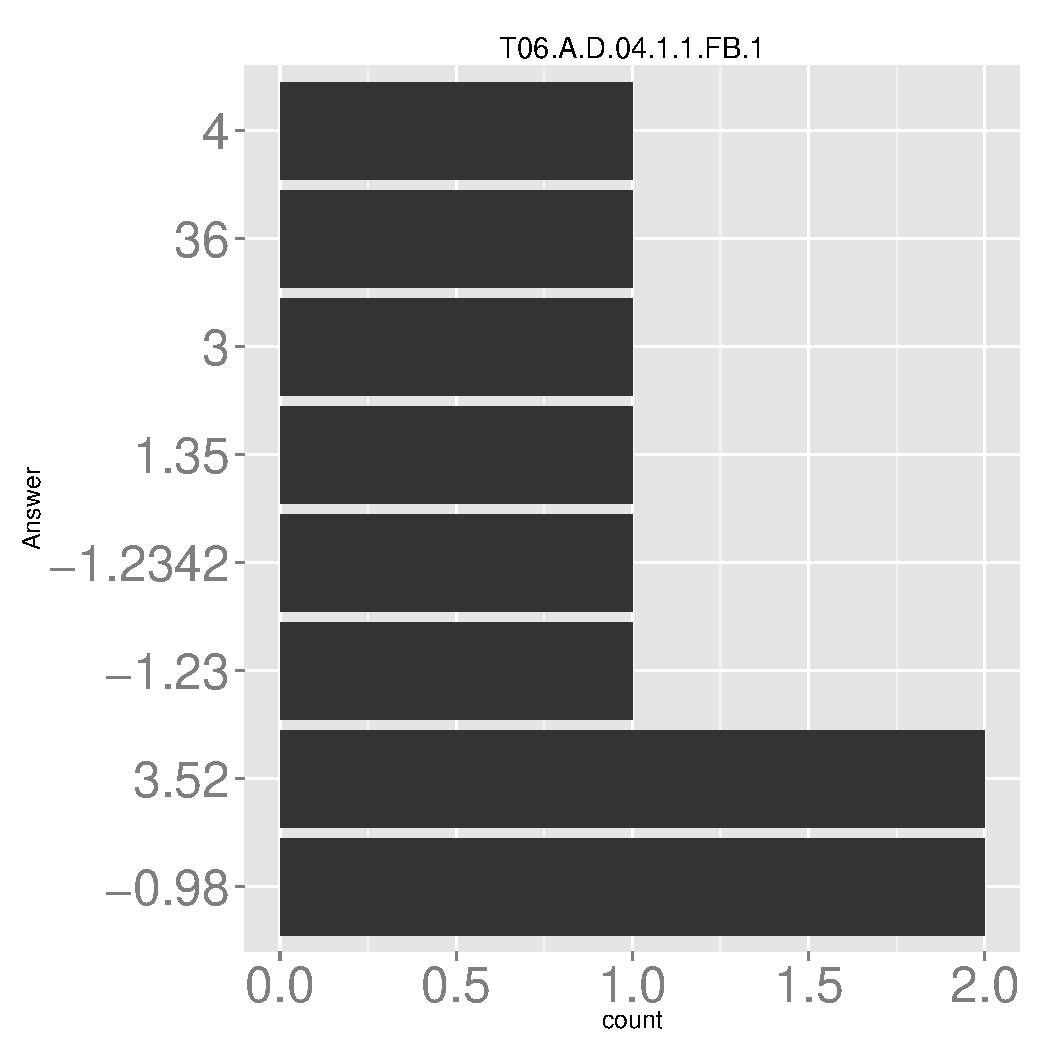
\includegraphics[width=.45\linewidth]{Topic06_AB_13_answer} 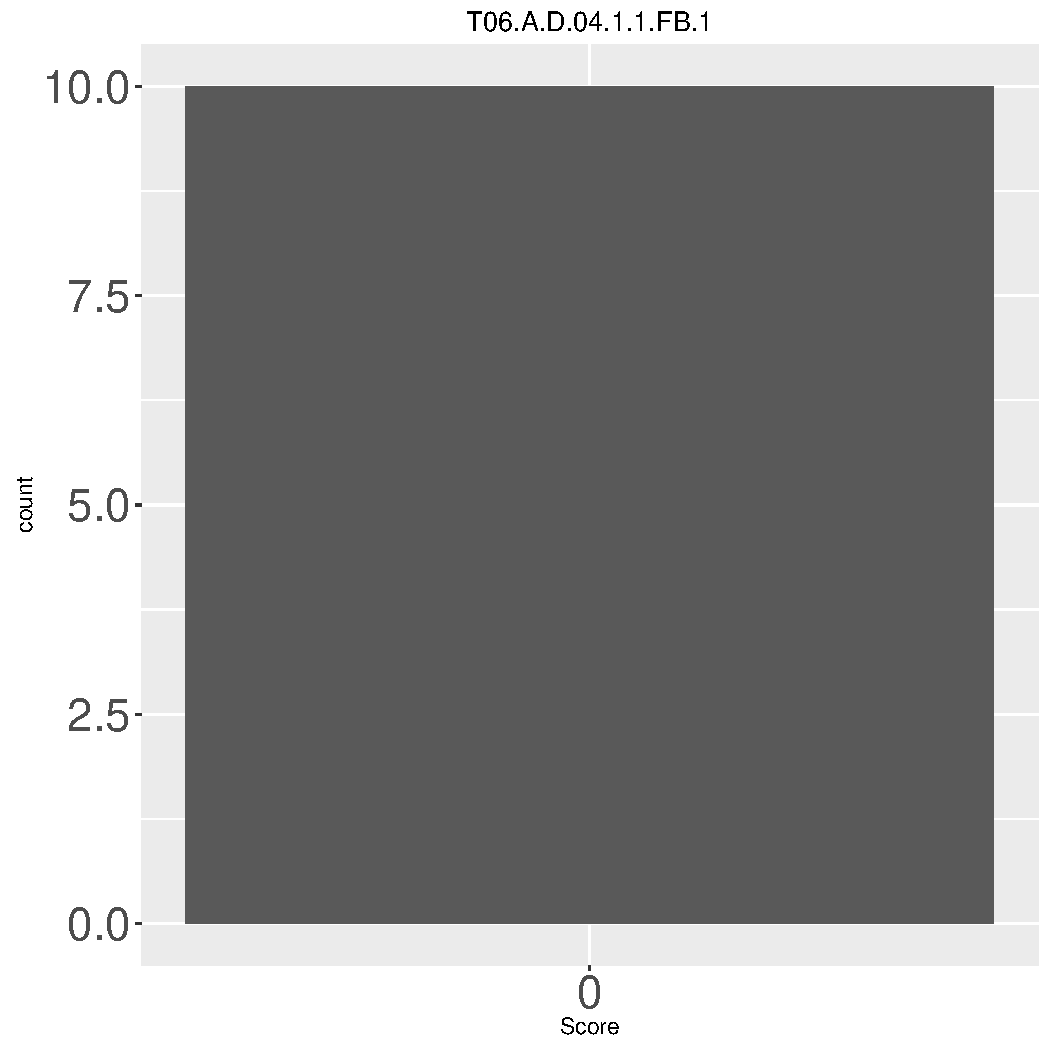
\includegraphics[width=.45\linewidth]{Topic06_AB_13_score} \end{center} 

\begin{center}% latex table generated in R 3.2.2 by xtable 1.8-0 package
% Thu Jan 21 00:33:26 2016
\begin{tabular}{lr}
  \hline
Answer & Count \\ 
  \hline
-0.98 &   2 \\ 
  3.52 &   2 \\ 
  -1.23 &   1 \\ 
  -1.2342 &   1 \\ 
  1.35 &   1 \\ 
  3 &   1 \\ 
  36 &   1 \\ 
  4 &   1 \\ 
   \hline
\end{tabular}
~~~~~~~~% latex table generated in R 3.2.2 by xtable 1.8-0 package
% Thu Jan 21 00:33:26 2016
\begin{tabular}{lr}
  \hline
Summary & Value \\ 
  \hline
Mean & 0.00 \\ 
  Std.dev & 0.00 \\ 
  Min & 0.00 \\ 
  Median & 0.00 \\ 
  Max & 0.00 \\ 
   \hline
\end{tabular}
\end{center}\newpage\marginnote{

 In a sample of 25 male newborns, the mean birth weight was 3.4 kg and the standard deviation was 0.35 kg.



The z-score for a birth weight of 2.5 kg is \_\_\_\_\_\_\_\_\_\_. Round your answer to 2 decimal places.



Correct Answer(s):



a. -2.57



b. -2.58



c. -2.56 

}\pdfbookmark[2]{T06.A.D.04.1.1.FB.2}{T06.A.D.04.1.1.FB.2} (14) Question "T06.A.D.04.1.1.FB.2" is given on the right. This question was selected from the question set with a frequency of 0.25. The question was administered to 13 out of the total of 50 students. The average score was 0 out of 1.

 (Back to the question summary Table \ref{tab:summary_question}.)

\begin{center} 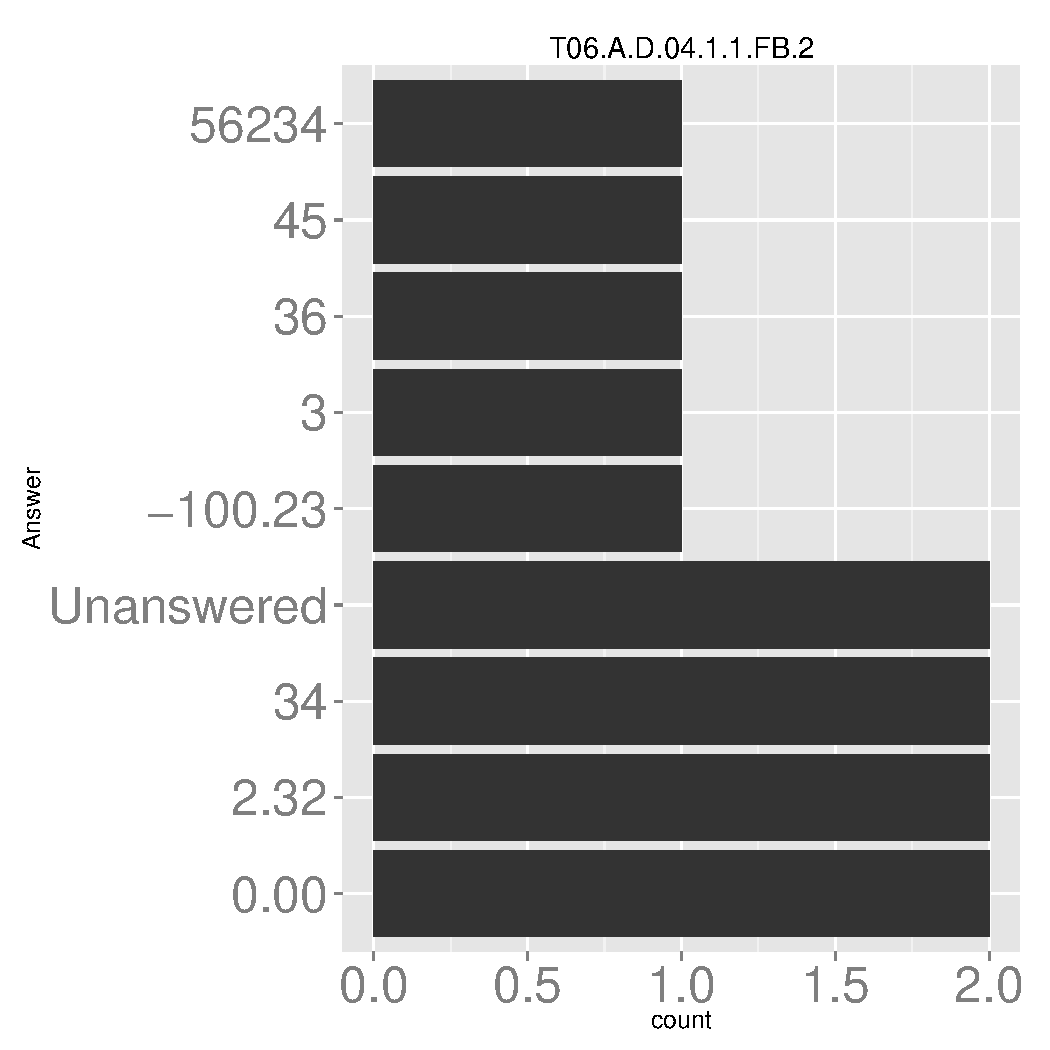
\includegraphics[width=.45\linewidth]{Topic06_AB_14_answer} 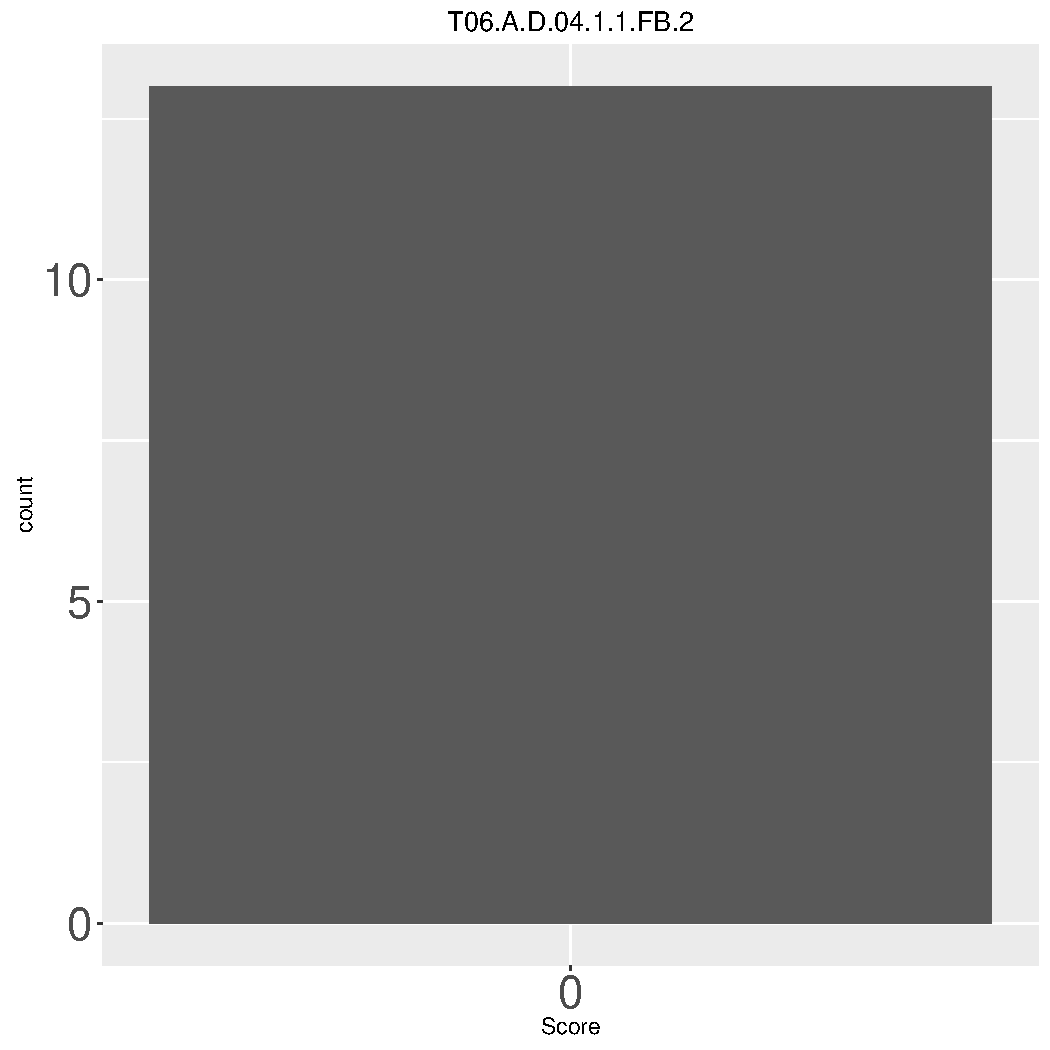
\includegraphics[width=.45\linewidth]{Topic06_AB_14_score} \end{center} 

\begin{center}% latex table generated in R 3.2.2 by xtable 1.8-0 package
% Thu Jan 21 00:33:27 2016
\begin{tabular}{lr}
  \hline
Answer & Count \\ 
  \hline
0.00 &   2 \\ 
  2.32 &   2 \\ 
  34 &   2 \\ 
  Unanswered &   2 \\ 
  -100.23 &   1 \\ 
  3 &   1 \\ 
  36 &   1 \\ 
  45 &   1 \\ 
  56234 &   1 \\ 
   \hline
\end{tabular}
~~~~~~~~% latex table generated in R 3.2.2 by xtable 1.8-0 package
% Thu Jan 21 00:33:27 2016
\begin{tabular}{lr}
  \hline
Summary & Value \\ 
  \hline
Mean & 0.00 \\ 
  Std.dev & 0.00 \\ 
  Min & 0.00 \\ 
  Median & 0.00 \\ 
  Max & 0.00 \\ 
   \hline
\end{tabular}
\end{center}\newpage\marginnote{

 In a sample of 25 male newborns, the mean birth weight was 3.4 kg and the standard deviation was 0.35 kg.



The z-score for a birth weight of 2.2 kg is \_\_\_\_\_\_\_\_\_\_. Round your answer to 2 decimal places.



Correct Answer(s):



a. -3.43



b. -3.44



c. -3.42 

}\pdfbookmark[2]{T06.A.D.04.1.1.FB.3}{T06.A.D.04.1.1.FB.3} (15) Question "T06.A.D.04.1.1.FB.3" is given on the right. This question was selected from the question set with a frequency of 0.25. The question was administered to 11 out of the total of 50 students. The average score was 0 out of 1.

 (Back to the question summary Table \ref{tab:summary_question}.)

\begin{center} 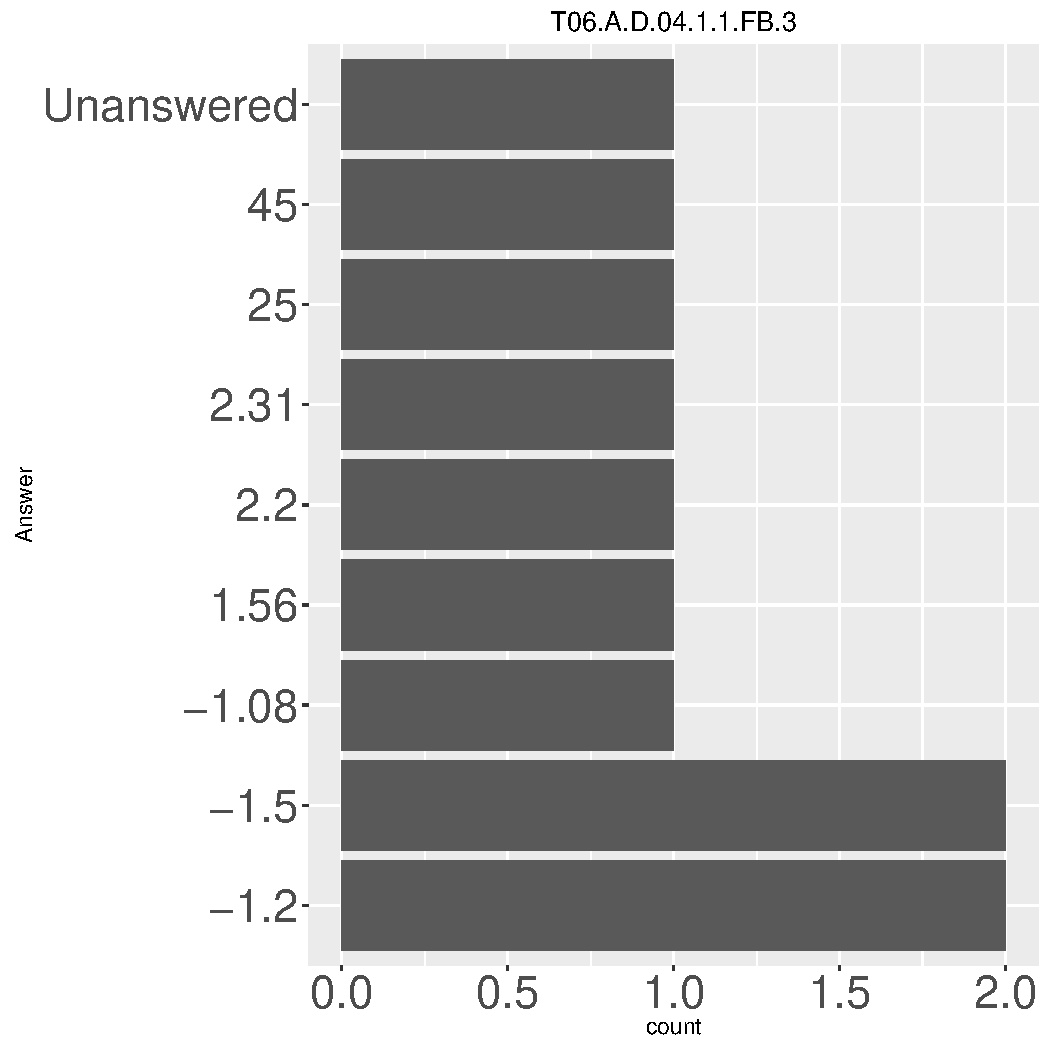
\includegraphics[width=.45\linewidth]{Topic06_AB_15_answer} 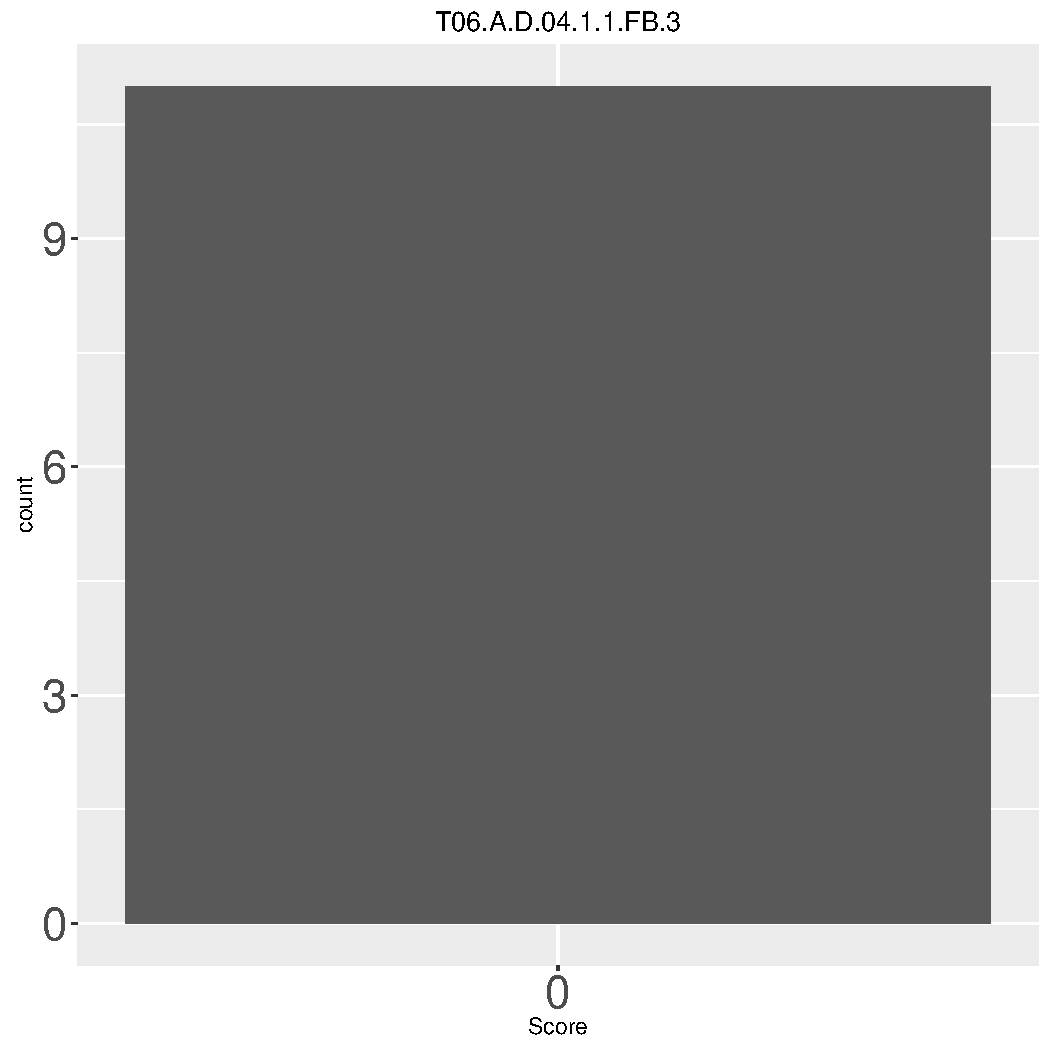
\includegraphics[width=.45\linewidth]{Topic06_AB_15_score} \end{center} 

\begin{center}% latex table generated in R 3.2.2 by xtable 1.8-0 package
% Thu Jan 21 00:33:28 2016
\begin{tabular}{lr}
  \hline
Answer & Count \\ 
  \hline
-1.2 &   2 \\ 
  -1.5 &   2 \\ 
  -1.08 &   1 \\ 
  1.56 &   1 \\ 
  2.2 &   1 \\ 
  2.31 &   1 \\ 
  25 &   1 \\ 
  45 &   1 \\ 
  Unanswered &   1 \\ 
   \hline
\end{tabular}
~~~~~~~~% latex table generated in R 3.2.2 by xtable 1.8-0 package
% Thu Jan 21 00:33:28 2016
\begin{tabular}{lr}
  \hline
Summary & Value \\ 
  \hline
Mean & 0.00 \\ 
  Std.dev & 0.00 \\ 
  Min & 0.00 \\ 
  Median & 0.00 \\ 
  Max & 0.00 \\ 
   \hline
\end{tabular}
\end{center}\newpage\marginnote{

 In a sample of 25 male newborns, the mean birth weight was 3.4 kg and the standard deviation was 0.35 kg.



The z-score for a birth weight of 2.8 kg is \_\_\_\_\_\_\_\_\_\_. Round your answer to 2 decimal places.



Correct Answer(s):



a. -1.71



b. -1.72



c. -1.70



d. -1.7 

}\pdfbookmark[2]{T06.A.D.04.1.1.FB.4}{T06.A.D.04.1.1.FB.4} (16) Question "T06.A.D.04.1.1.FB.4" is given on the right. This question was selected from the question set with a frequency of 0.25. The question was administered to 16 out of the total of 50 students. The average score was 0 out of 1.

 (Back to the question summary Table \ref{tab:summary_question}.)

\begin{center} 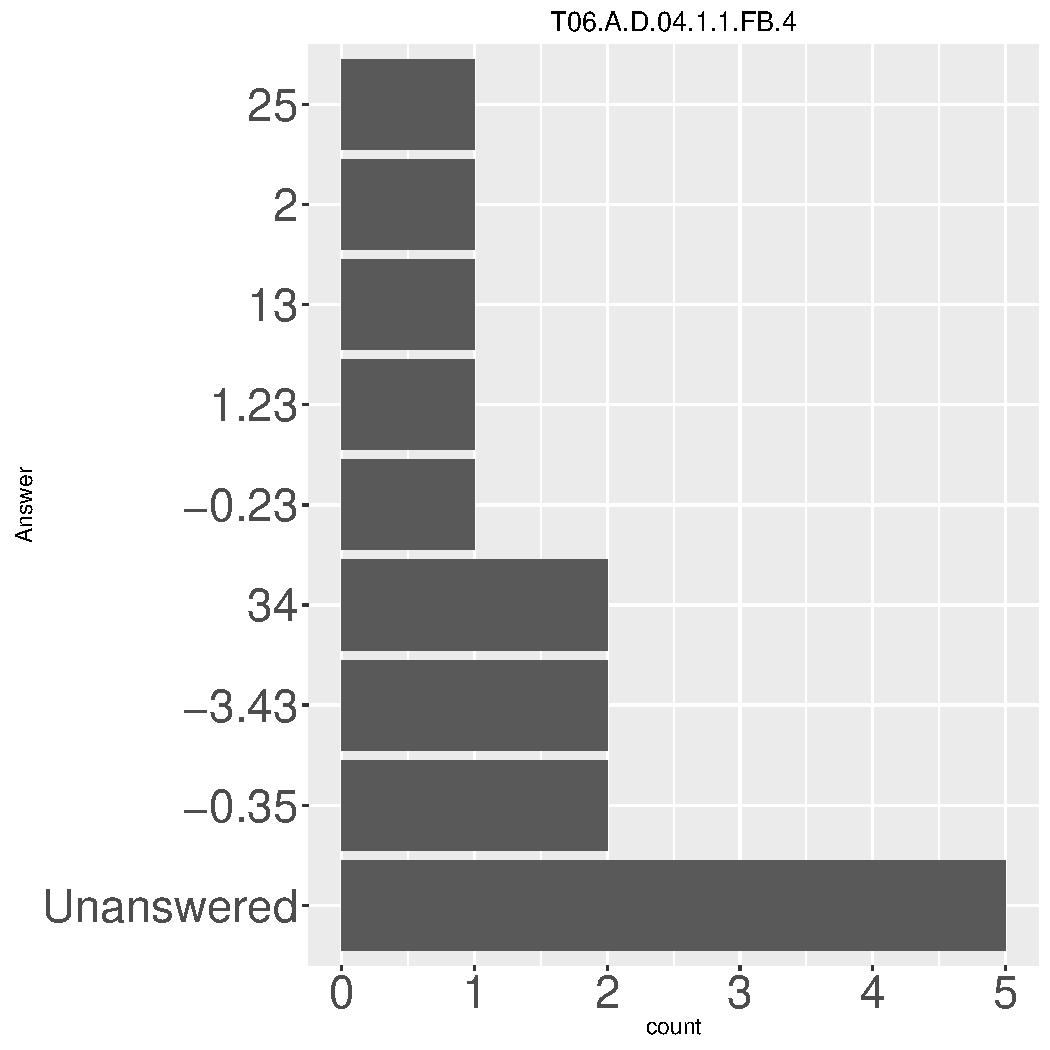
\includegraphics[width=.45\linewidth]{Topic06_AB_16_answer} 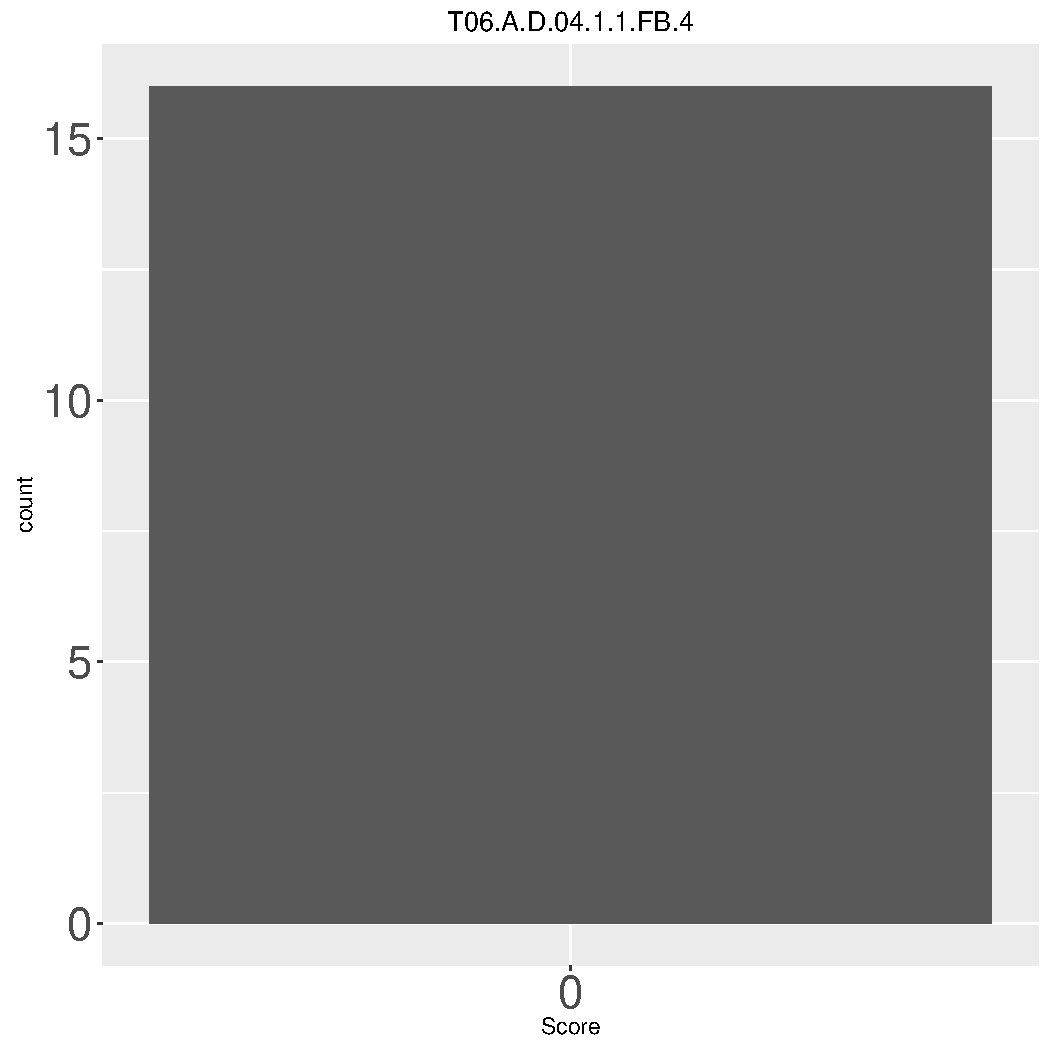
\includegraphics[width=.45\linewidth]{Topic06_AB_16_score} \end{center} 

\begin{center}% latex table generated in R 3.2.2 by xtable 1.8-0 package
% Thu Jan 21 00:33:29 2016
\begin{tabular}{lr}
  \hline
Answer & Count \\ 
  \hline
Unanswered &   5 \\ 
  -0.35 &   2 \\ 
  -3.43 &   2 \\ 
  34 &   2 \\ 
  -0.23 &   1 \\ 
  1.23 &   1 \\ 
  13 &   1 \\ 
  2 &   1 \\ 
  25 &   1 \\ 
   \hline
\end{tabular}
~~~~~~~~% latex table generated in R 3.2.2 by xtable 1.8-0 package
% Thu Jan 21 00:33:29 2016
\begin{tabular}{lr}
  \hline
Summary & Value \\ 
  \hline
Mean & 0.00 \\ 
  Std.dev & 0.00 \\ 
  Min & 0.00 \\ 
  Median & 0.00 \\ 
  Max & 0.00 \\ 
   \hline
\end{tabular}
\end{center}\newpage\marginnote{

 The height of adult women is thought to have a mean of 65 inches and a standard deviation of 2.5 inches. The height of adult men is thought to have a mean of 71 inches and a standard deviation of 3 inches. In the same family, the son is 73 inches tall and the daughter is 67 inches tall. Who is taller among their gender, the son or daughter?



*a. The daughter



b. The son



c. The daughter and son are the same height within their gender. 

}\pdfbookmark[2]{T06.B.E.01.1.1.MC.compare1}{T06.B.E.01.1.1.MC.compare1} (17) Question "T06.B.E.01.1.1.MC.compare1" is given on the right. This question was selected from the question set with a frequency of 1. The question was administered to 50 out of the total of 50 students. The average score was 0.4 out of 1.

 (Back to the question summary Table \ref{tab:summary_question}.)

\begin{center} 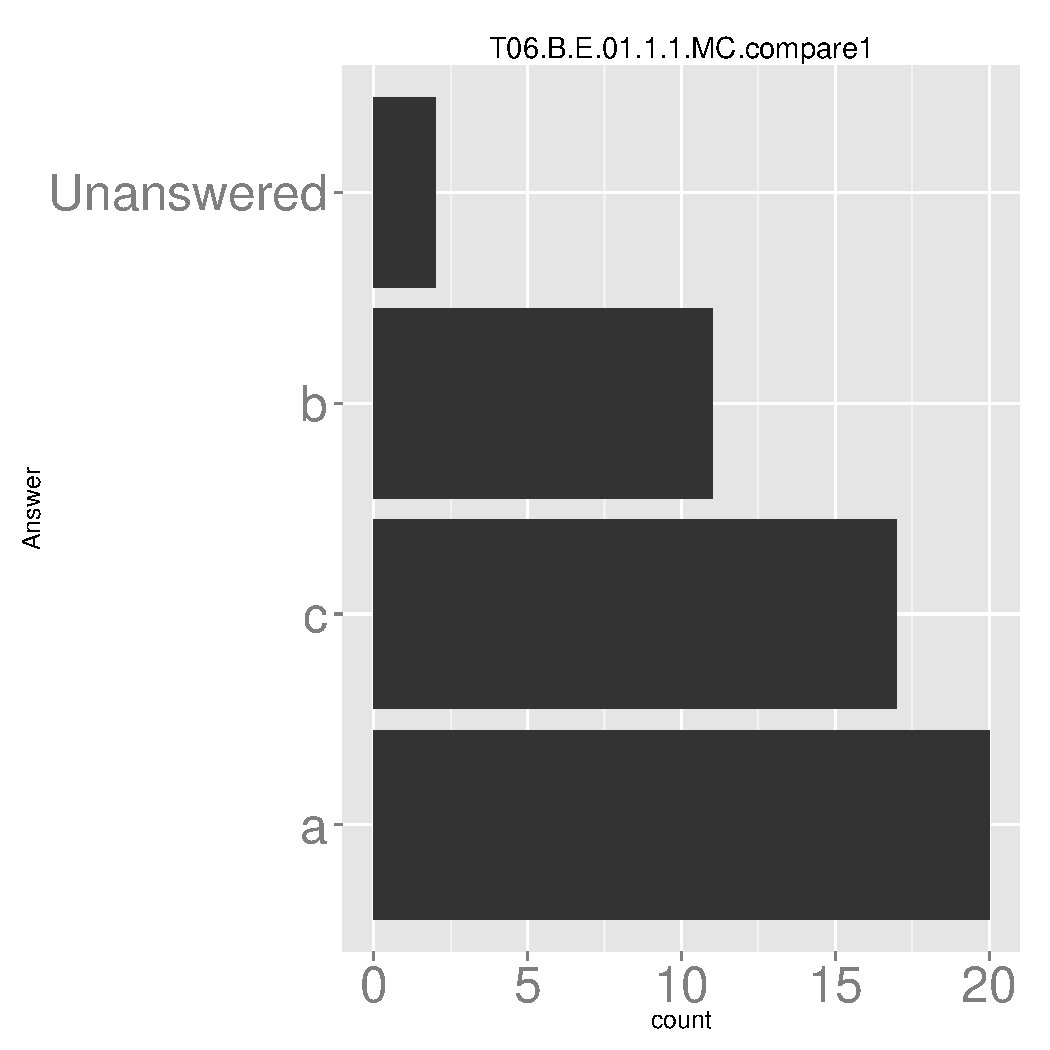
\includegraphics[width=.45\linewidth]{Topic06_AB_17_answer} 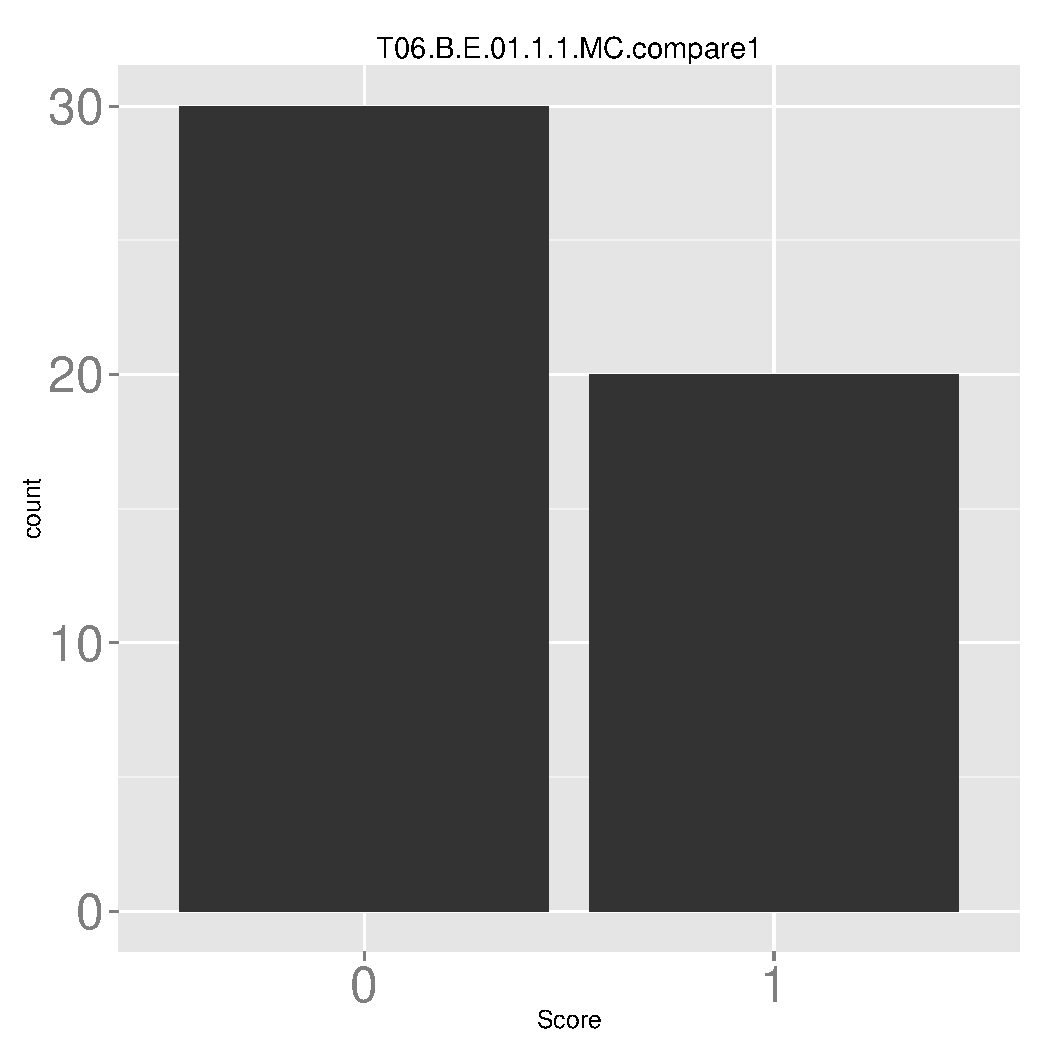
\includegraphics[width=.45\linewidth]{Topic06_AB_17_score} \end{center} 

\begin{center}% latex table generated in R 3.2.2 by xtable 1.8-0 package
% Thu Jan 21 00:33:30 2016
\begin{tabular}{lr}
  \hline
Answer & Count \\ 
  \hline
a &  20 \\ 
  c &  17 \\ 
  b &  11 \\ 
  Unanswered &   2 \\ 
   \hline
\end{tabular}
~~~~~~~~% latex table generated in R 3.2.2 by xtable 1.8-0 package
% Thu Jan 21 00:33:30 2016
\begin{tabular}{lr}
  \hline
Summary & Value \\ 
  \hline
Mean & 0.40 \\ 
  Std.dev & 0.49 \\ 
  Min & 0.00 \\ 
  Median & 0.00 \\ 
  Max & 1.00 \\ 
   \hline
\end{tabular}
\end{center}\newpage\marginnote{

 The height of adult women is thought to have a mean of 65 inches and a standard deviation of 2.5 inches. The height of adult men is thought to have a mean of 71 inches and a standard deviation of 3 inches. In the same family, the son is 67 inches tall and the daughter is 59 inches tall. Who is taller among their gender, the son or daughter?



a. The daughter



*b. The son



c. The daughter and son are the same height within their gender. 

}\pdfbookmark[2]{T06.B.F.01.1.1.MC.compare2}{T06.B.F.01.1.1.MC.compare2} (18) Question "T06.B.F.01.1.1.MC.compare2" is given on the right. This question was selected from the question set with a frequency of 1. The question was administered to 50 out of the total of 50 students. The average score was 0.36 out of 1.

 (Back to the question summary Table \ref{tab:summary_question}.)

\begin{center} 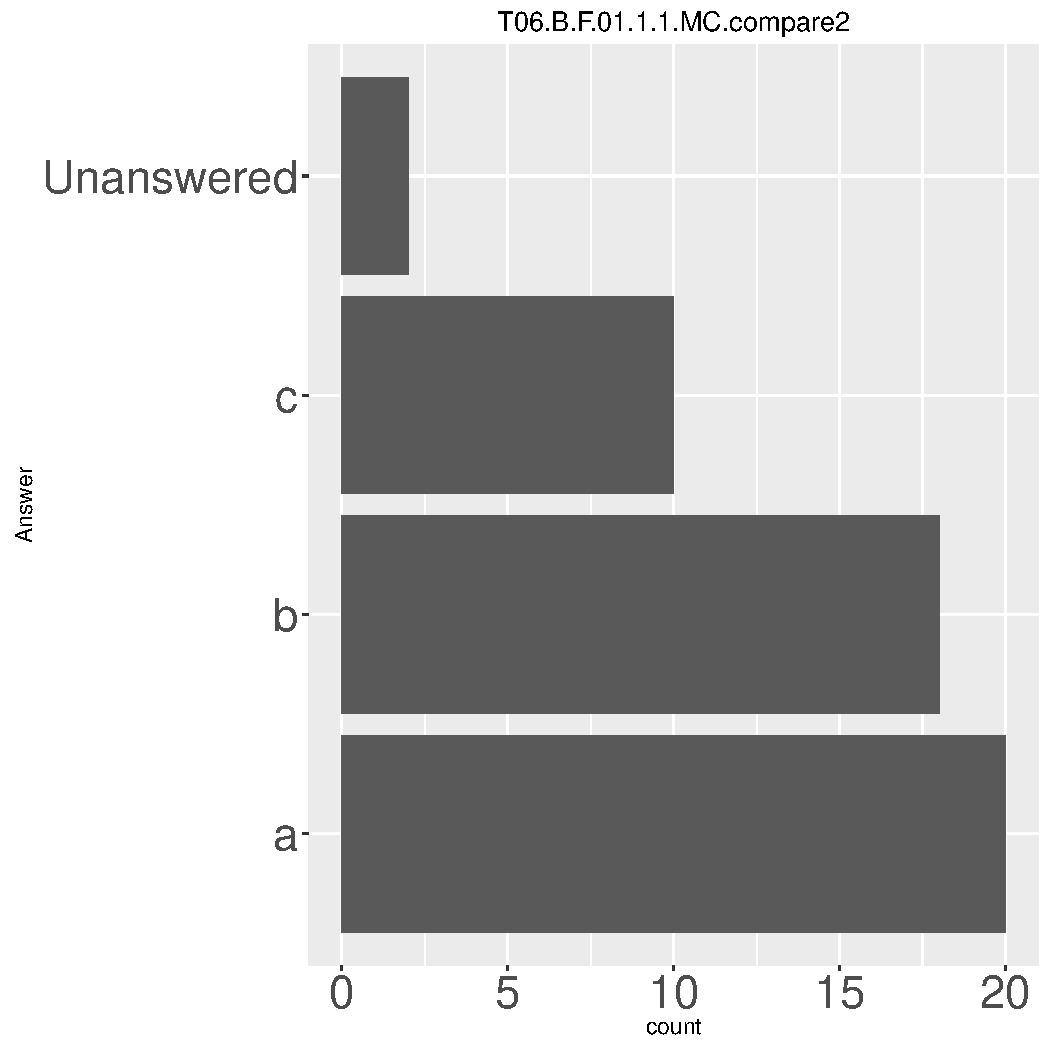
\includegraphics[width=.45\linewidth]{Topic06_AB_18_answer} 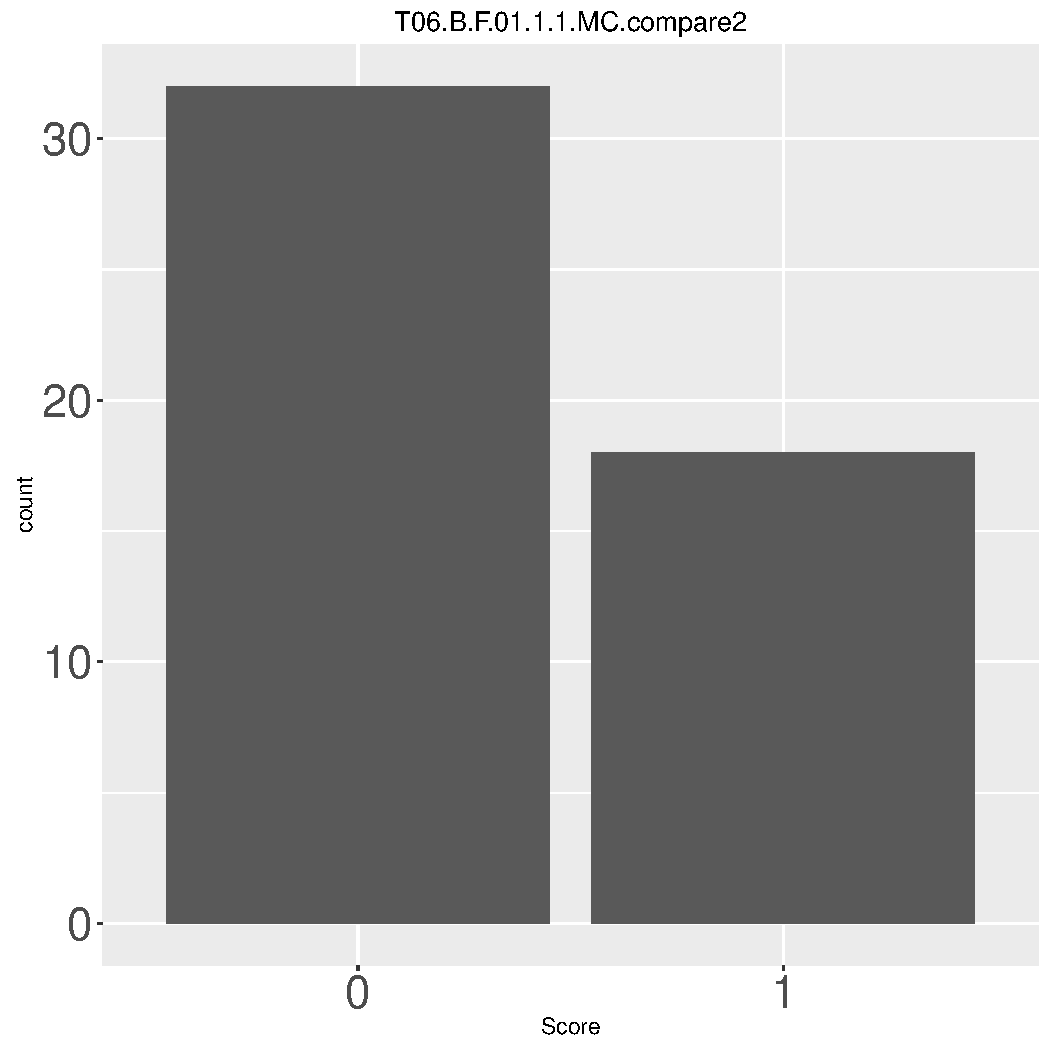
\includegraphics[width=.45\linewidth]{Topic06_AB_18_score} \end{center} 

\begin{center}% latex table generated in R 3.2.2 by xtable 1.8-0 package
% Thu Jan 21 00:33:31 2016
\begin{tabular}{lr}
  \hline
Answer & Count \\ 
  \hline
a &  20 \\ 
  b &  18 \\ 
  c &  10 \\ 
  Unanswered &   2 \\ 
   \hline
\end{tabular}
~~~~~~~~% latex table generated in R 3.2.2 by xtable 1.8-0 package
% Thu Jan 21 00:33:31 2016
\begin{tabular}{lr}
  \hline
Summary & Value \\ 
  \hline
Mean & 0.36 \\ 
  Std.dev & 0.48 \\ 
  Min & 0.00 \\ 
  Median & 0.00 \\ 
  Max & 1.00 \\ 
   \hline
\end{tabular}
\end{center}\newpage\marginnote{

 Standardizing makes the following change(s) to a distribution: I. Shifts the distribution by subtracting the mean. II. Rescales the distribution by dividing by the standard deviation. III. Changes the skewness or symmetry of the distribution. IV. Creates outliers.



a. I, II, and III



*b. I and II



c. III and IV



d. II and III



e. I, II and IV 

}\pdfbookmark[2]{T06.C.G.01.1.1.MC.1}{T06.C.G.01.1.1.MC.1} (19) Question "T06.C.G.01.1.1.MC.1" is given on the right. This question was selected from the question set with a frequency of 1. The question was administered to 50 out of the total of 50 students. The average score was 0.2 out of 1.

 (Back to the question summary Table \ref{tab:summary_question}.)

\begin{center} 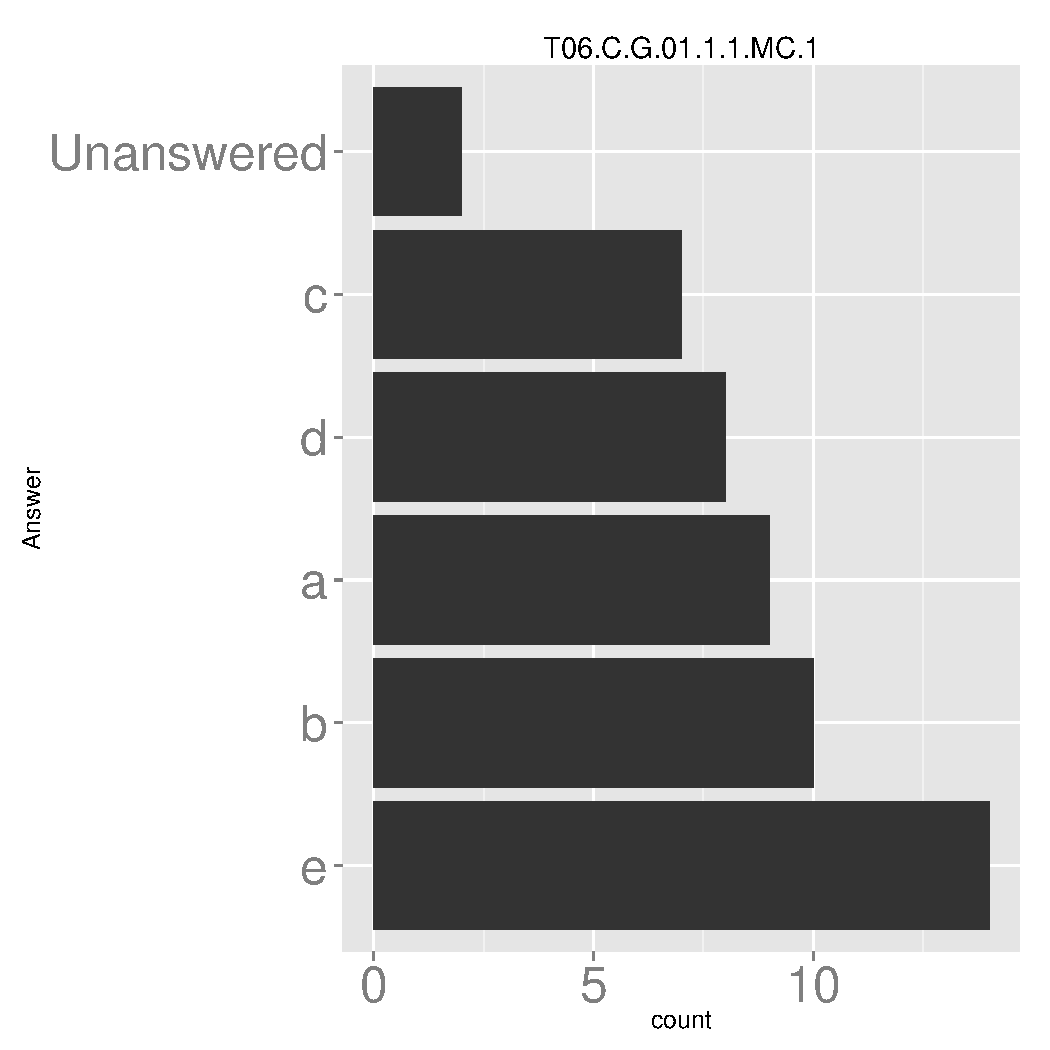
\includegraphics[width=.45\linewidth]{Topic06_AB_19_answer} 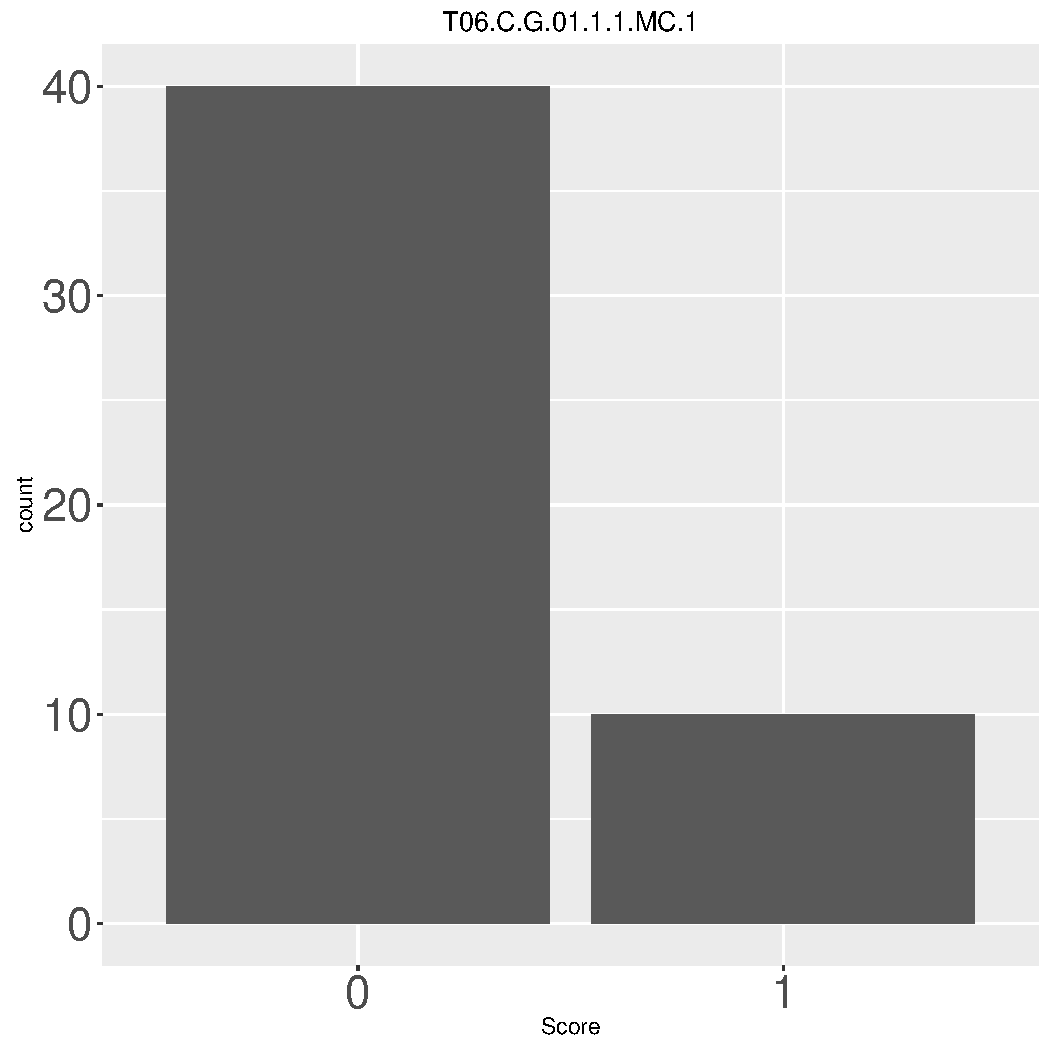
\includegraphics[width=.45\linewidth]{Topic06_AB_19_score} \end{center} 

\begin{center}% latex table generated in R 3.2.2 by xtable 1.8-0 package
% Thu Jan 21 00:33:32 2016
\begin{tabular}{lr}
  \hline
Answer & Count \\ 
  \hline
e &  14 \\ 
  b &  10 \\ 
  a &   9 \\ 
  d &   8 \\ 
  c &   7 \\ 
  Unanswered &   2 \\ 
   \hline
\end{tabular}
~~~~~~~~% latex table generated in R 3.2.2 by xtable 1.8-0 package
% Thu Jan 21 00:33:32 2016
\begin{tabular}{lr}
  \hline
Summary & Value \\ 
  \hline
Mean & 0.20 \\ 
  Std.dev & 0.40 \\ 
  Min & 0.00 \\ 
  Median & 0.00 \\ 
  Max & 1.00 \\ 
   \hline
\end{tabular}
\end{center}\newpage\marginnote{

 Which part of the distribution is NOT affected by standardizing?



*a. shape



b. median



c. IQR



d. range 

}\pdfbookmark[2]{T06.C.H.01.1.1.MC.1}{T06.C.H.01.1.1.MC.1} (20) Question "T06.C.H.01.1.1.MC.1" is given on the right. This question was selected from the question set with a frequency of 1. The question was administered to 50 out of the total of 50 students. The average score was 0.24 out of 1.

 (Back to the question summary Table \ref{tab:summary_question}.)

\begin{center} 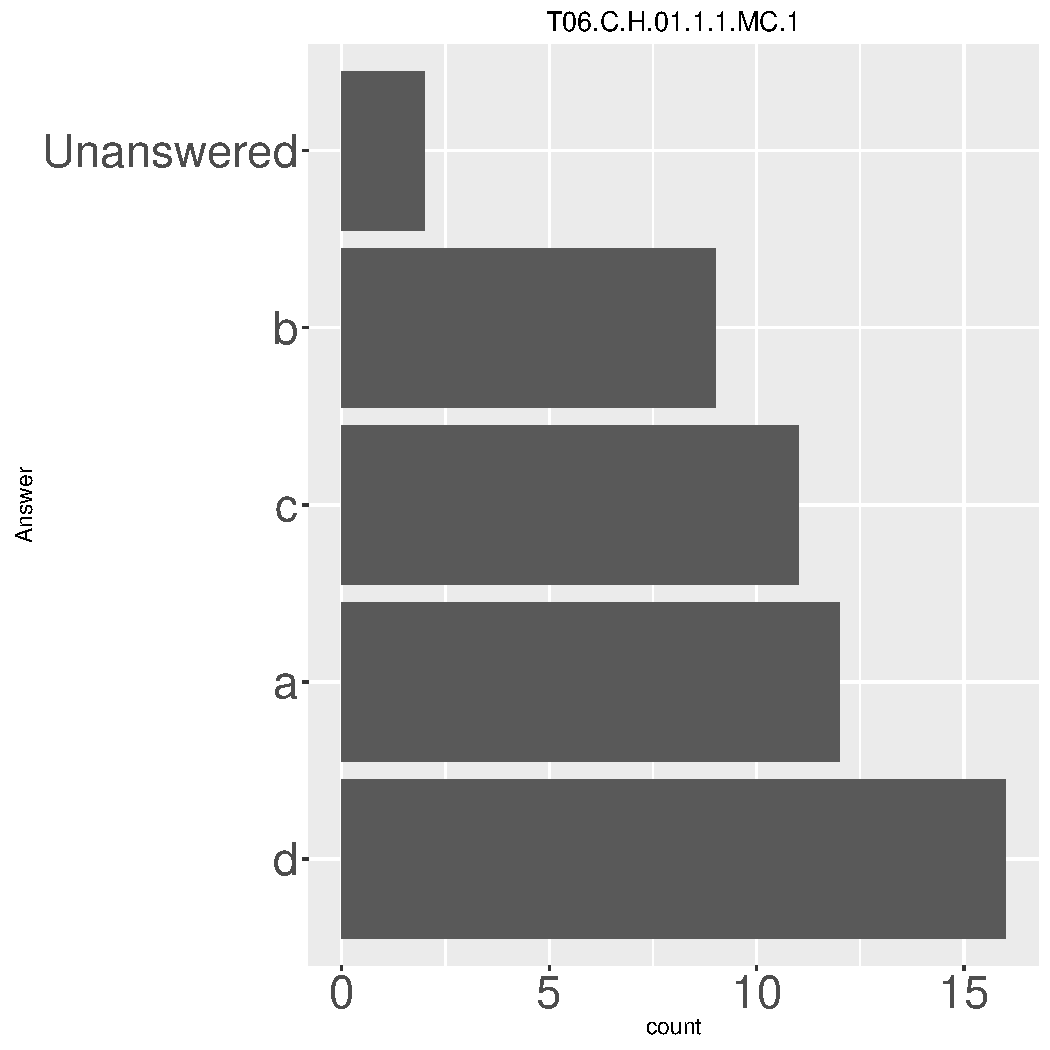
\includegraphics[width=.45\linewidth]{Topic06_AB_20_answer} 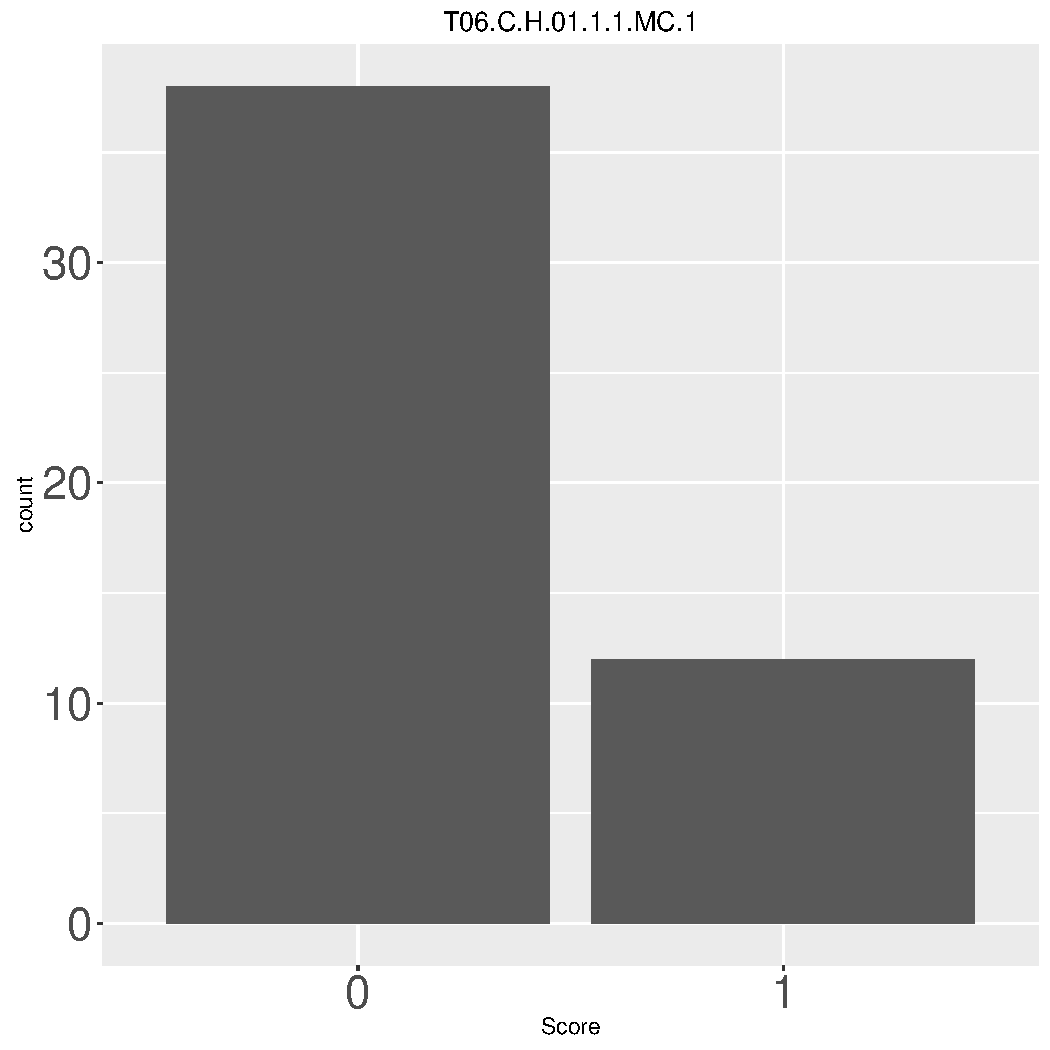
\includegraphics[width=.45\linewidth]{Topic06_AB_20_score} \end{center} 

\begin{center}% latex table generated in R 3.2.2 by xtable 1.8-0 package
% Thu Jan 21 00:33:33 2016
\begin{tabular}{lr}
  \hline
Answer & Count \\ 
  \hline
d &  16 \\ 
  a &  12 \\ 
  c &  11 \\ 
  b &   9 \\ 
  Unanswered &   2 \\ 
   \hline
\end{tabular}
~~~~~~~~% latex table generated in R 3.2.2 by xtable 1.8-0 package
% Thu Jan 21 00:33:33 2016
\begin{tabular}{lr}
  \hline
Summary & Value \\ 
  \hline
Mean & 0.24 \\ 
  Std.dev & 0.43 \\ 
  Min & 0.00 \\ 
  Median & 0.00 \\ 
  Max & 1.00 \\ 
   \hline
\end{tabular}
\end{center}\newpage\marginnote{

 NBA players tend to have very large feet. The following plots display what these shoe sizes may hypothetically look like. Based on the output, it is reasonable to model the distribution of NBA players shoe sizes with a normal distribution. 

}



\vspace{5cm}\begin{marginfigure}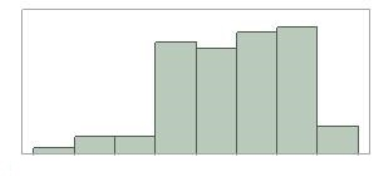
\includegraphics[width=0.98\linewidth]{/Users/lindz/ePort/inst/extdata/KeyFiles/Topic06.Questions_files/image002}\end{marginfigure}\marginnote{

 *a. True



b. False 

}\vspace{-5cm}\pdfbookmark[2]{T06.D.I.02.1.1.TF.feet}{T06.D.I.02.1.1.TF.feet} (21) Question "T06.D.I.02.1.1.TF.feet" is given on the right. This question was selected from the question set with a frequency of 0.5. The question was administered to 20 out of the total of 50 students. The average score was 0.65 out of 1.

 (Back to the question summary Table \ref{tab:summary_question}.)

\begin{center} 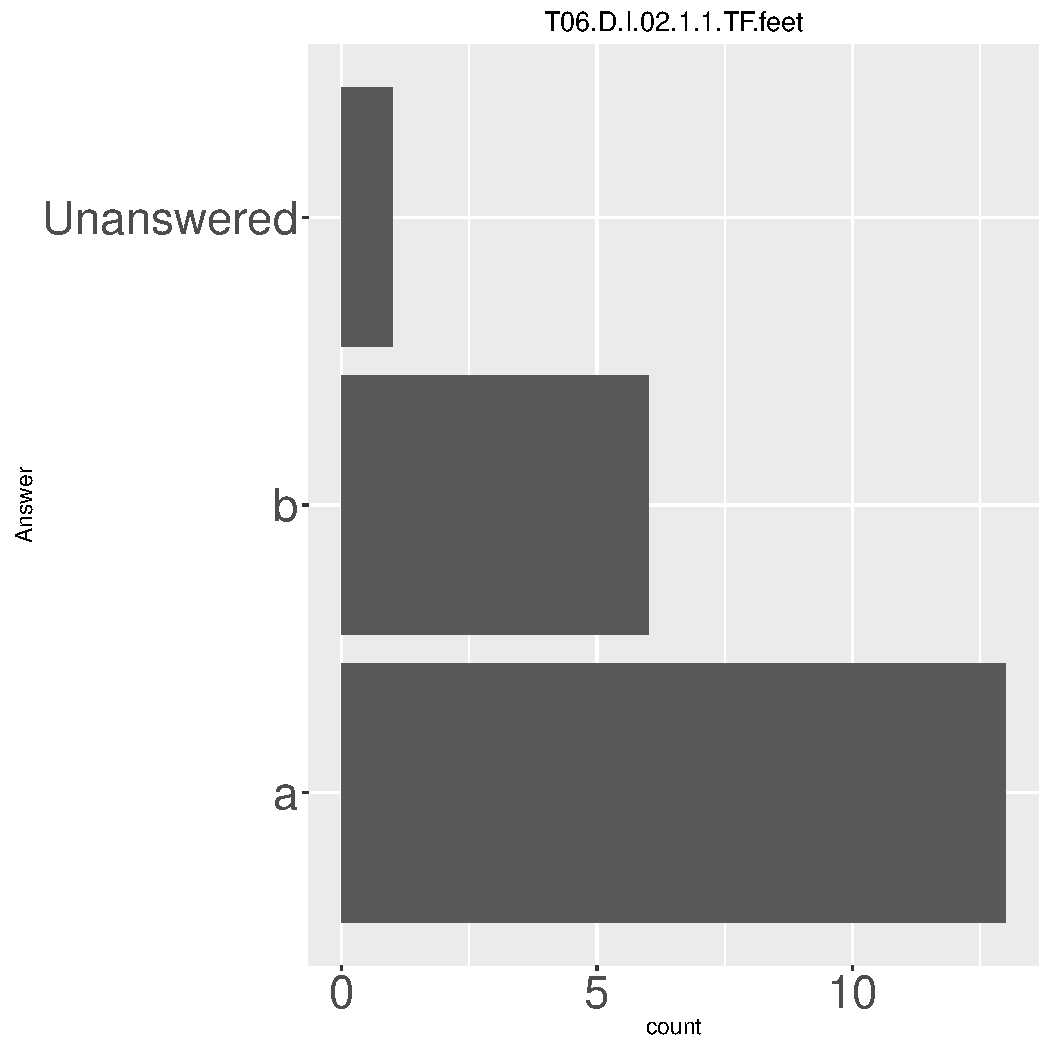
\includegraphics[width=.45\linewidth]{Topic06_AB_21_answer} 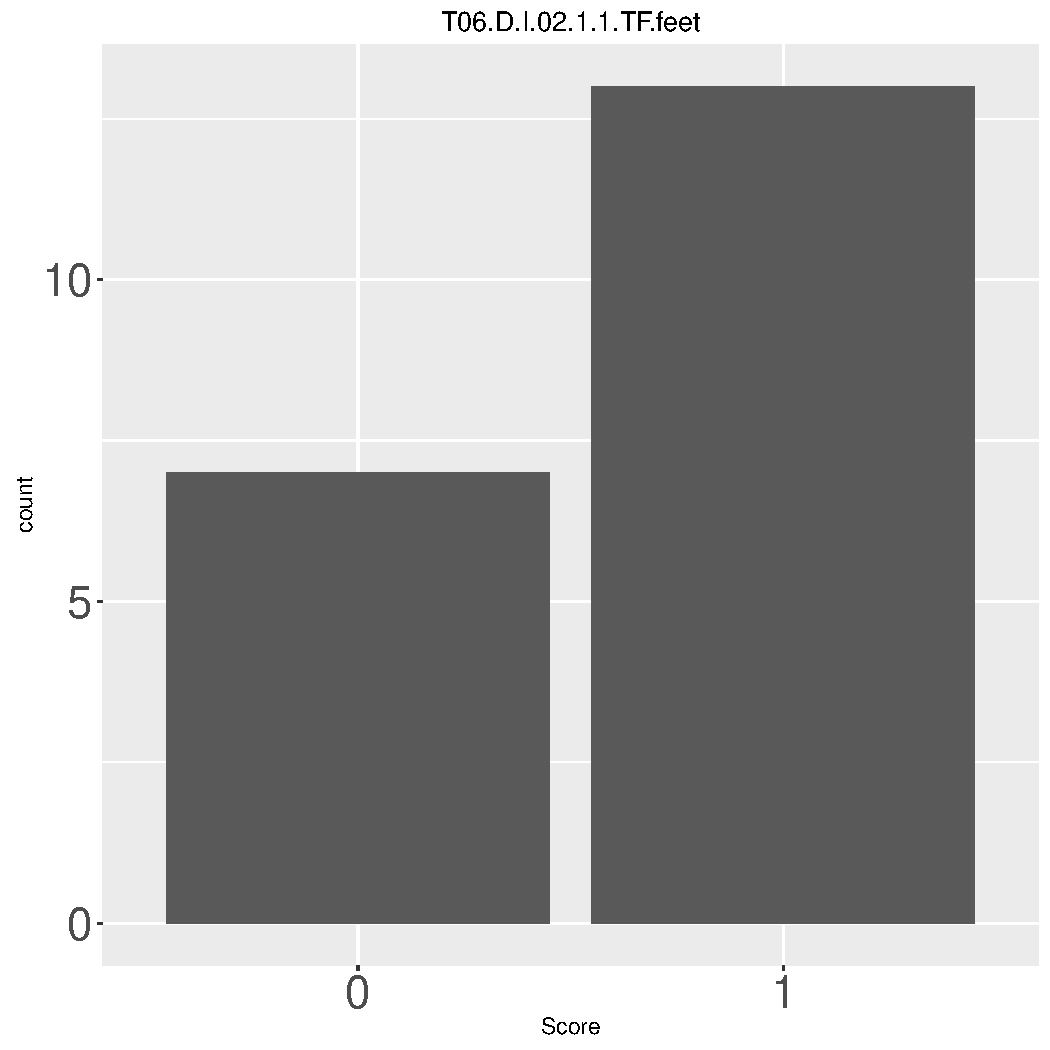
\includegraphics[width=.45\linewidth]{Topic06_AB_21_score} \end{center} 

\begin{center}% latex table generated in R 3.2.2 by xtable 1.8-0 package
% Thu Jan 21 00:33:34 2016
\begin{tabular}{lr}
  \hline
Answer & Count \\ 
  \hline
a &  13 \\ 
  b &   6 \\ 
  Unanswered &   1 \\ 
   \hline
\end{tabular}
~~~~~~~~% latex table generated in R 3.2.2 by xtable 1.8-0 package
% Thu Jan 21 00:33:34 2016
\begin{tabular}{lr}
  \hline
Summary & Value \\ 
  \hline
Mean & 0.65 \\ 
  Std.dev & 0.49 \\ 
  Min & 0.00 \\ 
  Median & 1.00 \\ 
  Max & 1.00 \\ 
   \hline
\end{tabular}
\end{center}\newpage\marginnote{

 Below is the distribution of low temperatures (in degrees F) for 52 cities in the U.S. Based on the output, it is reasonable to model the distribution of low temperature for these cities with a normal distribution. 

}



\vspace{5cm}\begin{marginfigure}\includegraphics[width=0.98\linewidth]{/Users/lindz/ePort/inst/extdata/KeyFiles/Topic06.Questions_files/image004}\end{marginfigure}\marginnote{

 *a. True



b. False 

}\vspace{-5cm}\pdfbookmark[2]{T06.D.I.02.1.1.TF.lowtemp}{T06.D.I.02.1.1.TF.lowtemp} (22) Question "T06.D.I.02.1.1.TF.lowtemp" is given on the right. This question was selected from the question set with a frequency of 0.5. The question was administered to 30 out of the total of 50 students. The average score was 0.63 out of 1.

 (Back to the question summary Table \ref{tab:summary_question}.)

\begin{center} \includegraphics[width=.45\linewidth]{Topic06_AB_22_answer} \includegraphics[width=.45\linewidth]{Topic06_AB_22_score} \end{center} 

\begin{center}% latex table generated in R 3.2.2 by xtable 1.8-0 package
% Thu Jan 21 00:33:35 2016
\begin{tabular}{lr}
  \hline
Answer & Count \\ 
  \hline
a &  19 \\ 
  b &  10 \\ 
  Unanswered &   1 \\ 
   \hline
\end{tabular}
~~~~~~~~% latex table generated in R 3.2.2 by xtable 1.8-0 package
% Thu Jan 21 00:33:35 2016
\begin{tabular}{lr}
  \hline
Summary & Value \\ 
  \hline
Mean & 0.63 \\ 
  Std.dev & 0.49 \\ 
  Min & 0.00 \\ 
  Median & 1.00 \\ 
  Max & 1.00 \\ 
   \hline
\end{tabular}
\end{center}\newpage\marginnote{

 The distribution of the gain of 120 different amplifiers is depicted below.



Based on the output, it is reasonable to model the distribution of amplifier values with a normal distribution. 

}



\vspace{5cm}\begin{marginfigure}\includegraphics[width=0.98\linewidth]{/Users/lindz/ePort/inst/extdata/KeyFiles/Topic06.Questions_files/image006}\end{marginfigure}\marginnote{

 a. True



*b. False 

}\vspace{-5cm}\pdfbookmark[2]{T06.D.J.04.1.1.TF.gain}{T06.D.J.04.1.1.TF.gain} (23) Question "T06.D.J.04.1.1.TF.gain" is given on the right. This question was selected from the question set with a frequency of 0.25. The question was administered to 10 out of the total of 50 students. The average score was 0.6 out of 1.

 (Back to the question summary Table \ref{tab:summary_question}.)

\begin{center} \includegraphics[width=.45\linewidth]{Topic06_AB_23_answer} \includegraphics[width=.45\linewidth]{Topic06_AB_23_score} \end{center} 

\begin{center}% latex table generated in R 3.2.2 by xtable 1.8-0 package
% Thu Jan 21 00:33:36 2016
\begin{tabular}{lr}
  \hline
Answer & Count \\ 
  \hline
b &   6 \\ 
  a &   3 \\ 
  Unanswered &   1 \\ 
   \hline
\end{tabular}
~~~~~~~~% latex table generated in R 3.2.2 by xtable 1.8-0 package
% Thu Jan 21 00:33:36 2016
\begin{tabular}{lr}
  \hline
Summary & Value \\ 
  \hline
Mean & 0.60 \\ 
  Std.dev & 0.52 \\ 
  Min & 0.00 \\ 
  Median & 1.00 \\ 
  Max & 1.00 \\ 
   \hline
\end{tabular}
\end{center}\newpage\marginnote{

 The distribution of estimated highway miles per gallon (mpg) for various makes and models of cars is given below. Based on the output, it is reasonable to model the distribution of highway mpg values with a normal distribution. 

}



\vspace{5cm}\begin{marginfigure}\includegraphics[width=0.98\linewidth]{/Users/lindz/ePort/inst/extdata/KeyFiles/Topic06.Questions_files/image008}\end{marginfigure}\marginnote{

 a. True



*b. False 

}\vspace{-5cm}\pdfbookmark[2]{T06.D.J.04.1.1.TF.mpg}{T06.D.J.04.1.1.TF.mpg} (24) Question "T06.D.J.04.1.1.TF.mpg" is given on the right. This question was selected from the question set with a frequency of 0.25. The question was administered to 6 out of the total of 50 students. The average score was 0.83 out of 1.

 (Back to the question summary Table \ref{tab:summary_question}.)

\begin{center} \includegraphics[width=.45\linewidth]{Topic06_AB_24_answer} \includegraphics[width=.45\linewidth]{Topic06_AB_24_score} \end{center} 

\begin{center}% latex table generated in R 3.2.2 by xtable 1.8-0 package
% Thu Jan 21 00:33:37 2016
\begin{tabular}{lr}
  \hline
Answer & Count \\ 
  \hline
b &   5 \\ 
  a &   1 \\ 
   \hline
\end{tabular}
~~~~~~~~% latex table generated in R 3.2.2 by xtable 1.8-0 package
% Thu Jan 21 00:33:37 2016
\begin{tabular}{lr}
  \hline
Summary & Value \\ 
  \hline
Mean & 0.83 \\ 
  Std.dev & 0.41 \\ 
  Min & 0.00 \\ 
  Median & 1.00 \\ 
  Max & 1.00 \\ 
   \hline
\end{tabular}
\end{center}\newpage\marginnote{

 A blowhole is a hole in a cliff that produces eruptions of water when the ocean swell hits the cliff. Below are 40 times (in seconds) between eruptions for the Kiama blowhole in Australia.



Based on the output, it is reasonable to model the distribution of times between eruptions with a normal distribution. 

}



\vspace{6cm}\begin{marginfigure}\includegraphics[width=0.98\linewidth]{/Users/lindz/ePort/inst/extdata/KeyFiles/Topic06.Questions_files/image010}\end{marginfigure}\marginnote{

 a. True



*b. False 

}\vspace{-6cm}\pdfbookmark[2]{T06.D.J.04.1.1.TF.blowhole}{T06.D.J.04.1.1.TF.blowhole} (25) Question "T06.D.J.04.1.1.TF.blowhole" is given on the right. This question was selected from the question set with a frequency of 0.25. The question was administered to 14 out of the total of 50 students. The average score was 0.5 out of 1.

 (Back to the question summary Table \ref{tab:summary_question}.)

\begin{center} \includegraphics[width=.45\linewidth]{Topic06_AB_25_answer} \includegraphics[width=.45\linewidth]{Topic06_AB_25_score} \end{center} 

\begin{center}% latex table generated in R 3.2.2 by xtable 1.8-0 package
% Thu Jan 21 00:33:38 2016
\begin{tabular}{lr}
  \hline
Answer & Count \\ 
  \hline
a &   7 \\ 
  b &   7 \\ 
   \hline
\end{tabular}
~~~~~~~~% latex table generated in R 3.2.2 by xtable 1.8-0 package
% Thu Jan 21 00:33:38 2016
\begin{tabular}{lr}
  \hline
Summary & Value \\ 
  \hline
Mean & 0.50 \\ 
  Std.dev & 0.52 \\ 
  Min & 0.00 \\ 
  Median & 0.50 \\ 
  Max & 1.00 \\ 
   \hline
\end{tabular}
\end{center}\newpage\marginnote{

 A random sample of 120 students was selected from those students who completed the Stat 101 survey over the last 2 years. The survey asked the number of music CDs owned by each of these students. The histogram of the number of music CDs owned by the students is shown below. Based on the output, it is reasonable to model the distribution of the number of CDs owned by Stat 101 students with a normal distribution. 

}



\vspace{7cm}\begin{marginfigure}\includegraphics[width=0.98\linewidth]{/Users/lindz/ePort/inst/extdata/KeyFiles/Topic06.Questions_files/image012}\end{marginfigure}\marginnote{

 a. True



*b. False 

}\vspace{-7cm}\pdfbookmark[2]{T06.D.J.04.1.1.TF.CDs}{T06.D.J.04.1.1.TF.CDs} (26) Question "T06.D.J.04.1.1.TF.CDs" is given on the right. This question was selected from the question set with a frequency of 0.25. The question was administered to 20 out of the total of 50 students. The average score was 0.55 out of 1.

 (Back to the question summary Table \ref{tab:summary_question}.)

\begin{center} \includegraphics[width=.45\linewidth]{Topic06_AB_26_answer} \includegraphics[width=.45\linewidth]{Topic06_AB_26_score} \end{center} 

\begin{center}% latex table generated in R 3.2.2 by xtable 1.8-0 package
% Thu Jan 21 00:33:38 2016
\begin{tabular}{lr}
  \hline
Answer & Count \\ 
  \hline
b &  11 \\ 
  a &   7 \\ 
  Unanswered &   2 \\ 
   \hline
\end{tabular}
~~~~~~~~% latex table generated in R 3.2.2 by xtable 1.8-0 package
% Thu Jan 21 00:33:38 2016
\begin{tabular}{lr}
  \hline
Summary & Value \\ 
  \hline
Mean & 0.55 \\ 
  Std.dev & 0.51 \\ 
  Min & 0.00 \\ 
  Median & 1.00 \\ 
  Max & 1.00 \\ 
   \hline
\end{tabular}
\end{center}\newpage\marginnote{

 Fill in the blank with the correct number: Assume the length of female humpback whales can be modeled with a normal distribution with a mean of 13.7 meters and a standard deviation of 0.5 meters. According to the Empirical Rule or 68-95-99.7 Rule, \_\_\_\_\_\_\_ percent of female humpback whales will have a length between 13.2 meters and 14.2 meters.



Correct Answer(s):



a. 68



b. 68\% 

}\pdfbookmark[2]{T06.E.K.09.3.1.FB.whale1}{T06.E.K.09.3.1.FB.whale1} (27) Question "T06.E.K.09.3.1.FB.whale1" is given on the right. This question was selected from the question set with a frequency of 0.33. The question was administered to 19 out of the total of 50 students. The average score was 0.21 out of 1.

 (Back to the question summary Table \ref{tab:summary_question}.)

\begin{center} \includegraphics[width=.45\linewidth]{Topic06_AB_27_answer} \includegraphics[width=.45\linewidth]{Topic06_AB_27_score} \end{center} 

\begin{center}% latex table generated in R 3.2.2 by xtable 1.8-0 package
% Thu Jan 21 00:33:39 2016
\begin{tabular}{lr}
  \hline
Answer & Count \\ 
  \hline
95 &   4 \\ 
  a &   4 \\ 
  99.7 &   2 \\ 
  Unanswered &   2 \\ 
  23.1 &   1 \\ 
  3 &   1 \\ 
  34 &   1 \\ 
  35 &   1 \\ 
  68.0 &   1 \\ 
  95.0 &   1 \\ 
  99.70 &   1 \\ 
   \hline
\end{tabular}
~~~~~~~~% latex table generated in R 3.2.2 by xtable 1.8-0 package
% Thu Jan 21 00:33:39 2016
\begin{tabular}{lr}
  \hline
Summary & Value \\ 
  \hline
Mean & 0.21 \\ 
  Std.dev & 0.42 \\ 
  Min & 0.00 \\ 
  Median & 0.00 \\ 
  Max & 1.00 \\ 
   \hline
\end{tabular}
\end{center}\newpage\marginnote{

 Fill in the blank with the correct number: Assume the length of female humpback whales can be modeled with a normal distribution with a mean of 13.7 meters and a standard deviation of 0.5 meters. According to the Empirical Rule or 68-95-99.7 Rule, \_\_\_\_\_\_\_ percent of female humpback whales will have a length between 12.7 meters and 14.7 meters.



Correct Answer(s):



a. 95



b. 95\% 

}\pdfbookmark[2]{T06.E.K.09.3.1.FB.whale2}{T06.E.K.09.3.1.FB.whale2} (28) Question "T06.E.K.09.3.1.FB.whale2" is given on the right. This question was selected from the question set with a frequency of 0.33. The question was administered to 18 out of the total of 50 students. The average score was 0 out of 1.

 (Back to the question summary Table \ref{tab:summary_question}.)

\begin{center} \includegraphics[width=.45\linewidth]{Topic06_AB_28_answer} \includegraphics[width=.45\linewidth]{Topic06_AB_28_score} \end{center} 

\begin{center}% latex table generated in R 3.2.2 by xtable 1.8-0 package
% Thu Jan 21 00:33:40 2016
\begin{tabular}{lr}
  \hline
Answer & Count \\ 
  \hline
68 &   5 \\ 
  23 &   2 \\ 
  99.7 &   2 \\ 
  Unanswered &   2 \\ 
  1 &   1 \\ 
  1.34 &   1 \\ 
  10\% &   1 \\ 
  12 &   1 \\ 
  3 &   1 \\ 
  34 &   1 \\ 
  45 &   1 \\ 
   \hline
\end{tabular}
~~~~~~~~% latex table generated in R 3.2.2 by xtable 1.8-0 package
% Thu Jan 21 00:33:40 2016
\begin{tabular}{lr}
  \hline
Summary & Value \\ 
  \hline
Mean & 0.00 \\ 
  Std.dev & 0.00 \\ 
  Min & 0.00 \\ 
  Median & 0.00 \\ 
  Max & 0.00 \\ 
   \hline
\end{tabular}
\end{center}\newpage\marginnote{

 Fill in the blank with the correct number: Assume the length of female humpback whales can be modeled with a normal distribution with a mean of 13.7 meters and a standard deviation of 0.5 meters. According to the Empirical Rule or 68-95-99.7 Rule, \_\_\_\_\_\_\_ percent of female humpback whales will have a length between 12.2 meters and 15.2 meters.



Correct Answer(s):



a. 99.7



b. 99.7\% 

}\pdfbookmark[2]{T06.E.K.09.3.1.FB.whale3}{T06.E.K.09.3.1.FB.whale3} (29) Question "T06.E.K.09.3.1.FB.whale3" is given on the right. This question was selected from the question set with a frequency of 0.33. The question was administered to 14 out of the total of 50 students. The average score was 0 out of 1.

 (Back to the question summary Table \ref{tab:summary_question}.)

\begin{center} \includegraphics[width=.45\linewidth]{Topic06_AB_29_answer} \includegraphics[width=.45\linewidth]{Topic06_AB_29_score} \end{center} 

\begin{center}% latex table generated in R 3.2.2 by xtable 1.8-0 package
% Thu Jan 21 00:33:40 2016
\begin{tabular}{lr}
  \hline
Answer & Count \\ 
  \hline
23 &   2 \\ 
  95 &   2 \\ 
  95.0 &   2 \\ 
  Unanswered &   2 \\ 
  23.5 &   1 \\ 
  24 &   1 \\ 
  25 &   1 \\ 
  67 &   1 \\ 
  68 &   1 \\ 
  92\% &   1 \\ 
   \hline
\end{tabular}
~~~~~~~~% latex table generated in R 3.2.2 by xtable 1.8-0 package
% Thu Jan 21 00:33:41 2016
\begin{tabular}{lr}
  \hline
Summary & Value \\ 
  \hline
Mean & 0.00 \\ 
  Std.dev & 0.00 \\ 
  Min & 0.00 \\ 
  Median & 0.00 \\ 
  Max & 0.00 \\ 
   \hline
\end{tabular}
\end{center}\newpage\marginnote{

 Fill in the blank with the correct number: Assume the weight of a certain breed of cow can be modeled with a normal distribution with a mean of 750 kg and a standard deviation of 30 kg. According to the Empirical Rule or 68-95-99.7 Rule, \_\_\_\_\_\_\_\_\_ percent of cows from this breed will weigh between 720 kg and 780 kg.



Correct Answer(s):



a. 68



b. 68\% 

}\pdfbookmark[2]{T06.E.K.09.3.1.FB.cow1}{T06.E.K.09.3.1.FB.cow1} (30) Question "T06.E.K.09.3.1.FB.cow1" is given on the right. This question was selected from the question set with a frequency of 0.33. The question was administered to 12 out of the total of 50 students. The average score was 0 out of 1.

 (Back to the question summary Table \ref{tab:summary_question}.)

\begin{center} \includegraphics[width=.45\linewidth]{Topic06_AB_30_answer} \includegraphics[width=.45\linewidth]{Topic06_AB_30_score} \end{center} 

\begin{center}% latex table generated in R 3.2.2 by xtable 1.8-0 package
% Thu Jan 21 00:33:41 2016
\begin{tabular}{lr}
  \hline
Answer & Count \\ 
  \hline
1 &   1 \\ 
  12 &   1 \\ 
  2.53 &   1 \\ 
  24 &   1 \\ 
  3 &   1 \\ 
  34 &   1 \\ 
  4 &   1 \\ 
  435 &   1 \\ 
  45 &   1 \\ 
  54 &   1 \\ 
  99 &   1 \\ 
  Unanswered &   1 \\ 
   \hline
\end{tabular}
~~~~~~~~% latex table generated in R 3.2.2 by xtable 1.8-0 package
% Thu Jan 21 00:33:41 2016
\begin{tabular}{lr}
  \hline
Summary & Value \\ 
  \hline
Mean & 0.00 \\ 
  Std.dev & 0.00 \\ 
  Min & 0.00 \\ 
  Median & 0.00 \\ 
  Max & 0.00 \\ 
   \hline
\end{tabular}
\end{center}\newpage\marginnote{

 Fill in the blank with the correct number: Assume the weight of a certain breed of cow can be modeled with a normal distribution with a mean of 750 kg and a standard deviation of 30 kg. According to the Empirical Rule or 68-95-99.7 Rule, \_\_\_\_\_\_\_\_\_ percent of cows from this breed will weigh between 690 kg and 810 kg.



Correct Answer(s):



a. 95



b. 95\% 

}\pdfbookmark[2]{T06.E.K.09.3.1.FB.cow2}{T06.E.K.09.3.1.FB.cow2} (31) Question "T06.E.K.09.3.1.FB.cow2" is given on the right. This question was selected from the question set with a frequency of 0.33. The question was administered to 18 out of the total of 50 students. The average score was 0.06 out of 1.

 (Back to the question summary Table \ref{tab:summary_question}.)

\begin{center} \includegraphics[width=.45\linewidth]{Topic06_AB_31_answer} \includegraphics[width=.45\linewidth]{Topic06_AB_31_score} \end{center} 

\begin{center}% latex table generated in R 3.2.2 by xtable 1.8-0 package
% Thu Jan 21 00:33:42 2016
\begin{tabular}{lr}
  \hline
Answer & Count \\ 
  \hline
68.0 &   3 \\ 
  99.7 &   3 \\ 
  68 &   2 \\ 
  Unanswered &   2 \\ 
  2 &   1 \\ 
  23 &   1 \\ 
  234 &   1 \\ 
  3 &   1 \\ 
  45 &   1 \\ 
  56 &   1 \\ 
  67 &   1 \\ 
  a &   1 \\ 
   \hline
\end{tabular}
~~~~~~~~% latex table generated in R 3.2.2 by xtable 1.8-0 package
% Thu Jan 21 00:33:42 2016
\begin{tabular}{lr}
  \hline
Summary & Value \\ 
  \hline
Mean & 0.06 \\ 
  Std.dev & 0.24 \\ 
  Min & 0.00 \\ 
  Median & 0.00 \\ 
  Max & 1.00 \\ 
   \hline
\end{tabular}
\end{center}\newpage\marginnote{

 Fill in the blank with the correct number: Assume the weight of a certain breed of cow can be modeled with a normal distribution with a mean of 750 kg and a standard deviation of 30 kg. According to the Empirical Rule or 68-95-99.7 Rule, \_\_\_\_\_\_\_\_\_ percent of cows from this breed will weigh between 660 kg and 840 kg.



Correct Answer(s):



a. 99.7



b. 99.7\% 

}\pdfbookmark[2]{T06.E.K.09.3.1.FB.cow3}{T06.E.K.09.3.1.FB.cow3} (32) Question "T06.E.K.09.3.1.FB.cow3" is given on the right. This question was selected from the question set with a frequency of 0.33. The question was administered to 17 out of the total of 50 students. The average score was 0.12 out of 1.

 (Back to the question summary Table \ref{tab:summary_question}.)

\begin{center} \includegraphics[width=.45\linewidth]{Topic06_AB_32_answer} \includegraphics[width=.45\linewidth]{Topic06_AB_32_score} \end{center} 

\begin{center}% latex table generated in R 3.2.2 by xtable 1.8-0 package
% Thu Jan 21 00:33:43 2016
\begin{tabular}{lr}
  \hline
Answer & Count \\ 
  \hline
95 &   7 \\ 
  45 &   2 \\ 
  a &   2 \\ 
  32 &   1 \\ 
  34 &   1 \\ 
  35 &   1 \\ 
  6 &   1 \\ 
  85\% &   1 \\ 
  95.0 &   1 \\ 
   \hline
\end{tabular}
~~~~~~~~% latex table generated in R 3.2.2 by xtable 1.8-0 package
% Thu Jan 21 00:33:43 2016
\begin{tabular}{lr}
  \hline
Summary & Value \\ 
  \hline
Mean & 0.12 \\ 
  Std.dev & 0.33 \\ 
  Min & 0.00 \\ 
  Median & 0.00 \\ 
  Max & 1.00 \\ 
   \hline
\end{tabular}
\end{center}\newpage\marginnote{

 Fill in the blank with the correct number: Assume the lifespan of light bulbs manufactured by Bright Inc. can be modeled with a normal distribution with a mean of 300 days and a standard deviation of 40 days. According to the Empirical Rule or 68-95-99.7 Rule, \_\_\_\_\_\_\_\_\_\_ percent of light bulbs made by Bright Inc. will last between 260 and 340 days.



Correct Answer(s):



a. 68



b. 68\% 

}\pdfbookmark[2]{T06.E.K.09.3.1.FB.bulbs1}{T06.E.K.09.3.1.FB.bulbs1} (33) Question "T06.E.K.09.3.1.FB.bulbs1" is given on the right. This question was selected from the question set with a frequency of 0.33. The question was administered to 16 out of the total of 50 students. The average score was 0.31 out of 1.

 (Back to the question summary Table \ref{tab:summary_question}.)

\begin{center} \includegraphics[width=.45\linewidth]{Topic06_AB_33_answer} \includegraphics[width=.45\linewidth]{Topic06_AB_33_score} \end{center} 

\begin{center}% latex table generated in R 3.2.2 by xtable 1.8-0 package
% Thu Jan 21 00:33:43 2016
\begin{tabular}{lr}
  \hline
Answer & Count \\ 
  \hline
99.7 &   6 \\ 
  a &   5 \\ 
  124 &   1 \\ 
  3 &   1 \\ 
  68.0 &   1 \\ 
  95.0 &   1 \\ 
  Unanswered &   1 \\ 
   \hline
\end{tabular}
~~~~~~~~% latex table generated in R 3.2.2 by xtable 1.8-0 package
% Thu Jan 21 00:33:43 2016
\begin{tabular}{lr}
  \hline
Summary & Value \\ 
  \hline
Mean & 0.31 \\ 
  Std.dev & 0.48 \\ 
  Min & 0.00 \\ 
  Median & 0.00 \\ 
  Max & 1.00 \\ 
   \hline
\end{tabular}
\end{center}\newpage\marginnote{

 Fill in the blank with the correct number: Assume the lifespan of light bulbs manufactured by Bright Inc. can be modeled with a normal distribution with a mean of 300 days and a standard deviation of 40 days. According to the Empirical Rule or 68-95-99.7 Rule, \_\_\_\_\_\_\_\_\_\_ percent of light bulbs made by Bright Inc. will last between 220 and 380 days.



Correct Answer(s):



a. 95



b. 95\% 

}\pdfbookmark[2]{T06.E.K.09.3.1.FB.bulbs2}{T06.E.K.09.3.1.FB.bulbs2} (34) Question "T06.E.K.09.3.1.FB.bulbs2" is given on the right. This question was selected from the question set with a frequency of 0.33. The question was administered to 17 out of the total of 50 students. The average score was 0.06 out of 1.

 (Back to the question summary Table \ref{tab:summary_question}.)

\begin{center} \includegraphics[width=.45\linewidth]{Topic06_AB_34_answer} \includegraphics[width=.45\linewidth]{Topic06_AB_34_score} \end{center} 

\begin{center}% latex table generated in R 3.2.2 by xtable 1.8-0 package
% Thu Jan 21 00:33:44 2016
\begin{tabular}{lr}
  \hline
Answer & Count \\ 
  \hline
45 &   3 \\ 
  99.7 &   3 \\ 
  68 &   2 \\ 
  1 &   1 \\ 
  13 &   1 \\ 
  23 &   1 \\ 
  32 &   1 \\ 
  34 &   1 \\ 
  35 &   1 \\ 
  67 &   1 \\ 
  95.0 &   1 \\ 
  a &   1 \\ 
   \hline
\end{tabular}
~~~~~~~~% latex table generated in R 3.2.2 by xtable 1.8-0 package
% Thu Jan 21 00:33:44 2016
\begin{tabular}{lr}
  \hline
Summary & Value \\ 
  \hline
Mean & 0.06 \\ 
  Std.dev & 0.24 \\ 
  Min & 0.00 \\ 
  Median & 0.00 \\ 
  Max & 1.00 \\ 
   \hline
\end{tabular}
\end{center}\newpage\marginnote{

 Fill in the blank with the correct number: Assume the lifespan of light bulbs manufactured by Bright Inc. can be modeled with a normal distribution with a mean of 300 days and a standard deviation of 40 days. According to the Empirical Rule or 68-95-99.7 Rule, \_\_\_\_\_\_\_\_\_\_ percent of light bulbs made by Bright Inc. will last between 180 and 420 days.



Correct Answer(s):



a. 99.7



b. 99.7\% 

}\pdfbookmark[2]{T06.E.K.09.3.1.FB.bulbs3}{T06.E.K.09.3.1.FB.bulbs3} (35) Question "T06.E.K.09.3.1.FB.bulbs3" is given on the right. This question was selected from the question set with a frequency of 0.33. The question was administered to 19 out of the total of 50 students. The average score was 0.11 out of 1.

 (Back to the question summary Table \ref{tab:summary_question}.)

\begin{center} \includegraphics[width=.45\linewidth]{Topic06_AB_35_answer} \includegraphics[width=.45\linewidth]{Topic06_AB_35_score} \end{center} 

\begin{center}% latex table generated in R 3.2.2 by xtable 1.8-0 package
% Thu Jan 21 00:33:45 2016
\begin{tabular}{lr}
  \hline
Answer & Count \\ 
  \hline
95 &   5 \\ 
  68 &   4 \\ 
  a &   2 \\ 
  Unanswered &   2 \\ 
  14 &   1 \\ 
  23 &   1 \\ 
  25 &   1 \\ 
  3 &   1 \\ 
  5 &   1 \\ 
  95.0 &   1 \\ 
   \hline
\end{tabular}
~~~~~~~~% latex table generated in R 3.2.2 by xtable 1.8-0 package
% Thu Jan 21 00:33:45 2016
\begin{tabular}{lr}
  \hline
Summary & Value \\ 
  \hline
Mean & 0.11 \\ 
  Std.dev & 0.32 \\ 
  Min & 0.00 \\ 
  Median & 0.00 \\ 
  Max & 1.00 \\ 
   \hline
\end{tabular}
\end{center}\newpage\marginnote{

 Assume the distribution of the height of adult females can be modeled with a normal distribution with mean 66 inches and standard deviation 3 inches. According to the Empirical Rule or 68-95-99.7 Rule, the center 99.7\% of all women will have heights between \_\_\_\_\_\_\_ and 75 inches.



a. 60



*b. 57



c. 63



d. 66 

}\pdfbookmark[2]{T06.E.L.09.3.1.MC.heights1}{T06.E.L.09.3.1.MC.heights1} (36) Question "T06.E.L.09.3.1.MC.heights1" is given on the right. This question was selected from the question set with a frequency of 0.33. The question was administered to 19 out of the total of 50 students. The average score was 0.16 out of 1.

 (Back to the question summary Table \ref{tab:summary_question}.)

\begin{center} \includegraphics[width=.45\linewidth]{Topic06_AB_36_answer} \includegraphics[width=.45\linewidth]{Topic06_AB_36_score} \end{center} 

\begin{center}% latex table generated in R 3.2.2 by xtable 1.8-0 package
% Thu Jan 21 00:33:46 2016
\begin{tabular}{lr}
  \hline
Answer & Count \\ 
  \hline
d &   7 \\ 
  a &   6 \\ 
  b &   3 \\ 
  c &   3 \\ 
   \hline
\end{tabular}
~~~~~~~~% latex table generated in R 3.2.2 by xtable 1.8-0 package
% Thu Jan 21 00:33:46 2016
\begin{tabular}{lr}
  \hline
Summary & Value \\ 
  \hline
Mean & 0.16 \\ 
  Std.dev & 0.37 \\ 
  Min & 0.00 \\ 
  Median & 0.00 \\ 
  Max & 1.00 \\ 
   \hline
\end{tabular}
\end{center}\newpage\marginnote{

 Assume the distribution of the height of adult females can be modeled with a normal distribution with mean 66 inches and standard deviation 3 inches. According to the Empirical Rule or 68-95-99.7 Rule, the center 68\% of all women will have heights between \_\_\_\_\_\_\_ and 69 inches.



a. 60



b. 57



*c. 63



d. 66 

}\pdfbookmark[2]{T06.E.L.09.3.1.MC.heights2}{T06.E.L.09.3.1.MC.heights2} (37) Question "T06.E.L.09.3.1.MC.heights2" is given on the right. This question was selected from the question set with a frequency of 0.33. The question was administered to 18 out of the total of 50 students. The average score was 0.06 out of 1.

 (Back to the question summary Table \ref{tab:summary_question}.)

\begin{center} \includegraphics[width=.45\linewidth]{Topic06_AB_37_answer} \includegraphics[width=.45\linewidth]{Topic06_AB_37_score} \end{center} 

\begin{center}% latex table generated in R 3.2.2 by xtable 1.8-0 package
% Thu Jan 21 00:33:46 2016
\begin{tabular}{lr}
  \hline
Answer & Count \\ 
  \hline
a &   6 \\ 
  d &   6 \\ 
  b &   4 \\ 
  c &   1 \\ 
  Unanswered &   1 \\ 
   \hline
\end{tabular}
~~~~~~~~% latex table generated in R 3.2.2 by xtable 1.8-0 package
% Thu Jan 21 00:33:46 2016
\begin{tabular}{lr}
  \hline
Summary & Value \\ 
  \hline
Mean & 0.06 \\ 
  Std.dev & 0.24 \\ 
  Min & 0.00 \\ 
  Median & 0.00 \\ 
  Max & 1.00 \\ 
   \hline
\end{tabular}
\end{center}\newpage\marginnote{

 Assume the distribution of the height of adult females can be modeled with a normal distribution with mean 66 inches and standard deviation 3 inches. According to the Empirical Rule or 68-95-99.7 Rule, the center 95\% of all women will have heights between \_\_\_\_\_\_\_ and 72 inches.



*a. 60



b. 57



c. 63



d. 66 

}\pdfbookmark[2]{T06.E.L.09.3.1.MC.heights3}{T06.E.L.09.3.1.MC.heights3} (38) Question "T06.E.L.09.3.1.MC.heights3" is given on the right. This question was selected from the question set with a frequency of 0.33. The question was administered to 19 out of the total of 50 students. The average score was 0.42 out of 1.

 (Back to the question summary Table \ref{tab:summary_question}.)

\begin{center} \includegraphics[width=.45\linewidth]{Topic06_AB_38_answer} \includegraphics[width=.45\linewidth]{Topic06_AB_38_score} \end{center} 

\begin{center}% latex table generated in R 3.2.2 by xtable 1.8-0 package
% Thu Jan 21 00:33:47 2016
\begin{tabular}{lr}
  \hline
Answer & Count \\ 
  \hline
d &  10 \\ 
  a &   8 \\ 
  Unanswered &   1 \\ 
   \hline
\end{tabular}
~~~~~~~~% latex table generated in R 3.2.2 by xtable 1.8-0 package
% Thu Jan 21 00:33:47 2016
\begin{tabular}{lr}
  \hline
Summary & Value \\ 
  \hline
Mean & 0.42 \\ 
  Std.dev & 0.51 \\ 
  Min & 0.00 \\ 
  Median & 0.00 \\ 
  Max & 1.00 \\ 
   \hline
\end{tabular}
\end{center}\newpage\marginnote{

 Assume the weight of bags of M\&Ms can be modeled with the normal distribution with mean 50 grams and standard deviation 1 gram. According to the Empirical Rule or 68-95-99.7 rule, 99.7\% of all M\&M bags will have weights between \_\_\_\_\_\_\_ and 53 grams.



*a. 47



b. 48



c. 49



d. 50 

}\pdfbookmark[2]{T06.E.L.09.3.1.MC.mm1}{T06.E.L.09.3.1.MC.mm1} (39) Question "T06.E.L.09.3.1.MC.mm1" is given on the right. This question was selected from the question set with a frequency of 0.33. The question was administered to 13 out of the total of 50 students. The average score was 0.08 out of 1.

 (Back to the question summary Table \ref{tab:summary_question}.)

\begin{center} \includegraphics[width=.45\linewidth]{Topic06_AB_39_answer} \includegraphics[width=.45\linewidth]{Topic06_AB_39_score} \end{center} 

\begin{center}% latex table generated in R 3.2.2 by xtable 1.8-0 package
% Thu Jan 21 00:33:48 2016
\begin{tabular}{lr}
  \hline
Answer & Count \\ 
  \hline
b &   4 \\ 
  d &   4 \\ 
  c &   3 \\ 
  a &   1 \\ 
  Unanswered &   1 \\ 
   \hline
\end{tabular}
~~~~~~~~% latex table generated in R 3.2.2 by xtable 1.8-0 package
% Thu Jan 21 00:33:48 2016
\begin{tabular}{lr}
  \hline
Summary & Value \\ 
  \hline
Mean & 0.08 \\ 
  Std.dev & 0.28 \\ 
  Min & 0.00 \\ 
  Median & 0.00 \\ 
  Max & 1.00 \\ 
   \hline
\end{tabular}
\end{center}\newpage\marginnote{

 Assume the weight of bags of M\&Ms can be modeled with the normal distribution with mean 50 grams and standard deviation 1 gram. According to the Empirical Rule or 68-95-99.7 rule, 68\% of all M\&M bags will have weights between \_\_\_\_\_\_\_ and 51 grams.



a. 47



b. 48



*c. 49



d. 50 

}\pdfbookmark[2]{T06.E.L.09.3.1.MC.mm2}{T06.E.L.09.3.1.MC.mm2} (40) Question "T06.E.L.09.3.1.MC.mm2" is given on the right. This question was selected from the question set with a frequency of 0.33. The question was administered to 16 out of the total of 50 students. The average score was 0.31 out of 1.

 (Back to the question summary Table \ref{tab:summary_question}.)

\begin{center} \includegraphics[width=.45\linewidth]{Topic06_AB_40_answer} \includegraphics[width=.45\linewidth]{Topic06_AB_40_score} \end{center} 

\begin{center}% latex table generated in R 3.2.2 by xtable 1.8-0 package
% Thu Jan 21 00:33:48 2016
\begin{tabular}{lr}
  \hline
Answer & Count \\ 
  \hline
d &   6 \\ 
  c &   5 \\ 
  b &   4 \\ 
  a &   1 \\ 
   \hline
\end{tabular}
~~~~~~~~% latex table generated in R 3.2.2 by xtable 1.8-0 package
% Thu Jan 21 00:33:48 2016
\begin{tabular}{lr}
  \hline
Summary & Value \\ 
  \hline
Mean & 0.31 \\ 
  Std.dev & 0.48 \\ 
  Min & 0.00 \\ 
  Median & 0.00 \\ 
  Max & 1.00 \\ 
   \hline
\end{tabular}
\end{center}\newpage\marginnote{

 Assume the weight of bags of M\&Ms can be modeled with the normal distribution with mean 50 grams and standard deviation 1 gram. According to the Empirical Rule or 68-95-99.7 rule, 95\% of all M\&M bags will have weights between \_\_\_\_\_\_\_ and 52 grams.



a. 47



*b. 48



c. 49



d. 50 

}\pdfbookmark[2]{T06.E.L.09.3.1.MC.mm3}{T06.E.L.09.3.1.MC.mm3} (41) Question "T06.E.L.09.3.1.MC.mm3" is given on the right. This question was selected from the question set with a frequency of 0.33. The question was administered to 19 out of the total of 50 students. The average score was 0.26 out of 1.

 (Back to the question summary Table \ref{tab:summary_question}.)

\begin{center} \includegraphics[width=.45\linewidth]{Topic06_AB_41_answer} \includegraphics[width=.45\linewidth]{Topic06_AB_41_score} \end{center} 

\begin{center}% latex table generated in R 3.2.2 by xtable 1.8-0 package
% Thu Jan 21 00:33:49 2016
\begin{tabular}{lr}
  \hline
Answer & Count \\ 
  \hline
d &   7 \\ 
  a &   5 \\ 
  b &   5 \\ 
  c &   2 \\ 
   \hline
\end{tabular}
~~~~~~~~% latex table generated in R 3.2.2 by xtable 1.8-0 package
% Thu Jan 21 00:33:49 2016
\begin{tabular}{lr}
  \hline
Summary & Value \\ 
  \hline
Mean & 0.26 \\ 
  Std.dev & 0.45 \\ 
  Min & 0.00 \\ 
  Median & 0.00 \\ 
  Max & 1.00 \\ 
   \hline
\end{tabular}
\end{center}\newpage\marginnote{

 Assume the distribution of IQ scores for adults can be modeled with a normal distribution with a mean score of 100 points and a standard deviation of 10 points. According to the Empirical Rule or 68-95-99.7 Rule, the middle 95\% of all adults will have an IQ score between 80 and \_\_\_\_\_\_\_ points.



a. 110



b. 100



*c. 120



d. 130 

}\pdfbookmark[2]{T06.E.L.09.3.1.MC.IQ1}{T06.E.L.09.3.1.MC.IQ1} (42) Question "T06.E.L.09.3.1.MC.IQ1" is given on the right. This question was selected from the question set with a frequency of 0.33. The question was administered to 18 out of the total of 50 students. The average score was 0.33 out of 1.

 (Back to the question summary Table \ref{tab:summary_question}.)

\begin{center} \includegraphics[width=.45\linewidth]{Topic06_AB_42_answer} \includegraphics[width=.45\linewidth]{Topic06_AB_42_score} \end{center} 

\begin{center}% latex table generated in R 3.2.2 by xtable 1.8-0 package
% Thu Jan 21 00:33:50 2016
\begin{tabular}{lr}
  \hline
Answer & Count \\ 
  \hline
c &   6 \\ 
  d &   5 \\ 
  a &   4 \\ 
  b &   2 \\ 
  Unanswered &   1 \\ 
   \hline
\end{tabular}
~~~~~~~~% latex table generated in R 3.2.2 by xtable 1.8-0 package
% Thu Jan 21 00:33:50 2016
\begin{tabular}{lr}
  \hline
Summary & Value \\ 
  \hline
Mean & 0.33 \\ 
  Std.dev & 0.49 \\ 
  Min & 0.00 \\ 
  Median & 0.00 \\ 
  Max & 1.00 \\ 
   \hline
\end{tabular}
\end{center}\newpage\marginnote{

 Assume the distribution of IQ scores for adults can be modeled with a normal distribution with a mean score of 100 points and a standard deviation of 10 points. According to the Empirical Rule or 68-95-99.7 Rule, the middle 68\% of all adults will have an IQ score between 90 and \_\_\_\_\_\_\_ points.



*a. 110



b. 100



c. 120



d. 130 

}\pdfbookmark[2]{T06.E.L.09.3.1.MC.IQ2}{T06.E.L.09.3.1.MC.IQ2} (43) Question "T06.E.L.09.3.1.MC.IQ2" is given on the right. This question was selected from the question set with a frequency of 0.33. The question was administered to 13 out of the total of 50 students. The average score was 0.38 out of 1.

 (Back to the question summary Table \ref{tab:summary_question}.)

\begin{center} \includegraphics[width=.45\linewidth]{Topic06_AB_43_answer} \includegraphics[width=.45\linewidth]{Topic06_AB_43_score} \end{center} 

\begin{center}% latex table generated in R 3.2.2 by xtable 1.8-0 package
% Thu Jan 21 00:33:50 2016
\begin{tabular}{lr}
  \hline
Answer & Count \\ 
  \hline
a &   5 \\ 
  c &   4 \\ 
  b &   2 \\ 
  d &   1 \\ 
  Unanswered &   1 \\ 
   \hline
\end{tabular}
~~~~~~~~% latex table generated in R 3.2.2 by xtable 1.8-0 package
% Thu Jan 21 00:33:50 2016
\begin{tabular}{lr}
  \hline
Summary & Value \\ 
  \hline
Mean & 0.38 \\ 
  Std.dev & 0.51 \\ 
  Min & 0.00 \\ 
  Median & 0.00 \\ 
  Max & 1.00 \\ 
   \hline
\end{tabular}
\end{center}\newpage\marginnote{

 Assume the distribution of IQ scores for adults can be modeled with a normal distribution with a mean score of 100 points and a standard deviation of 10 points. According to the Empirical Rule or 68-95-99.7 Rule, the middle 99.7\% of all adults will have an IQ score between 70 and \_\_\_\_\_\_\_ points.



a. 110



b. 100



c. 120



*d. 130 

}\pdfbookmark[2]{T06.E.L.09.3.1.MC.IQ3}{T06.E.L.09.3.1.MC.IQ3} (44) Question "T06.E.L.09.3.1.MC.IQ3" is given on the right. This question was selected from the question set with a frequency of 0.33. The question was administered to 15 out of the total of 50 students. The average score was 0.07 out of 1.

 (Back to the question summary Table \ref{tab:summary_question}.)

\begin{center} \includegraphics[width=.45\linewidth]{Topic06_AB_44_answer} \includegraphics[width=.45\linewidth]{Topic06_AB_44_score} \end{center} 

\begin{center}% latex table generated in R 3.2.2 by xtable 1.8-0 package
% Thu Jan 21 00:33:51 2016
\begin{tabular}{lr}
  \hline
Answer & Count \\ 
  \hline
a &   5 \\ 
  c &   5 \\ 
  b &   4 \\ 
  d &   1 \\ 
   \hline
\end{tabular}
~~~~~~~~% latex table generated in R 3.2.2 by xtable 1.8-0 package
% Thu Jan 21 00:33:51 2016
\begin{tabular}{lr}
  \hline
Summary & Value \\ 
  \hline
Mean & 0.07 \\ 
  Std.dev & 0.26 \\ 
  Min & 0.00 \\ 
  Median & 0.00 \\ 
  Max & 1.00 \\ 
   \hline
\end{tabular}
\end{center}\newpage\marginnote{

 For the remaining questions, use either a z-table or an applet or both to do the calculations. Depending on the method used, the final answer could be subject to a small amount of rounding error. Assume the weight of bags of M\&Ms can be modeled with the normal distribution with mean 50 grams and standard deviation 1 gram. The weight on the label of these M\&M bags is 47.9 grams. What percentage of all M\&M bags have a weight below the label weight?



*a. 1.79\%



b. 98.21\%



c. 1.39\%



d. 2.28\%



e. 97.72\% 

}\pdfbookmark[2]{T06.F.M.05.1.1.MC.mm1}{T06.F.M.05.1.1.MC.mm1} (45) Question "T06.F.M.05.1.1.MC.mm1" is given on the right. This question was selected from the question set with a frequency of 0.2. The question was administered to 19 out of the total of 50 students. The average score was 0.53 out of 1.

 (Back to the question summary Table \ref{tab:summary_question}.)

\begin{center} \includegraphics[width=.45\linewidth]{Topic06_AB_45_answer} \includegraphics[width=.45\linewidth]{Topic06_AB_45_score} \end{center} 

\begin{center}% latex table generated in R 3.2.2 by xtable 1.8-0 package
% Thu Jan 21 00:33:52 2016
\begin{tabular}{lr}
  \hline
Answer & Count \\ 
  \hline
a &  10 \\ 
  d &   4 \\ 
  b &   3 \\ 
  c &   2 \\ 
   \hline
\end{tabular}
~~~~~~~~% latex table generated in R 3.2.2 by xtable 1.8-0 package
% Thu Jan 21 00:33:52 2016
\begin{tabular}{lr}
  \hline
Summary & Value \\ 
  \hline
Mean & 0.53 \\ 
  Std.dev & 0.51 \\ 
  Min & 0.00 \\ 
  Median & 1.00 \\ 
  Max & 1.00 \\ 
   \hline
\end{tabular}
\end{center}\newpage\marginnote{

 For the remaining questions, use either a z-table or an applet or both to do the calculations. Depending on the method used, the final answer could be subject to a small amount of rounding error. Assume the lifespan of light bulbs manufactured by Bright Inc. can be modeled with a normal distribution with a mean of 300 days and a standard deviation of 40 days. What percentage of light bulbs produced by Bright Inc. will survive less than 200 days?



a. 99.38\%



*b. 0.62\%



c. 96.49\%



d. 12.3\%



e. 2.02\% 

}\pdfbookmark[2]{T06.F.M.05.1.1.MC.Bulb1}{T06.F.M.05.1.1.MC.Bulb1} (46) Question "T06.F.M.05.1.1.MC.Bulb1" is given on the right. This question was selected from the question set with a frequency of 0.2. The question was administered to 8 out of the total of 50 students. The average score was 0.25 out of 1.

 (Back to the question summary Table \ref{tab:summary_question}.)

\begin{center} \includegraphics[width=.45\linewidth]{Topic06_AB_46_answer} \includegraphics[width=.45\linewidth]{Topic06_AB_46_score} \end{center} 

\begin{center}% latex table generated in R 3.2.2 by xtable 1.8-0 package
% Thu Jan 21 00:33:53 2016
\begin{tabular}{lr}
  \hline
Answer & Count \\ 
  \hline
b &   2 \\ 
  c &   2 \\ 
  d &   2 \\ 
  e &   2 \\ 
   \hline
\end{tabular}
~~~~~~~~% latex table generated in R 3.2.2 by xtable 1.8-0 package
% Thu Jan 21 00:33:53 2016
\begin{tabular}{lr}
  \hline
Summary & Value \\ 
  \hline
Mean & 0.25 \\ 
  Std.dev & 0.46 \\ 
  Min & 0.00 \\ 
  Median & 0.00 \\ 
  Max & 1.00 \\ 
   \hline
\end{tabular}
\end{center}\newpage\marginnote{

 For the remaining questions, use either a z-table or an applet or both to do the calculations. Depending on the method used, the final answer could be subject to a small amount of rounding error. Assume the distribution of IQ scores for adults can be modeled with a normal distribution with a mean score of 100 points and a standard deviation of 10 points. What percentage of adults have an IQ score of less than 87 points?



*a. 9.68\%



b. 15.15\%



c. 4.46\%



d. 90.32\%



e. 84.85\% 

}\pdfbookmark[2]{T06.F.M.05.1.1.MC.IQ1}{T06.F.M.05.1.1.MC.IQ1} (47) Question "T06.F.M.05.1.1.MC.IQ1" is given on the right. This question was selected from the question set with a frequency of 0.2. The question was administered to 8 out of the total of 50 students. The average score was 0.25 out of 1.

 (Back to the question summary Table \ref{tab:summary_question}.)

\begin{center} \includegraphics[width=.45\linewidth]{Topic06_AB_47_answer} \includegraphics[width=.45\linewidth]{Topic06_AB_47_score} \end{center} 

\begin{center}% latex table generated in R 3.2.2 by xtable 1.8-0 package
% Thu Jan 21 00:33:53 2016
\begin{tabular}{lr}
  \hline
Answer & Count \\ 
  \hline
e &   3 \\ 
  a &   2 \\ 
  b &   2 \\ 
  Unanswered &   1 \\ 
   \hline
\end{tabular}
~~~~~~~~% latex table generated in R 3.2.2 by xtable 1.8-0 package
% Thu Jan 21 00:33:53 2016
\begin{tabular}{lr}
  \hline
Summary & Value \\ 
  \hline
Mean & 0.25 \\ 
  Std.dev & 0.46 \\ 
  Min & 0.00 \\ 
  Median & 0.00 \\ 
  Max & 1.00 \\ 
   \hline
\end{tabular}
\end{center}\newpage\marginnote{

 For the remaining questions, use either a z-table or an applet or both to do the calculations. Depending on the method used, the final answer could be subject to a small amount of rounding error. Assume the length of female humpback whales can be modeled with a normal distribution with a mean of 13.7 meters and a standard deviation of 0.5 meters. What percentage of female humpback whales will be shorter than 13 meters in length?



*a. 8.08\%



b. 91.92\%



c. 14.92\%



d. 85.08\%



e. 0.82\% 

}\pdfbookmark[2]{T06.F.M.05.1.1.MC.Whale1}{T06.F.M.05.1.1.MC.Whale1} (48) Question "T06.F.M.05.1.1.MC.Whale1" is given on the right. This question was selected from the question set with a frequency of 0.2. The question was administered to 7 out of the total of 50 students. The average score was 0.29 out of 1.

 (Back to the question summary Table \ref{tab:summary_question}.)

\begin{center} \includegraphics[width=.45\linewidth]{Topic06_AB_48_answer} \includegraphics[width=.45\linewidth]{Topic06_AB_48_score} \end{center} 

\begin{center}% latex table generated in R 3.2.2 by xtable 1.8-0 package
% Thu Jan 21 00:33:54 2016
\begin{tabular}{lr}
  \hline
Answer & Count \\ 
  \hline
b &   4 \\ 
  a &   2 \\ 
  d &   1 \\ 
   \hline
\end{tabular}
~~~~~~~~% latex table generated in R 3.2.2 by xtable 1.8-0 package
% Thu Jan 21 00:33:54 2016
\begin{tabular}{lr}
  \hline
Summary & Value \\ 
  \hline
Mean & 0.29 \\ 
  Std.dev & 0.49 \\ 
  Min & 0.00 \\ 
  Median & 0.00 \\ 
  Max & 1.00 \\ 
   \hline
\end{tabular}
\end{center}\newpage\marginnote{

 For the remaining questions, use either a z-table or an applet or both to do the calculations. Depending on the method used, the final answer could be subject to a small amount of rounding error. Assume the weight of a certain breed of cow can be modeled with a normal distribution with a mean of 750 kg and a standard deviation of 30 kg. What percentage of cows from this breed will weigh less than 680 kg?



*a. 0.99\%



b. 99.01\%



c. 2.12\%



d. 97.88\%



e. 0.38\% 

}\pdfbookmark[2]{T06.F.M.05.1.1.MC.Cow1}{T06.F.M.05.1.1.MC.Cow1} (49) Question "T06.F.M.05.1.1.MC.Cow1" is given on the right. This question was selected from the question set with a frequency of 0.2. The question was administered to 8 out of the total of 50 students. The average score was 0.25 out of 1.

 (Back to the question summary Table \ref{tab:summary_question}.)

\begin{center} \includegraphics[width=.45\linewidth]{Topic06_AB_49_answer} \includegraphics[width=.45\linewidth]{Topic06_AB_49_score} \end{center} 

\begin{center}% latex table generated in R 3.2.2 by xtable 1.8-0 package
% Thu Jan 21 00:33:55 2016
\begin{tabular}{lr}
  \hline
Answer & Count \\ 
  \hline
a &   2 \\ 
  b &   2 \\ 
  c &   1 \\ 
  d &   1 \\ 
  e &   1 \\ 
  Unanswered &   1 \\ 
   \hline
\end{tabular}
~~~~~~~~% latex table generated in R 3.2.2 by xtable 1.8-0 package
% Thu Jan 21 00:33:55 2016
\begin{tabular}{lr}
  \hline
Summary & Value \\ 
  \hline
Mean & 0.25 \\ 
  Std.dev & 0.46 \\ 
  Min & 0.00 \\ 
  Median & 0.00 \\ 
  Max & 1.00 \\ 
   \hline
\end{tabular}
\end{center}\newpage\marginnote{

 Assume the weight of bags of M\&Ms can be modeled with the normal distribution with mean 50 grams and standard deviation 1 gram. What percentage of all M\&M bags will have a weight below 51.5 grams?



*a. 93.32\%



b. 6.68\%



c. 85.31\%



d. 14.69\%



e. 90.32\% 

}\pdfbookmark[2]{T06.F.N.05.1.1.MC.mm2}{T06.F.N.05.1.1.MC.mm2} (50) Question "T06.F.N.05.1.1.MC.mm2" is given on the right. This question was selected from the question set with a frequency of 0.2. The question was administered to 8 out of the total of 50 students. The average score was 0.38 out of 1.

 (Back to the question summary Table \ref{tab:summary_question}.)

\begin{center} \includegraphics[width=.45\linewidth]{Topic06_AB_50_answer} \includegraphics[width=.45\linewidth]{Topic06_AB_50_score} \end{center} 

\begin{center}% latex table generated in R 3.2.2 by xtable 1.8-0 package
% Thu Jan 21 00:33:55 2016
\begin{tabular}{lr}
  \hline
Answer & Count \\ 
  \hline
a &   3 \\ 
  e &   3 \\ 
  d &   2 \\ 
   \hline
\end{tabular}
~~~~~~~~% latex table generated in R 3.2.2 by xtable 1.8-0 package
% Thu Jan 21 00:33:55 2016
\begin{tabular}{lr}
  \hline
Summary & Value \\ 
  \hline
Mean & 0.38 \\ 
  Std.dev & 0.52 \\ 
  Min & 0.00 \\ 
  Median & 0.00 \\ 
  Max & 1.00 \\ 
   \hline
\end{tabular}
\end{center}\newpage\marginnote{

 Assume the lifespan of light bulbs manufactured by Bright Inc. can be modeled with a normal distribution with a mean of 300 days and a standard deviation of 40 days. What percentage of light bulbs produced by Bright Inc. will survive less than 405 days?



*a. 99.57\%



b. 0.43\%



c. 99.09\%



d. 0.91\%



e. 94.84\% 

}\pdfbookmark[2]{T06.F.N.05.1.1.MC.Bulb2}{T06.F.N.05.1.1.MC.Bulb2} (51) Question "T06.F.N.05.1.1.MC.Bulb2" is given on the right. This question was selected from the question set with a frequency of 0.2. The question was administered to 11 out of the total of 50 students. The average score was 0 out of 1.

 (Back to the question summary Table \ref{tab:summary_question}.)

\begin{center} \includegraphics[width=.45\linewidth]{Topic06_AB_51_answer} \includegraphics[width=.45\linewidth]{Topic06_AB_51_score} \end{center} 

\begin{center}% latex table generated in R 3.2.2 by xtable 1.8-0 package
% Thu Jan 21 00:33:56 2016
\begin{tabular}{lr}
  \hline
Answer & Count \\ 
  \hline
c &   5 \\ 
  d &   4 \\ 
  b &   1 \\ 
  Unanswered &   1 \\ 
   \hline
\end{tabular}
~~~~~~~~% latex table generated in R 3.2.2 by xtable 1.8-0 package
% Thu Jan 21 00:33:56 2016
\begin{tabular}{lr}
  \hline
Summary & Value \\ 
  \hline
Mean & 0.00 \\ 
  Std.dev & 0.00 \\ 
  Min & 0.00 \\ 
  Median & 0.00 \\ 
  Max & 0.00 \\ 
   \hline
\end{tabular}
\end{center}\newpage\marginnote{

 Assume the distribution of IQ scores for adults can be modeled with a normal distribution with a mean score of 100 points and a standard deviation of 10 points. What percentage of adults have an IQ score of less than 107 points?



*a. 75.8\%



b. 24.2\%



c. 72.3\%



d. 85.7\%



e. 14.3\% 

}\pdfbookmark[2]{T06.F.N.05.1.1.MC.IQ2}{T06.F.N.05.1.1.MC.IQ2} (52) Question "T06.F.N.05.1.1.MC.IQ2" is given on the right. This question was selected from the question set with a frequency of 0.2. The question was administered to 11 out of the total of 50 students. The average score was 0.27 out of 1.

 (Back to the question summary Table \ref{tab:summary_question}.)

\begin{center} \includegraphics[width=.45\linewidth]{Topic06_AB_52_answer} \includegraphics[width=.45\linewidth]{Topic06_AB_52_score} \end{center} 

\begin{center}% latex table generated in R 3.2.2 by xtable 1.8-0 package
% Thu Jan 21 00:33:57 2016
\begin{tabular}{lr}
  \hline
Answer & Count \\ 
  \hline
a &   3 \\ 
  e &   3 \\ 
  b &   2 \\ 
  c &   2 \\ 
  d &   1 \\ 
   \hline
\end{tabular}
~~~~~~~~% latex table generated in R 3.2.2 by xtable 1.8-0 package
% Thu Jan 21 00:33:57 2016
\begin{tabular}{lr}
  \hline
Summary & Value \\ 
  \hline
Mean & 0.27 \\ 
  Std.dev & 0.47 \\ 
  Min & 0.00 \\ 
  Median & 0.00 \\ 
  Max & 1.00 \\ 
   \hline
\end{tabular}
\end{center}\newpage\marginnote{

 Assume the length of female humpback whales can be modeled with a normal distribution with a mean of 13.7 meters and a standard deviation of 0.5 meters. What percentage of female humpback whales will be shorter than 14 meters in length?



a. 77.04\%



*b. 72.57\%



c. 27.43\%



d. 68.44\%



e. 22.96\% 

}\pdfbookmark[2]{T06.F.N.05.1.1.MC.Whale2}{T06.F.N.05.1.1.MC.Whale2} (53) Question "T06.F.N.05.1.1.MC.Whale2" is given on the right. This question was selected from the question set with a frequency of 0.2. The question was administered to 10 out of the total of 50 students. The average score was 0.1 out of 1.

 (Back to the question summary Table \ref{tab:summary_question}.)

\begin{center} \includegraphics[width=.45\linewidth]{Topic06_AB_53_answer} \includegraphics[width=.45\linewidth]{Topic06_AB_53_score} \end{center} 

\begin{center}% latex table generated in R 3.2.2 by xtable 1.8-0 package
% Thu Jan 21 00:33:58 2016
\begin{tabular}{lr}
  \hline
Answer & Count \\ 
  \hline
a &   3 \\ 
  c &   2 \\ 
  d &   2 \\ 
  e &   2 \\ 
  b &   1 \\ 
   \hline
\end{tabular}
~~~~~~~~% latex table generated in R 3.2.2 by xtable 1.8-0 package
% Thu Jan 21 00:33:58 2016
\begin{tabular}{lr}
  \hline
Summary & Value \\ 
  \hline
Mean & 0.10 \\ 
  Std.dev & 0.32 \\ 
  Min & 0.00 \\ 
  Median & 0.00 \\ 
  Max & 1.00 \\ 
   \hline
\end{tabular}
\end{center}\newpage\marginnote{

 Assume the weight of a certain breed of cow can be modeled with a normal distribution with a mean of 750 kg and a standard deviation of 30 kg. What percentage of cows from this breed will weigh less than 790 kg?



a. 6.81\%



b. 86.21\%



c. 93.19\%



*d. 90.82\%



e. 9.18\% 

}\pdfbookmark[2]{T06.F.N.05.1.1.MC.Cow2}{T06.F.N.05.1.1.MC.Cow2} (54) Question "T06.F.N.05.1.1.MC.Cow2" is given on the right. This question was selected from the question set with a frequency of 0.2. The question was administered to 10 out of the total of 50 students. The average score was 0.2 out of 1.

 (Back to the question summary Table \ref{tab:summary_question}.)

\begin{center} \includegraphics[width=.45\linewidth]{Topic06_AB_54_answer} \includegraphics[width=.45\linewidth]{Topic06_AB_54_score} \end{center} 

\begin{center}% latex table generated in R 3.2.2 by xtable 1.8-0 package
% Thu Jan 21 00:33:58 2016
\begin{tabular}{lr}
  \hline
Answer & Count \\ 
  \hline
b &   5 \\ 
  d &   2 \\ 
  a &   1 \\ 
  e &   1 \\ 
  Unanswered &   1 \\ 
   \hline
\end{tabular}
~~~~~~~~% latex table generated in R 3.2.2 by xtable 1.8-0 package
% Thu Jan 21 00:33:58 2016
\begin{tabular}{lr}
  \hline
Summary & Value \\ 
  \hline
Mean & 0.20 \\ 
  Std.dev & 0.42 \\ 
  Min & 0.00 \\ 
  Median & 0.00 \\ 
  Max & 1.00 \\ 
   \hline
\end{tabular}
\end{center}\newpage\marginnote{

 Assume the weight of bags of M\&Ms can be modeled with the normal distribution with mean 50 grams and standard deviation 1 gram. What percent of M\&M bags will have a weigh more than 48.5 grams?



a. 6.68\%



*b. 93.32\%



c. 86.64\%



d. 1.5\%



e. 98.5\% 

}\pdfbookmark[2]{T06.F.O.05.1.1.MC.mm3}{T06.F.O.05.1.1.MC.mm3} (55) Question "T06.F.O.05.1.1.MC.mm3" is given on the right. This question was selected from the question set with a frequency of 0.2. The question was administered to 7 out of the total of 50 students. The average score was 0.14 out of 1.

 (Back to the question summary Table \ref{tab:summary_question}.)

\begin{center} \includegraphics[width=.45\linewidth]{Topic06_AB_55_answer} \includegraphics[width=.45\linewidth]{Topic06_AB_55_score} \end{center} 

\begin{center}% latex table generated in R 3.2.2 by xtable 1.8-0 package
% Thu Jan 21 00:33:59 2016
\begin{tabular}{lr}
  \hline
Answer & Count \\ 
  \hline
c &   4 \\ 
  a &   1 \\ 
  b &   1 \\ 
  e &   1 \\ 
   \hline
\end{tabular}
~~~~~~~~% latex table generated in R 3.2.2 by xtable 1.8-0 package
% Thu Jan 21 00:33:59 2016
\begin{tabular}{lr}
  \hline
Summary & Value \\ 
  \hline
Mean & 0.14 \\ 
  Std.dev & 0.38 \\ 
  Min & 0.00 \\ 
  Median & 0.00 \\ 
  Max & 1.00 \\ 
   \hline
\end{tabular}
\end{center}\newpage\marginnote{

 Assume the lifespan of light bulbs manufactured by Bright Inc. can be modeled with a normal distribution with a mean of 300 days and a standard deviation of 40 days. What percentage of light bulbs produced by Bright Inc. will survive longer than 225 days?



a. 3.01\%



*b. 96.99\%



c. 14.01\%



d. 85.99\%



e. 98.08\% 

}\pdfbookmark[2]{T06.F.O.05.1.1.MC.Bulb3}{T06.F.O.05.1.1.MC.Bulb3} (56) Question "T06.F.O.05.1.1.MC.Bulb3" is given on the right. This question was selected from the question set with a frequency of 0.2. The question was administered to 8 out of the total of 50 students. The average score was 0 out of 1.

 (Back to the question summary Table \ref{tab:summary_question}.)

\begin{center} \includegraphics[width=.45\linewidth]{Topic06_AB_56_answer} \includegraphics[width=.45\linewidth]{Topic06_AB_56_score} \end{center} 

\begin{center}% latex table generated in R 3.2.2 by xtable 1.8-0 package
% Thu Jan 21 00:34:00 2016
\begin{tabular}{lr}
  \hline
Answer & Count \\ 
  \hline
a &   4 \\ 
  d &   2 \\ 
  e &   1 \\ 
  Unanswered &   1 \\ 
   \hline
\end{tabular}
~~~~~~~~% latex table generated in R 3.2.2 by xtable 1.8-0 package
% Thu Jan 21 00:34:00 2016
\begin{tabular}{lr}
  \hline
Summary & Value \\ 
  \hline
Mean & 0.00 \\ 
  Std.dev & 0.00 \\ 
  Min & 0.00 \\ 
  Median & 0.00 \\ 
  Max & 0.00 \\ 
   \hline
\end{tabular}
\end{center}\newpage\marginnote{

 Assume the distribution of IQ scores for adults can be modeled with a normal distribution with a mean score of 100 points and a standard deviation of 10 points. What percentage of adults have an IQ score higher than 88 points?



a. 11.51\%



*b. 88.49\%



c. 15.39\%



d. 84.61\%



e. 89.80\% 

}\pdfbookmark[2]{T06.F.O.05.1.1.MC.IQ3}{T06.F.O.05.1.1.MC.IQ3} (57) Question "T06.F.O.05.1.1.MC.IQ3" is given on the right. This question was selected from the question set with a frequency of 0.2. The question was administered to 8 out of the total of 50 students. The average score was 0 out of 1.

 (Back to the question summary Table \ref{tab:summary_question}.)

\begin{center} \includegraphics[width=.45\linewidth]{Topic06_AB_57_answer} \includegraphics[width=.45\linewidth]{Topic06_AB_57_score} \end{center} 

\begin{center}% latex table generated in R 3.2.2 by xtable 1.8-0 package
% Thu Jan 21 00:34:00 2016
\begin{tabular}{lr}
  \hline
Answer & Count \\ 
  \hline
d &   8 \\ 
   \hline
\end{tabular}
~~~~~~~~% latex table generated in R 3.2.2 by xtable 1.8-0 package
% Thu Jan 21 00:34:00 2016
\begin{tabular}{lr}
  \hline
Summary & Value \\ 
  \hline
Mean & 0.00 \\ 
  Std.dev & 0.00 \\ 
  Min & 0.00 \\ 
  Median & 0.00 \\ 
  Max & 0.00 \\ 
   \hline
\end{tabular}
\end{center}\newpage\marginnote{

 Assume the length of female humpback whales can be modeled with a normal distribution with a mean of 13.7 meters and a standard deviation of 0.5 meters. What percentage of female humpback whales are longer than 12.1 meters?



a. 0.07\%



*b. 99.93\%



c. 98.61\%



d. 1.39\%



e. 94.52\% 

}\pdfbookmark[2]{T06.F.O.05.1.1.MC.Whale3}{T06.F.O.05.1.1.MC.Whale3} (58) Question "T06.F.O.05.1.1.MC.Whale3" is given on the right. This question was selected from the question set with a frequency of 0.2. The question was administered to 14 out of the total of 50 students. The average score was 0.29 out of 1.

 (Back to the question summary Table \ref{tab:summary_question}.)

\begin{center} \includegraphics[width=.45\linewidth]{Topic06_AB_58_answer} \includegraphics[width=.45\linewidth]{Topic06_AB_58_score} \end{center} 

\begin{center}% latex table generated in R 3.2.2 by xtable 1.8-0 package
% Thu Jan 21 00:34:01 2016
\begin{tabular}{lr}
  \hline
Answer & Count \\ 
  \hline
e &   5 \\ 
  b &   4 \\ 
  c &   2 \\ 
  d &   2 \\ 
  Unanswered &   1 \\ 
   \hline
\end{tabular}
~~~~~~~~% latex table generated in R 3.2.2 by xtable 1.8-0 package
% Thu Jan 21 00:34:01 2016
\begin{tabular}{lr}
  \hline
Summary & Value \\ 
  \hline
Mean & 0.29 \\ 
  Std.dev & 0.47 \\ 
  Min & 0.00 \\ 
  Median & 0.00 \\ 
  Max & 1.00 \\ 
   \hline
\end{tabular}
\end{center}\newpage\marginnote{

 Assume the weight of a certain breed of cow can be modeled with a normal distribution with a mean of 750 kg and a standard deviation of 30 kg. What percentage of cows from this breed will weigh more than 675 kg?



*a. 99.38\%



b. 0.62\%



c. 97.98\%



d. 2.02\%



e. 93.32\% 

}\pdfbookmark[2]{T06.F.O.05.1.1.MC.Cow3}{T06.F.O.05.1.1.MC.Cow3} (59) Question "T06.F.O.05.1.1.MC.Cow3" is given on the right. This question was selected from the question set with a frequency of 0.2. The question was administered to 13 out of the total of 50 students. The average score was 0.15 out of 1.

 (Back to the question summary Table \ref{tab:summary_question}.)

\begin{center} \includegraphics[width=.45\linewidth]{Topic06_AB_59_answer} \includegraphics[width=.45\linewidth]{Topic06_AB_59_score} \end{center} 

\begin{center}% latex table generated in R 3.2.2 by xtable 1.8-0 package
% Thu Jan 21 00:34:02 2016
\begin{tabular}{lr}
  \hline
Answer & Count \\ 
  \hline
d &   6 \\ 
  c &   5 \\ 
  a &   2 \\ 
   \hline
\end{tabular}
~~~~~~~~% latex table generated in R 3.2.2 by xtable 1.8-0 package
% Thu Jan 21 00:34:02 2016
\begin{tabular}{lr}
  \hline
Summary & Value \\ 
  \hline
Mean & 0.15 \\ 
  Std.dev & 0.38 \\ 
  Min & 0.00 \\ 
  Median & 0.00 \\ 
  Max & 1.00 \\ 
   \hline
\end{tabular}
\end{center}\newpage\marginnote{

 Assume the weight of bags of M\&Ms can be modeled with the normal distribution with mean 50 grams and standard deviation 1 gram. What percent of M\&M bags will weigh more than 52.3 grams?



a. 98.93\%



*b. 1.07\%



c. 2.30\%



d. 97.70\%



e. 9.68\% 

}\pdfbookmark[2]{T06.F.P.05.1.1.MC.mm4}{T06.F.P.05.1.1.MC.mm4} (60) Question "T06.F.P.05.1.1.MC.mm4" is given on the right. This question was selected from the question set with a frequency of 0.2. The question was administered to 14 out of the total of 50 students. The average score was 0.07 out of 1.

 (Back to the question summary Table \ref{tab:summary_question}.)

\begin{center} \includegraphics[width=.45\linewidth]{Topic06_AB_60_answer} \includegraphics[width=.45\linewidth]{Topic06_AB_60_score} \end{center} 

\begin{center}% latex table generated in R 3.2.2 by xtable 1.8-0 package
% Thu Jan 21 00:34:03 2016
\begin{tabular}{lr}
  \hline
Answer & Count \\ 
  \hline
a &   4 \\ 
  d &   4 \\ 
  e &   3 \\ 
  b &   1 \\ 
  c &   1 \\ 
  Unanswered &   1 \\ 
   \hline
\end{tabular}
~~~~~~~~% latex table generated in R 3.2.2 by xtable 1.8-0 package
% Thu Jan 21 00:34:03 2016
\begin{tabular}{lr}
  \hline
Summary & Value \\ 
  \hline
Mean & 0.07 \\ 
  Std.dev & 0.27 \\ 
  Min & 0.00 \\ 
  Median & 0.00 \\ 
  Max & 1.00 \\ 
   \hline
\end{tabular}
\end{center}\newpage\marginnote{

 Assume the lifespan of light bulbs manufactured by Bright Inc. can be modeled with a normal distribution with a mean of 300 days and a standard deviation of 40 days. What percentage of light bulbs produced by Bright Inc. will survive longer than 365 days?



a. 2.94\%



b. 94.84\%



*c. 5.16\%



d. 9.34\%



e. 90.68\% 

}\pdfbookmark[2]{T06.F.P.05.1.1.MC.Bulb4}{T06.F.P.05.1.1.MC.Bulb4} (61) Question "T06.F.P.05.1.1.MC.Bulb4" is given on the right. This question was selected from the question set with a frequency of 0.2. The question was administered to 7 out of the total of 50 students. The average score was 0 out of 1.

 (Back to the question summary Table \ref{tab:summary_question}.)

\begin{center} \includegraphics[width=.45\linewidth]{Topic06_AB_61_answer} \includegraphics[width=.45\linewidth]{Topic06_AB_61_score} \end{center} 

\begin{center}% latex table generated in R 3.2.2 by xtable 1.8-0 package
% Thu Jan 21 00:34:04 2016
\begin{tabular}{lr}
  \hline
Answer & Count \\ 
  \hline
a &   3 \\ 
  d &   2 \\ 
  b &   1 \\ 
  e &   1 \\ 
   \hline
\end{tabular}
~~~~~~~~% latex table generated in R 3.2.2 by xtable 1.8-0 package
% Thu Jan 21 00:34:04 2016
\begin{tabular}{lr}
  \hline
Summary & Value \\ 
  \hline
Mean & 0.00 \\ 
  Std.dev & 0.00 \\ 
  Min & 0.00 \\ 
  Median & 0.00 \\ 
  Max & 0.00 \\ 
   \hline
\end{tabular}
\end{center}\newpage\marginnote{

 Assume the distribution of IQ scores for adults can be modeled with a normal distribution with a mean score of 100 points and a standard deviation of 10 points. What percentage of adults have an IQ score higher than 128 points?



a. 99.74\%



*b. 0.26\%



c. 89.97\%



d. 0.56\%



e. 10.03\% 

}\pdfbookmark[2]{T06.F.P.05.1.1.MC.IQ4}{T06.F.P.05.1.1.MC.IQ4} (62) Question "T06.F.P.05.1.1.MC.IQ4" is given on the right. This question was selected from the question set with a frequency of 0.2. The question was administered to 7 out of the total of 50 students. The average score was 0.14 out of 1.

 (Back to the question summary Table \ref{tab:summary_question}.)

\begin{center} \includegraphics[width=.45\linewidth]{Topic06_AB_62_answer} \includegraphics[width=.45\linewidth]{Topic06_AB_62_score} \end{center} 

\begin{center}% latex table generated in R 3.2.2 by xtable 1.8-0 package
% Thu Jan 21 00:34:04 2016
\begin{tabular}{lr}
  \hline
Answer & Count \\ 
  \hline
a &   3 \\ 
  e &   2 \\ 
  b &   1 \\ 
  Unanswered &   1 \\ 
   \hline
\end{tabular}
~~~~~~~~% latex table generated in R 3.2.2 by xtable 1.8-0 package
% Thu Jan 21 00:34:04 2016
\begin{tabular}{lr}
  \hline
Summary & Value \\ 
  \hline
Mean & 0.14 \\ 
  Std.dev & 0.38 \\ 
  Min & 0.00 \\ 
  Median & 0.00 \\ 
  Max & 1.00 \\ 
   \hline
\end{tabular}
\end{center}\newpage\marginnote{

 Assume the length of female humpback whales can be modeled with a normal distribution with a mean of 13.7 meters and a standard deviation of 0.5 meters. What percentage of female humpback whales are longer than 14.3 meters?



a. 14.46\%



*b. 11.51\%



c. 13.14\%



d. 88.49\%



e. 85.54\% 

}\pdfbookmark[2]{T06.F.P.05.1.1.MC.Whale4}{T06.F.P.05.1.1.MC.Whale4} (63) Question "T06.F.P.05.1.1.MC.Whale4" is given on the right. This question was selected from the question set with a frequency of 0.2. The question was administered to 13 out of the total of 50 students. The average score was 0 out of 1.

 (Back to the question summary Table \ref{tab:summary_question}.)

\begin{center} \includegraphics[width=.45\linewidth]{Topic06_AB_63_answer} \includegraphics[width=.45\linewidth]{Topic06_AB_63_score} \end{center} 

\begin{center}% latex table generated in R 3.2.2 by xtable 1.8-0 package
% Thu Jan 21 00:34:05 2016
\begin{tabular}{lr}
  \hline
Answer & Count \\ 
  \hline
c &   6 \\ 
  a &   3 \\ 
  d &   3 \\ 
  e &   1 \\ 
   \hline
\end{tabular}
~~~~~~~~% latex table generated in R 3.2.2 by xtable 1.8-0 package
% Thu Jan 21 00:34:05 2016
\begin{tabular}{lr}
  \hline
Summary & Value \\ 
  \hline
Mean & 0.00 \\ 
  Std.dev & 0.00 \\ 
  Min & 0.00 \\ 
  Median & 0.00 \\ 
  Max & 0.00 \\ 
   \hline
\end{tabular}
\end{center}\newpage\marginnote{

 Assume the weight of a certain breed of cow can be modeled with a normal distribution with a mean of 750 kg and a standard deviation of 30 kg. What percentage of cows from this breed will weigh more than 770 kg?



*a. 25.14\%



b. 31.21\%



c. 74.86\%



d. 27.09\%



e. 68.79\% 

}\pdfbookmark[2]{T06.F.P.05.1.1.MC.Cow4}{T06.F.P.05.1.1.MC.Cow4} (64) Question "T06.F.P.05.1.1.MC.Cow4" is given on the right. This question was selected from the question set with a frequency of 0.2. The question was administered to 9 out of the total of 50 students. The average score was 0.11 out of 1.

 (Back to the question summary Table \ref{tab:summary_question}.)

\begin{center} \includegraphics[width=.45\linewidth]{Topic06_AB_64_answer} \includegraphics[width=.45\linewidth]{Topic06_AB_64_score} \end{center} 

\begin{center}% latex table generated in R 3.2.2 by xtable 1.8-0 package
% Thu Jan 21 00:34:06 2016
\begin{tabular}{lr}
  \hline
Answer & Count \\ 
  \hline
c &   4 \\ 
  d &   3 \\ 
  a &   1 \\ 
  b &   1 \\ 
   \hline
\end{tabular}
~~~~~~~~% latex table generated in R 3.2.2 by xtable 1.8-0 package
% Thu Jan 21 00:34:06 2016
\begin{tabular}{lr}
  \hline
Summary & Value \\ 
  \hline
Mean & 0.11 \\ 
  Std.dev & 0.33 \\ 
  Min & 0.00 \\ 
  Median & 0.00 \\ 
  Max & 1.00 \\ 
   \hline
\end{tabular}
\end{center}\newpage\marginnote{

 Assume the weight of bags of M\&Ms can be modeled with the normal distribution with mean 50 grams and standard deviation 1 gram. What percent of M\&M bags will have a weight between 49.5 and 51.5 grams?



*a. 62.47\%



b. 97.72\%



c. 24.17\%



d. 84.13\% 

}\pdfbookmark[2]{T06.F.Q.05.1.1.MC.mm5}{T06.F.Q.05.1.1.MC.mm5} (65) Question "T06.F.Q.05.1.1.MC.mm5" is given on the right. This question was selected from the question set with a frequency of 0.2. The question was administered to 4 out of the total of 50 students. The average score was 0.5 out of 1.

 (Back to the question summary Table \ref{tab:summary_question}.)

\begin{center} \includegraphics[width=.45\linewidth]{Topic06_AB_65_answer} \includegraphics[width=.45\linewidth]{Topic06_AB_65_score} \end{center} 

\begin{center}% latex table generated in R 3.2.2 by xtable 1.8-0 package
% Thu Jan 21 00:34:06 2016
\begin{tabular}{lr}
  \hline
Answer & Count \\ 
  \hline
a &   2 \\ 
  b &   1 \\ 
  d &   1 \\ 
   \hline
\end{tabular}
~~~~~~~~% latex table generated in R 3.2.2 by xtable 1.8-0 package
% Thu Jan 21 00:34:06 2016
\begin{tabular}{lr}
  \hline
Summary & Value \\ 
  \hline
Mean & 0.50 \\ 
  Std.dev & 0.58 \\ 
  Min & 0.00 \\ 
  Median & 0.50 \\ 
  Max & 1.00 \\ 
   \hline
\end{tabular}
\end{center}\newpage\marginnote{

 Assume the lifespan of light bulbs manufactured by Bright Inc. can be modeled with a normal distribution with a mean of 300 days and a standard deviation of 40 days. What percentage of light bulbs produced by Bright Inc. will survive for between 230 days and 330 days?



*a. 73.33\%



b. 99.38\%



c. 62.55\%



d. 34.46\% 

}\pdfbookmark[2]{T06.F.Q.05.1.1.MC.Bulb5}{T06.F.Q.05.1.1.MC.Bulb5} (66) Question "T06.F.Q.05.1.1.MC.Bulb5" is given on the right. This question was selected from the question set with a frequency of 0.2. The question was administered to 12 out of the total of 50 students. The average score was 0.25 out of 1.

 (Back to the question summary Table \ref{tab:summary_question}.)

\begin{center} \includegraphics[width=.45\linewidth]{Topic06_AB_66_answer} \includegraphics[width=.45\linewidth]{Topic06_AB_66_score} \end{center} 

\begin{center}% latex table generated in R 3.2.2 by xtable 1.8-0 package
% Thu Jan 21 00:34:07 2016
\begin{tabular}{lr}
  \hline
Answer & Count \\ 
  \hline
c &   5 \\ 
  a &   3 \\ 
  d &   2 \\ 
  b &   1 \\ 
  Unanswered &   1 \\ 
   \hline
\end{tabular}
~~~~~~~~% latex table generated in R 3.2.2 by xtable 1.8-0 package
% Thu Jan 21 00:34:07 2016
\begin{tabular}{lr}
  \hline
Summary & Value \\ 
  \hline
Mean & 0.25 \\ 
  Std.dev & 0.45 \\ 
  Min & 0.00 \\ 
  Median & 0.00 \\ 
  Max & 1.00 \\ 
   \hline
\end{tabular}
\end{center}\newpage\marginnote{

 Assume the distribution of IQ scores for adults can be modeled with a normal distribution with a mean score of 100 points and a standard deviation of 10 points. What percentage of adults have an IQ score between 92 and 112 points?



a. 97.72\%



b. 77.4\%



*c. 67.3\%



d. 63.2\% 

}\pdfbookmark[2]{T06.F.Q.05.1.1.MC.IQ5}{T06.F.Q.05.1.1.MC.IQ5} (67) Question "T06.F.Q.05.1.1.MC.IQ5" is given on the right. This question was selected from the question set with a frequency of 0.2. The question was administered to 7 out of the total of 50 students. The average score was 0 out of 1.

 (Back to the question summary Table \ref{tab:summary_question}.)

\begin{center} \includegraphics[width=.45\linewidth]{Topic06_AB_67_answer} \includegraphics[width=.45\linewidth]{Topic06_AB_67_score} \end{center} 

\begin{center}% latex table generated in R 3.2.2 by xtable 1.8-0 package
% Thu Jan 21 00:34:08 2016
\begin{tabular}{lr}
  \hline
Answer & Count \\ 
  \hline
b &   3 \\ 
  a &   2 \\ 
  d &   2 \\ 
   \hline
\end{tabular}
~~~~~~~~% latex table generated in R 3.2.2 by xtable 1.8-0 package
% Thu Jan 21 00:34:08 2016
\begin{tabular}{lr}
  \hline
Summary & Value \\ 
  \hline
Mean & 0.00 \\ 
  Std.dev & 0.00 \\ 
  Min & 0.00 \\ 
  Median & 0.00 \\ 
  Max & 0.00 \\ 
   \hline
\end{tabular}
\end{center}\newpage\marginnote{

 Assume the length of female humpback whales can be modeled with a normal distribution with a mean of 13.7 meters and a standard deviation of 0.5 meters. What percentage of female humpback whales are between 12.5 and 14.7 meters in length?



*a. 96.90\%



b. 99.91\%



c. 65.54\%



d. 91.92\% 

}\pdfbookmark[2]{T06.F.Q.05.1.1.MC.Whale5}{T06.F.Q.05.1.1.MC.Whale5} (68) Question "T06.F.Q.05.1.1.MC.Whale5" is given on the right. This question was selected from the question set with a frequency of 0.2. The question was administered to 7 out of the total of 50 students. The average score was 0.29 out of 1.

 (Back to the question summary Table \ref{tab:summary_question}.)

\begin{center} \includegraphics[width=.45\linewidth]{Topic06_AB_68_answer} \includegraphics[width=.45\linewidth]{Topic06_AB_68_score} \end{center} 

\begin{center}% latex table generated in R 3.2.2 by xtable 1.8-0 package
% Thu Jan 21 00:34:09 2016
\begin{tabular}{lr}
  \hline
Answer & Count \\ 
  \hline
d &   4 \\ 
  a &   2 \\ 
  b &   1 \\ 
   \hline
\end{tabular}
~~~~~~~~% latex table generated in R 3.2.2 by xtable 1.8-0 package
% Thu Jan 21 00:34:09 2016
\begin{tabular}{lr}
  \hline
Summary & Value \\ 
  \hline
Mean & 0.29 \\ 
  Std.dev & 0.49 \\ 
  Min & 0.00 \\ 
  Median & 0.00 \\ 
  Max & 1.00 \\ 
   \hline
\end{tabular}
\end{center}\newpage\marginnote{

 Assume the weight of a certain breed of cow can be modeled with a normal distribution with a mean of 750 kg and a standard deviation of 30 kg. What percentage of cows from this breed will weigh between 725 kg and 785 kg?



*a. 67.57\%



b. 97.72\%



c. 63.31\%



d. 53.59\% 

}\pdfbookmark[2]{T06.F.Q.05.1.1.MC.Cow5}{T06.F.Q.05.1.1.MC.Cow5} (69) Question "T06.F.Q.05.1.1.MC.Cow5" is given on the right. This question was selected from the question set with a frequency of 0.2. The question was administered to 20 out of the total of 50 students. The average score was 0.4 out of 1.

 (Back to the question summary Table \ref{tab:summary_question}.)

\begin{center} \includegraphics[width=.45\linewidth]{Topic06_AB_69_answer} \includegraphics[width=.45\linewidth]{Topic06_AB_69_score} \end{center} 

\begin{center}% latex table generated in R 3.2.2 by xtable 1.8-0 package
% Thu Jan 21 00:34:09 2016
\begin{tabular}{lr}
  \hline
Answer & Count \\ 
  \hline
a &   8 \\ 
  b &   5 \\ 
  c &   3 \\ 
  d &   3 \\ 
  Unanswered &   1 \\ 
   \hline
\end{tabular}
~~~~~~~~% latex table generated in R 3.2.2 by xtable 1.8-0 package
% Thu Jan 21 00:34:09 2016
\begin{tabular}{lr}
  \hline
Summary & Value \\ 
  \hline
Mean & 0.40 \\ 
  Std.dev & 0.50 \\ 
  Min & 0.00 \\ 
  Median & 0.00 \\ 
  Max & 1.00 \\ 
   \hline
\end{tabular}
\end{center}\newpage\marginnote{

 Assume the weight of bags of M\&Ms can be modeled with the normal distribution with mean 50 grams and standard deviation 1 gram. The Mars Company that manufacturers M\&Ms wants to set the label weight so that only 2\% of all bags of this size are under the label weight. What should they make the label weight?



*a. 47.95 grams



b. 49.16 grams



c. 50.51 grams



d. 50.58 grams 

}\pdfbookmark[2]{T06.G.R.05.1.1.MC.mm1}{T06.G.R.05.1.1.MC.mm1} (70) Question "T06.G.R.05.1.1.MC.mm1" is given on the right. This question was selected from the question set with a frequency of 0.2. The question was administered to 10 out of the total of 50 students. The average score was 0.2 out of 1.

 (Back to the question summary Table \ref{tab:summary_question}.)

\begin{center} \includegraphics[width=.45\linewidth]{Topic06_AB_70_answer} \includegraphics[width=.45\linewidth]{Topic06_AB_70_score} \end{center} 

\begin{center}% latex table generated in R 3.2.2 by xtable 1.8-0 package
% Thu Jan 21 00:34:10 2016
\begin{tabular}{lr}
  \hline
Answer & Count \\ 
  \hline
d &   4 \\ 
  c &   3 \\ 
  a &   2 \\ 
  b &   1 \\ 
   \hline
\end{tabular}
~~~~~~~~% latex table generated in R 3.2.2 by xtable 1.8-0 package
% Thu Jan 21 00:34:10 2016
\begin{tabular}{lr}
  \hline
Summary & Value \\ 
  \hline
Mean & 0.20 \\ 
  Std.dev & 0.42 \\ 
  Min & 0.00 \\ 
  Median & 0.00 \\ 
  Max & 1.00 \\ 
   \hline
\end{tabular}
\end{center}\newpage\marginnote{

 Assume the lifespan of light bulbs manufactured by Bright Inc. can be modeled with a normal distribution with a mean of 300 days and a standard deviation of 40 days. 20\% of light bulbs produced by Bright Inc. survive less than how many days?



*a. 266.4 days



b. 218.0 days



c. 248.8 days



d. 273.2 days 

}\pdfbookmark[2]{T06.G.R.05.1.1.MC.Bulb1}{T06.G.R.05.1.1.MC.Bulb1} (71) Question "T06.G.R.05.1.1.MC.Bulb1" is given on the right. This question was selected from the question set with a frequency of 0.2. The question was administered to 14 out of the total of 50 students. The average score was 0.07 out of 1.

 (Back to the question summary Table \ref{tab:summary_question}.)

\begin{center} \includegraphics[width=.45\linewidth]{Topic06_AB_71_answer} \includegraphics[width=.45\linewidth]{Topic06_AB_71_score} \end{center} 

\begin{center}% latex table generated in R 3.2.2 by xtable 1.8-0 package
% Thu Jan 21 00:34:11 2016
\begin{tabular}{lr}
  \hline
Answer & Count \\ 
  \hline
d &   7 \\ 
  c &   3 \\ 
  b &   2 \\ 
  a &   1 \\ 
  Unanswered &   1 \\ 
   \hline
\end{tabular}
~~~~~~~~% latex table generated in R 3.2.2 by xtable 1.8-0 package
% Thu Jan 21 00:34:11 2016
\begin{tabular}{lr}
  \hline
Summary & Value \\ 
  \hline
Mean & 0.07 \\ 
  Std.dev & 0.27 \\ 
  Min & 0.00 \\ 
  Median & 0.00 \\ 
  Max & 1.00 \\ 
   \hline
\end{tabular}
\end{center}\newpage\marginnote{

 Assume the distribution of IQ scores for adults can be modeled with a normal distribution with a mean score of 100 points and a standard deviation of 10 points. 25\% of adults have an IQ score lower than what value?



a. 100.3 points



b. 89.1 points



*c. 93.3 points



d. 97.8 points 

}\pdfbookmark[2]{T06.G.R.05.1.1.MC.IQ1}{T06.G.R.05.1.1.MC.IQ1} (72) Question "T06.G.R.05.1.1.MC.IQ1" is given on the right. This question was selected from the question set with a frequency of 0.2. The question was administered to 4 out of the total of 50 students. The average score was 0 out of 1.

 (Back to the question summary Table \ref{tab:summary_question}.)

\begin{center} \includegraphics[width=.45\linewidth]{Topic06_AB_72_answer} \includegraphics[width=.45\linewidth]{Topic06_AB_72_score} \end{center} 

\begin{center}% latex table generated in R 3.2.2 by xtable 1.8-0 package
% Thu Jan 21 00:34:11 2016
\begin{tabular}{lr}
  \hline
Answer & Count \\ 
  \hline
a &   2 \\ 
  d &   2 \\ 
   \hline
\end{tabular}
~~~~~~~~% latex table generated in R 3.2.2 by xtable 1.8-0 package
% Thu Jan 21 00:34:11 2016
\begin{tabular}{lr}
  \hline
Summary & Value \\ 
  \hline
Mean & 0.00 \\ 
  Std.dev & 0.00 \\ 
  Min & 0.00 \\ 
  Median & 0.00 \\ 
  Max & 0.00 \\ 
   \hline
\end{tabular}
\end{center}\newpage\marginnote{

 Assume the length of female humpback whales can be modeled with a normal distribution with a mean of 13.7 meters and a standard deviation of 0.5 meters. 15\% of female humpback whales are shorter than what length?



a. 14.79 meters



b. 12.62 meters



c. 14.22 meters



*d. 13.18 meters 

}\pdfbookmark[2]{T06.G.R.05.1.1.MC.Whale1}{T06.G.R.05.1.1.MC.Whale1} (73) Question "T06.G.R.05.1.1.MC.Whale1" is given on the right. This question was selected from the question set with a frequency of 0.2. The question was administered to 13 out of the total of 50 students. The average score was 0.23 out of 1.

 (Back to the question summary Table \ref{tab:summary_question}.)

\begin{center} \includegraphics[width=.45\linewidth]{Topic06_AB_73_answer} \includegraphics[width=.45\linewidth]{Topic06_AB_73_score} \end{center} 

\begin{center}% latex table generated in R 3.2.2 by xtable 1.8-0 package
% Thu Jan 21 00:34:12 2016
\begin{tabular}{lr}
  \hline
Answer & Count \\ 
  \hline
b &   7 \\ 
  d &   3 \\ 
  a &   1 \\ 
  c &   1 \\ 
  Unanswered &   1 \\ 
   \hline
\end{tabular}
~~~~~~~~% latex table generated in R 3.2.2 by xtable 1.8-0 package
% Thu Jan 21 00:34:12 2016
\begin{tabular}{lr}
  \hline
Summary & Value \\ 
  \hline
Mean & 0.23 \\ 
  Std.dev & 0.44 \\ 
  Min & 0.00 \\ 
  Median & 0.00 \\ 
  Max & 1.00 \\ 
   \hline
\end{tabular}
\end{center}\newpage\marginnote{

 Assume the weight of a certain breed of cow can be modeled with a normal distribution with a mean of 750 kg and a standard deviation of 30 kg. 35\% of cows from this breed will weigh less than what weight?



a. 703.2 kg



b. 802.3 kg



c. 751.2 kg



*d. 738.3 kg 

}\pdfbookmark[2]{T06.G.R.05.1.1.MC.Cow1}{T06.G.R.05.1.1.MC.Cow1} (74) Question "T06.G.R.05.1.1.MC.Cow1" is given on the right. This question was selected from the question set with a frequency of 0.2. The question was administered to 9 out of the total of 50 students. The average score was 0.33 out of 1.

 (Back to the question summary Table \ref{tab:summary_question}.)

\begin{center} \includegraphics[width=.45\linewidth]{Topic06_AB_74_answer} \includegraphics[width=.45\linewidth]{Topic06_AB_74_score} \end{center} 

\begin{center}% latex table generated in R 3.2.2 by xtable 1.8-0 package
% Thu Jan 21 00:34:13 2016
\begin{tabular}{lr}
  \hline
Answer & Count \\ 
  \hline
a &   3 \\ 
  d &   3 \\ 
  b &   2 \\ 
  c &   1 \\ 
   \hline
\end{tabular}
~~~~~~~~% latex table generated in R 3.2.2 by xtable 1.8-0 package
% Thu Jan 21 00:34:13 2016
\begin{tabular}{lr}
  \hline
Summary & Value \\ 
  \hline
Mean & 0.33 \\ 
  Std.dev & 0.50 \\ 
  Min & 0.00 \\ 
  Median & 0.00 \\ 
  Max & 1.00 \\ 
   \hline
\end{tabular}
\end{center}\newpage\marginnote{

 Assume the weight of bags of M\&Ms can be modeled with the normal distribution with mean 50 grams and standard deviation 1 gram. 80\% of all bags will have a weight under what value?



*a. 50.84 grams



b. 51.28 grams



c. 50.67 grams



d. 51.65 grams 

}\pdfbookmark[2]{T06.G.S.05.1.1.MC.mm2}{T06.G.S.05.1.1.MC.mm2} (75) Question "T06.G.S.05.1.1.MC.mm2" is given on the right. This question was selected from the question set with a frequency of 0.2. The question was administered to 14 out of the total of 50 students. The average score was 0.5 out of 1.

 (Back to the question summary Table \ref{tab:summary_question}.)

\begin{center} \includegraphics[width=.45\linewidth]{Topic06_AB_75_answer} \includegraphics[width=.45\linewidth]{Topic06_AB_75_score} \end{center} 

\begin{center}% latex table generated in R 3.2.2 by xtable 1.8-0 package
% Thu Jan 21 00:34:14 2016
\begin{tabular}{lr}
  \hline
Answer & Count \\ 
  \hline
a &   7 \\ 
  d &   4 \\ 
  c &   3 \\ 
   \hline
\end{tabular}
~~~~~~~~% latex table generated in R 3.2.2 by xtable 1.8-0 package
% Thu Jan 21 00:34:14 2016
\begin{tabular}{lr}
  \hline
Summary & Value \\ 
  \hline
Mean & 0.50 \\ 
  Std.dev & 0.52 \\ 
  Min & 0.00 \\ 
  Median & 0.50 \\ 
  Max & 1.00 \\ 
   \hline
\end{tabular}
\end{center}\newpage\marginnote{

 Assume the lifespan of light bulbs manufactured by Bright Inc. can be modeled with a normal distribution with a mean of 300 days and a standard deviation of 40 days. 95\% of light bulbs produced by Bright Inc. survive less than how many days?



a. 359.1 days



b. 331.2 days



c. 394.4 days



*d. 365.8 days 

}\pdfbookmark[2]{T06.G.S.05.1.1.MC.Bulb2}{T06.G.S.05.1.1.MC.Bulb2} (76) Question "T06.G.S.05.1.1.MC.Bulb2" is given on the right. This question was selected from the question set with a frequency of 0.2. The question was administered to 11 out of the total of 50 students. The average score was 0.27 out of 1.

 (Back to the question summary Table \ref{tab:summary_question}.)

\begin{center} \includegraphics[width=.45\linewidth]{Topic06_AB_76_answer} \includegraphics[width=.45\linewidth]{Topic06_AB_76_score} \end{center} 

\begin{center}% latex table generated in R 3.2.2 by xtable 1.8-0 package
% Thu Jan 21 00:34:14 2016
\begin{tabular}{lr}
  \hline
Answer & Count \\ 
  \hline
a &   6 \\ 
  d &   3 \\ 
  b &   1 \\ 
  c &   1 \\ 
   \hline
\end{tabular}
~~~~~~~~% latex table generated in R 3.2.2 by xtable 1.8-0 package
% Thu Jan 21 00:34:14 2016
\begin{tabular}{lr}
  \hline
Summary & Value \\ 
  \hline
Mean & 0.27 \\ 
  Std.dev & 0.47 \\ 
  Min & 0.00 \\ 
  Median & 0.00 \\ 
  Max & 1.00 \\ 
   \hline
\end{tabular}
\end{center}\newpage\marginnote{

 Assume the distribution of IQ scores for adults can be modeled with a normal distribution with a mean score of 100 points and a standard deviation of 10 points. 90\% of adults will have an IQ score lower than what value?



a. 126.9 points



b. 109.8 points



c. 115.6 points



*d. 112.8 points 

}\pdfbookmark[2]{T06.G.S.05.1.1.MC.IQ2}{T06.G.S.05.1.1.MC.IQ2} (77) Question "T06.G.S.05.1.1.MC.IQ2" is given on the right. This question was selected from the question set with a frequency of 0.2. The question was administered to 9 out of the total of 50 students. The average score was 0 out of 1.

 (Back to the question summary Table \ref{tab:summary_question}.)

\begin{center} \includegraphics[width=.45\linewidth]{Topic06_AB_77_answer} \includegraphics[width=.45\linewidth]{Topic06_AB_77_score} \end{center} 

\begin{center}% latex table generated in R 3.2.2 by xtable 1.8-0 package
% Thu Jan 21 00:34:15 2016
\begin{tabular}{lr}
  \hline
Answer & Count \\ 
  \hline
c &   6 \\ 
  b &   3 \\ 
   \hline
\end{tabular}
~~~~~~~~% latex table generated in R 3.2.2 by xtable 1.8-0 package
% Thu Jan 21 00:34:15 2016
\begin{tabular}{lr}
  \hline
Summary & Value \\ 
  \hline
Mean & 0.00 \\ 
  Std.dev & 0.00 \\ 
  Min & 0.00 \\ 
  Median & 0.00 \\ 
  Max & 0.00 \\ 
   \hline
\end{tabular}
\end{center}\newpage\marginnote{

 Assume the length of female humpback whales can be modeled with a normal distribution with a mean of 13.7 meters and a standard deviation of 0.5 meters. 65\% of female humpback whales are shorter than what length?



a. 14.65 meters



b. 13.51 meters



c. 14.07 meters



*d. 13.90 meters 

}\pdfbookmark[2]{T06.G.S.05.1.1.MC.Whale2}{T06.G.S.05.1.1.MC.Whale2} (78) Question "T06.G.S.05.1.1.MC.Whale2" is given on the right. This question was selected from the question set with a frequency of 0.2. The question was administered to 9 out of the total of 50 students. The average score was 0.11 out of 1.

 (Back to the question summary Table \ref{tab:summary_question}.)

\begin{center} \includegraphics[width=.45\linewidth]{Topic06_AB_78_answer} \includegraphics[width=.45\linewidth]{Topic06_AB_78_score} \end{center} 

\begin{center}% latex table generated in R 3.2.2 by xtable 1.8-0 package
% Thu Jan 21 00:34:16 2016
\begin{tabular}{lr}
  \hline
Answer & Count \\ 
  \hline
a &   2 \\ 
  b &   2 \\ 
  c &   2 \\ 
  Unanswered &   2 \\ 
  d &   1 \\ 
   \hline
\end{tabular}
~~~~~~~~% latex table generated in R 3.2.2 by xtable 1.8-0 package
% Thu Jan 21 00:34:16 2016
\begin{tabular}{lr}
  \hline
Summary & Value \\ 
  \hline
Mean & 0.11 \\ 
  Std.dev & 0.33 \\ 
  Min & 0.00 \\ 
  Median & 0.00 \\ 
  Max & 1.00 \\ 
   \hline
\end{tabular}
\end{center}\newpage\marginnote{

 Assume the weight of a certain breed of cow can be modeled with a normal distribution with a mean of 750 kg and a standard deviation of 30 kg. 70\% of cows from this breed will weigh less than what weight?



*a. 765.6 kg



b. 770.1 kg



c. 775.2 kg



d. 788.4 kg 

}\pdfbookmark[2]{T06.G.S.05.1.1.MC.Cow2}{T06.G.S.05.1.1.MC.Cow2} (79) Question "T06.G.S.05.1.1.MC.Cow2" is given on the right. This question was selected from the question set with a frequency of 0.2. The question was administered to 7 out of the total of 50 students. The average score was 0.29 out of 1.

 (Back to the question summary Table \ref{tab:summary_question}.)

\begin{center} \includegraphics[width=.45\linewidth]{Topic06_AB_79_answer} \includegraphics[width=.45\linewidth]{Topic06_AB_79_score} \end{center} 

\begin{center}% latex table generated in R 3.2.2 by xtable 1.8-0 package
% Thu Jan 21 00:34:17 2016
\begin{tabular}{lr}
  \hline
Answer & Count \\ 
  \hline
c &   3 \\ 
  a &   2 \\ 
  d &   2 \\ 
   \hline
\end{tabular}
~~~~~~~~% latex table generated in R 3.2.2 by xtable 1.8-0 package
% Thu Jan 21 00:34:17 2016
\begin{tabular}{lr}
  \hline
Summary & Value \\ 
  \hline
Mean & 0.29 \\ 
  Std.dev & 0.49 \\ 
  Min & 0.00 \\ 
  Median & 0.00 \\ 
  Max & 1.00 \\ 
   \hline
\end{tabular}
\end{center}\newpage\marginnote{

 Assume the weight of bags of M\&Ms can be modeled with the normal distribution with mean 50 grams and standard deviation 1 gram. 20\% of all M\&M bags will weigh more than what weight?



*a. 50.84 grams



b. 49.16 grams



c. 50.20 grams



d. 49.80 grams 

}\pdfbookmark[2]{T06.G.T.05.1.1.MC.mm3}{T06.G.T.05.1.1.MC.mm3} (80) Question "T06.G.T.05.1.1.MC.mm3" is given on the right. This question was selected from the question set with a frequency of 0.2. The question was administered to 11 out of the total of 50 students. The average score was 0.27 out of 1.

 (Back to the question summary Table \ref{tab:summary_question}.)

\begin{center} \includegraphics[width=.45\linewidth]{Topic06_AB_80_answer} \includegraphics[width=.45\linewidth]{Topic06_AB_80_score} \end{center} 

\begin{center}% latex table generated in R 3.2.2 by xtable 1.8-0 package
% Thu Jan 21 00:34:17 2016
\begin{tabular}{lr}
  \hline
Answer & Count \\ 
  \hline
c &   5 \\ 
  a &   3 \\ 
  b &   2 \\ 
  Unanswered &   1 \\ 
   \hline
\end{tabular}
~~~~~~~~% latex table generated in R 3.2.2 by xtable 1.8-0 package
% Thu Jan 21 00:34:17 2016
\begin{tabular}{lr}
  \hline
Summary & Value \\ 
  \hline
Mean & 0.27 \\ 
  Std.dev & 0.47 \\ 
  Min & 0.00 \\ 
  Median & 0.00 \\ 
  Max & 1.00 \\ 
   \hline
\end{tabular}
\end{center}\newpage\marginnote{

 Assume the lifespan of light bulbs manufactured by Bright Inc. can be modeled with a normal distribution with a mean of 300 days and a standard deviation of 40 days. 5\% of light bulbs produced by Bright Inc. survive more than how many days?



*a. 366.0 days



b. 378.4 days



c. 351.2 days



d. 341.6 days 

}\pdfbookmark[2]{T06.G.T.05.1.1.MC.Bulb3}{T06.G.T.05.1.1.MC.Bulb3} (81) Question "T06.G.T.05.1.1.MC.Bulb3" is given on the right. This question was selected from the question set with a frequency of 0.2. The question was administered to 8 out of the total of 50 students. The average score was 0.25 out of 1.

 (Back to the question summary Table \ref{tab:summary_question}.)

\begin{center} \includegraphics[width=.45\linewidth]{Topic06_AB_81_answer} \includegraphics[width=.45\linewidth]{Topic06_AB_81_score} \end{center} 

\begin{center}% latex table generated in R 3.2.2 by xtable 1.8-0 package
% Thu Jan 21 00:34:18 2016
\begin{tabular}{lr}
  \hline
Answer & Count \\ 
  \hline
c &   3 \\ 
  a &   2 \\ 
  b &   2 \\ 
  d &   1 \\ 
   \hline
\end{tabular}
~~~~~~~~% latex table generated in R 3.2.2 by xtable 1.8-0 package
% Thu Jan 21 00:34:18 2016
\begin{tabular}{lr}
  \hline
Summary & Value \\ 
  \hline
Mean & 0.25 \\ 
  Std.dev & 0.46 \\ 
  Min & 0.00 \\ 
  Median & 0.00 \\ 
  Max & 1.00 \\ 
   \hline
\end{tabular}
\end{center}\newpage\marginnote{

 Assume the distribution of IQ scores for adults can be modeled with a normal distribution with a mean score of 100 points and a standard deviation of 10 points. 30\% of adults will have an IQ score higher than what value?



a. 109.1 points



b. 116.6 points



c. 98.6 points



*d. 105.2 points 

}\pdfbookmark[2]{T06.G.T.05.1.1.MC.IQ3}{T06.G.T.05.1.1.MC.IQ3} (82) Question "T06.G.T.05.1.1.MC.IQ3" is given on the right. This question was selected from the question set with a frequency of 0.2. The question was administered to 14 out of the total of 50 students. The average score was 0.14 out of 1.

 (Back to the question summary Table \ref{tab:summary_question}.)

\begin{center} \includegraphics[width=.45\linewidth]{Topic06_AB_82_answer} \includegraphics[width=.45\linewidth]{Topic06_AB_82_score} \end{center} 

\begin{center}% latex table generated in R 3.2.2 by xtable 1.8-0 package
% Thu Jan 21 00:34:19 2016
\begin{tabular}{lr}
  \hline
Answer & Count \\ 
  \hline
b &   7 \\ 
  a &   5 \\ 
  d &   2 \\ 
   \hline
\end{tabular}
~~~~~~~~% latex table generated in R 3.2.2 by xtable 1.8-0 package
% Thu Jan 21 00:34:19 2016
\begin{tabular}{lr}
  \hline
Summary & Value \\ 
  \hline
Mean & 0.14 \\ 
  Std.dev & 0.36 \\ 
  Min & 0.00 \\ 
  Median & 0.00 \\ 
  Max & 1.00 \\ 
   \hline
\end{tabular}
\end{center}\newpage\marginnote{

 Assume the length of female humpback whales can be modeled with a normal distribution with a mean of 13.7 meters and a standard deviation of 0.5 meters. 40\% of female humpback whales are longer than what length?



a. 13.90 meters



b. 14.06 meters



*c. 13.83 meters



d. 11.95 meters 

}\pdfbookmark[2]{T06.G.T.05.1.1.MC.Whale3}{T06.G.T.05.1.1.MC.Whale3} (83) Question "T06.G.T.05.1.1.MC.Whale3" is given on the right. This question was selected from the question set with a frequency of 0.2. The question was administered to 5 out of the total of 50 students. The average score was 0 out of 1.

 (Back to the question summary Table \ref{tab:summary_question}.)

\begin{center} \includegraphics[width=.45\linewidth]{Topic06_AB_83_answer} \includegraphics[width=.45\linewidth]{Topic06_AB_83_score} \end{center} 

\begin{center}% latex table generated in R 3.2.2 by xtable 1.8-0 package
% Thu Jan 21 00:34:19 2016
\begin{tabular}{lr}
  \hline
Answer & Count \\ 
  \hline
d &   3 \\ 
  a &   1 \\ 
  Unanswered &   1 \\ 
   \hline
\end{tabular}
~~~~~~~~% latex table generated in R 3.2.2 by xtable 1.8-0 package
% Thu Jan 21 00:34:19 2016
\begin{tabular}{lr}
  \hline
Summary & Value \\ 
  \hline
Mean & 0.00 \\ 
  Std.dev & 0.00 \\ 
  Min & 0.00 \\ 
  Median & 0.00 \\ 
  Max & 0.00 \\ 
   \hline
\end{tabular}
\end{center}\newpage\marginnote{

 Assume the weight of a certain breed of cow can be modeled with a normal distribution with a mean of 750 kg and a standard deviation of 30 kg. 45\% of cows from this breed will weigh more than what weight?



a. 772.0 kg



*b. 753.9 kg



c. 761.3 kg



d. 758.9 kg 

}\pdfbookmark[2]{T06.G.T.05.1.1.MC.Cow3}{T06.G.T.05.1.1.MC.Cow3} (84) Question "T06.G.T.05.1.1.MC.Cow3" is given on the right. This question was selected from the question set with a frequency of 0.2. The question was administered to 12 out of the total of 50 students. The average score was 0.08 out of 1.

 (Back to the question summary Table \ref{tab:summary_question}.)

\begin{center} \includegraphics[width=.45\linewidth]{Topic06_AB_84_answer} \includegraphics[width=.45\linewidth]{Topic06_AB_84_score} \end{center} 

\begin{center}% latex table generated in R 3.2.2 by xtable 1.8-0 package
% Thu Jan 21 00:34:20 2016
\begin{tabular}{lr}
  \hline
Answer & Count \\ 
  \hline
d &   8 \\ 
  c &   3 \\ 
  b &   1 \\ 
   \hline
\end{tabular}
~~~~~~~~% latex table generated in R 3.2.2 by xtable 1.8-0 package
% Thu Jan 21 00:34:20 2016
\begin{tabular}{lr}
  \hline
Summary & Value \\ 
  \hline
Mean & 0.08 \\ 
  Std.dev & 0.29 \\ 
  Min & 0.00 \\ 
  Median & 0.00 \\ 
  Max & 1.00 \\ 
   \hline
\end{tabular}
\end{center}\newpage\marginnote{

 Assume the weight of bags of M\&Ms can be modeled with the normal distribution with mean 50 grams and standard deviation 1 gram. 65\% of all M\&M bags will weigh more than what weight?



*a. 49.61 grams



b. 50.39 grams



c. 50.35 grams



d. 49.65 grams 

}\pdfbookmark[2]{T06.G.U.05.1.1.MC.mm4}{T06.G.U.05.1.1.MC.mm4} (85) Question "T06.G.U.05.1.1.MC.mm4" is given on the right. This question was selected from the question set with a frequency of 0.2. The question was administered to 5 out of the total of 50 students. The average score was 0 out of 1.

 (Back to the question summary Table \ref{tab:summary_question}.)

\begin{center} \includegraphics[width=.45\linewidth]{Topic06_AB_85_answer} \includegraphics[width=.45\linewidth]{Topic06_AB_85_score} \end{center} 

\begin{center}% latex table generated in R 3.2.2 by xtable 1.8-0 package
% Thu Jan 21 00:34:21 2016
\begin{tabular}{lr}
  \hline
Answer & Count \\ 
  \hline
c &   3 \\ 
  d &   1 \\ 
  Unanswered &   1 \\ 
   \hline
\end{tabular}
~~~~~~~~% latex table generated in R 3.2.2 by xtable 1.8-0 package
% Thu Jan 21 00:34:21 2016
\begin{tabular}{lr}
  \hline
Summary & Value \\ 
  \hline
Mean & 0.00 \\ 
  Std.dev & 0.00 \\ 
  Min & 0.00 \\ 
  Median & 0.00 \\ 
  Max & 0.00 \\ 
   \hline
\end{tabular}
\end{center}\newpage\marginnote{

 Assume the lifespan of light bulbs manufactured by Bright Inc. can be modeled with a normal distribution with a mean of 300 days and a standard deviation of 40 days. 70\% of light bulbs produced by Bright Inc. survive longer than how many days?



*a. 279.2 days



b. 303.2 days



c. 281.0 days



d. 263.5 days 

}\pdfbookmark[2]{T06.G.U.05.1.1.MC.Bulb4}{T06.G.U.05.1.1.MC.Bulb4} (86) Question "T06.G.U.05.1.1.MC.Bulb4" is given on the right. This question was selected from the question set with a frequency of 0.2. The question was administered to 12 out of the total of 50 students. The average score was 0.33 out of 1.

 (Back to the question summary Table \ref{tab:summary_question}.)

\begin{center} \includegraphics[width=.45\linewidth]{Topic06_AB_86_answer} \includegraphics[width=.45\linewidth]{Topic06_AB_86_score} \end{center} 

\begin{center}% latex table generated in R 3.2.2 by xtable 1.8-0 package
% Thu Jan 21 00:34:22 2016
\begin{tabular}{lr}
  \hline
Answer & Count \\ 
  \hline
b &   5 \\ 
  a &   4 \\ 
  c &   2 \\ 
  Unanswered &   1 \\ 
   \hline
\end{tabular}
~~~~~~~~% latex table generated in R 3.2.2 by xtable 1.8-0 package
% Thu Jan 21 00:34:22 2016
\begin{tabular}{lr}
  \hline
Summary & Value \\ 
  \hline
Mean & 0.33 \\ 
  Std.dev & 0.49 \\ 
  Min & 0.00 \\ 
  Median & 0.00 \\ 
  Max & 1.00 \\ 
   \hline
\end{tabular}
\end{center}\newpage\marginnote{

 Assume the distribution of IQ scores for adults can be modeled with a normal distribution with a mean score of 100 points and a standard deviation of 10 points. 90\% of adults will have an IQ score higher than what value?



*a. 87.2 points



b. 112.8 points



c. 91.0 points



d. 109.0 points 

}\pdfbookmark[2]{T06.G.U.05.1.1.MC.IQ4}{T06.G.U.05.1.1.MC.IQ4} (87) Question "T06.G.U.05.1.1.MC.IQ4" is given on the right. This question was selected from the question set with a frequency of 0.2. The question was administered to 21 out of the total of 50 students. The average score was 0.33 out of 1.

 (Back to the question summary Table \ref{tab:summary_question}.)

\begin{center} \includegraphics[width=.45\linewidth]{Topic06_AB_87_answer} \includegraphics[width=.45\linewidth]{Topic06_AB_87_score} \end{center} 

\begin{center}% latex table generated in R 3.2.2 by xtable 1.8-0 package
% Thu Jan 21 00:34:22 2016
\begin{tabular}{lr}
  \hline
Answer & Count \\ 
  \hline
a &   7 \\ 
  d &   7 \\ 
  c &   5 \\ 
  b &   2 \\ 
   \hline
\end{tabular}
~~~~~~~~% latex table generated in R 3.2.2 by xtable 1.8-0 package
% Thu Jan 21 00:34:22 2016
\begin{tabular}{lr}
  \hline
Summary & Value \\ 
  \hline
Mean & 0.33 \\ 
  Std.dev & 0.48 \\ 
  Min & 0.00 \\ 
  Median & 0.00 \\ 
  Max & 1.00 \\ 
   \hline
\end{tabular}
\end{center}\newpage\marginnote{

 Assume the length of female humpback whales can be modeled with a normal distribution with a mean of 13.7 meters and a standard deviation of 0.5 meters. 75\% of female humpback whales are longer than what length?



a. 13.90 meters



b. 14.05 meters



*c. 13.37 meters



d. 14.04 meters 

}\pdfbookmark[2]{T06.G.U.05.1.1.MC.Whale4}{T06.G.U.05.1.1.MC.Whale4} (88) Question "T06.G.U.05.1.1.MC.Whale4" is given on the right. This question was selected from the question set with a frequency of 0.2. The question was administered to 6 out of the total of 50 students. The average score was 0.17 out of 1.

 (Back to the question summary Table \ref{tab:summary_question}.)

\begin{center} \includegraphics[width=.45\linewidth]{Topic06_AB_88_answer} \includegraphics[width=.45\linewidth]{Topic06_AB_88_score} \end{center} 

\begin{center}% latex table generated in R 3.2.2 by xtable 1.8-0 package
% Thu Jan 21 00:34:23 2016
\begin{tabular}{lr}
  \hline
Answer & Count \\ 
  \hline
a &   2 \\ 
  b &   2 \\ 
  c &   1 \\ 
  d &   1 \\ 
   \hline
\end{tabular}
~~~~~~~~% latex table generated in R 3.2.2 by xtable 1.8-0 package
% Thu Jan 21 00:34:23 2016
\begin{tabular}{lr}
  \hline
Summary & Value \\ 
  \hline
Mean & 0.17 \\ 
  Std.dev & 0.41 \\ 
  Min & 0.00 \\ 
  Median & 0.00 \\ 
  Max & 1.00 \\ 
   \hline
\end{tabular}
\end{center}\newpage\marginnote{

 Assume the weight of a certain breed of cow can be modeled with a normal distribution with a mean of 750 kg and a standard deviation of 30 kg. 85\% of cows from this breed will weigh more than what weight?



*a. 718.8 kg



b. 781.2 kg



c. 775.5 kg



d. 724.5 kg 

}\pdfbookmark[2]{T06.G.U.05.1.1.MC.Cow4}{T06.G.U.05.1.1.MC.Cow4} (89) Question "T06.G.U.05.1.1.MC.Cow4" is given on the right. This question was selected from the question set with a frequency of 0.2. The question was administered to 6 out of the total of 50 students. The average score was 0.17 out of 1.

 (Back to the question summary Table \ref{tab:summary_question}.)

\begin{center} \includegraphics[width=.45\linewidth]{Topic06_AB_89_answer} \includegraphics[width=.45\linewidth]{Topic06_AB_89_score} \end{center} 

\begin{center}% latex table generated in R 3.2.2 by xtable 1.8-0 package
% Thu Jan 21 00:34:24 2016
\begin{tabular}{lr}
  \hline
Answer & Count \\ 
  \hline
b &   3 \\ 
  d &   2 \\ 
  a &   1 \\ 
   \hline
\end{tabular}
~~~~~~~~% latex table generated in R 3.2.2 by xtable 1.8-0 package
% Thu Jan 21 00:34:24 2016
\begin{tabular}{lr}
  \hline
Summary & Value \\ 
  \hline
Mean & 0.17 \\ 
  Std.dev & 0.41 \\ 
  Min & 0.00 \\ 
  Median & 0.00 \\ 
  Max & 1.00 \\ 
   \hline
\end{tabular}
\end{center}\newpage

\end{document}
